% 高一93_建平世纪_10月月考.tex
%   —— 高一上数学“2026-2027 年建平世纪高一上 10 月月考”（讲评版）
% 试卷版：xelatex 高一93_建平世纪_10月月考.tex
% 答案版：xelatex "\def\isanswer{1}% 高一93_建平世纪_10月月考.tex
%   —— 高一上数学“2026-2027 年建平世纪高一上 10 月月考”（讲评版）
% 试卷版：xelatex 高一93_建平世纪_10月月考.tex
% 答案版：xelatex "\def\isanswer{1}% 高一93_建平世纪_10月月考.tex
%   —— 高一上数学“2026-2027 年建平世纪高一上 10 月月考”（讲评版）
% 试卷版：xelatex 高一93_建平世纪_10月月考.tex
% 答案版：xelatex "\def\isanswer{1}% 高一93_建平世纪_10月月考.tex
%   —— 高一上数学“2026-2027 年建平世纪高一上 10 月月考”（讲评版）
% 试卷版：xelatex 高一93_建平世纪_10月月考.tex
% 答案版：xelatex "\def\isanswer{1}\input{高一93_建平世纪_10月月考.tex}"
% 紧凑版：xelatex "\def\iscompact{1}\input{高一93_建平世纪_10月月考.tex}"
%
% 原始材料：微信公众号“魔都数学加油站”文章，连载“27学年高一93”；
% 原文标题“27学年高一93——2026-2027年上海市建平世纪高一上10月月考”；
% 原文链接：https://mp.weixin.qq.com/s/uqySZX3I8Q-QZ2J8MqmWiA。
% 正文为 7 张 PNG 页（`原图/高一93_建平世纪_10月月考/01..07.png`），均 4762×6735，按页序读取。
%
% 篇幅与题号：原卷自第 3 题起编号（第 1、2 题不在原文内）。填空题 3—12（10 题）、
% 选择题 13—16（4 题）、解答题 17—21（5 题），共 19 题。
%
% 讲评版：第 3、4 题只印【答案】（“$\{x\mid-1<x<1\}$”“$x$ 和 $y$ 不都是有理数”），本稿只给 \ans{}；
% 其余 17 题印【解析】，其中选择题答案在解析末句“故选 $D$／$D$／$C$／$C$”。
% 第 16 题题干右侧有一幅赵爽弦图（裁自第 4 页原图、去粉色水印后转灰度）。
%
% 副标题：原卷未印副标题。本稿按内容标作“集合与常用逻辑用语、不等式”。
%
% 原卷笔误/存疑（均照录未改，正文对应处另有 % 注）：
%   ① 第 3 题答案印作 $\{x\mid-1<x<1\}$（两端开），而 $\lvert x\rvert\leqslant1$ 的解集应为
%      $[-1,1]$（两端闭）；原卷照录，未改；
%   ② 第 16 题 C、D 两个选项**文字完全相同**（皆为“对任意正实数 $a$ 和 $b$，有
%      $a^2+b^2\geqslant2ab$，当且仅当 $a=b$ 时等号成立”），原卷重复排印；答案取 $C$，
%      本稿两个选项照录。
%
% 与原卷的排版差异：
%   ① 原卷每题下直接印【答案】/【解析】，本稿按全稿惯例将答案与解析置于答案版；
%   ② 原卷未印副标题，本稿补出；填空横线统一排 \blankline[4.4em]；
%   ③ 原卷数集记号排斜体 $R$，本稿按全稿惯例改用 $\R$；
%   ④ 第 17—21 题的子问用行内“（1）（2）（3）”段，解析中的子问标号用 \stepm；
%   ⑤ 解答题按惯例加 \ansspace；选择题括号排 \mbox{（\quad）}；
%   ⑥ 第 16 题的弦图原卷排在题干右侧、文字绕排，本稿改排为选项后的居中图。
%
% 行数核对：逐题数 \step/\stepm 条数，合计 71 条（Q3：0；Q4：0；Q5：2；Q6：3；Q7：2；
% Q8：2；Q9：4；Q10：1；Q11：3；Q12：9；Q13：5；Q14：3；Q15：5；Q16：6；Q17：2；
% Q18：6；Q19：8；Q20：7；Q21：3）。第 3、4 题只印答案，不计入 \step 账。
% 原卷解析的换行按语意合并，未逐行强拆。
%
\documentclass[a4paper,11pt]{article}
\usepackage{common}

\begin{document}

\examtitlest[7]{2026--2027 年建平世纪高一上 10 月月考}{集合与常用逻辑用语、不等式}

\bigsec{一、填空题}

\begin{enumerate}
\setcounter{enumi}{2}

\item 不等式 $\lvert x\rvert\leqslant1$ 的解集是\blankline[4.4em].

\ifanswer
\ans{$\{x\mid-1<x<1\}$}% 原卷答案两端开；|x|≤1 应为 [-1,1]，照录
\fi

\item “$x$ 和 $y$ 都是有理数”的否定形式是\blankline[4.4em].

\ifanswer
\ans{$x$ 和 $y$ 不都是有理数}
\fi

\item 已知等式 $2x^2+3x+5=2ax^2+a(3x+1)+c$ 恒成立，则 $a+c=\blankline[4.4em]$.

\ifanswer
\solbegin
\step{因为 $2x^2+3x+5=2ax^2+a(3x+1)+c$ 恒成立，}
\step{即 $2x^2+3x+5=2ax^2+3ax+(a+c)$ 恒成立，所以 $\begin{cases}2=2a\\ 3=3a\\ 5=a+c\end{cases}$，所以 $a+c=5$.}
\solend
\fi

\item 已知方程 $x^2+6x+m=0(m\in\R)$ 的两个根 $x_1$、$x_2$ 满足 $\lvert x_1-x_2\rvert=4$，则 $m$ 的值是\blankline[4.4em].

\ifanswer
\solbegin
\step{方程 $x^2+6x+m=0(m\in\R)$ 的两根为 $x_1$、$x_2$，所以 $x_1+x_2=-6$，$x_1x_2=m$，}
\step{又 $\lvert x_1-x_2\rvert=4$，则 $(x_1-x_2)^2=(x_1+x_2)^2-4x_1x_2=16$，}
\step{即 $(-6)^2-4m=16$，解得 $m=5$，检验得 $\Delta=6^2-4\times1\times5=16>0$，符合题意，所以 $m=5$.}
\solend
\fi

\item 已知 $\alpha:2m-6<x<m+5$，$\beta:-3<x<5$，若 $\alpha$ 是 $\beta$ 的必要条件，则实数 $m$ 的取值范围是\blankline[4.4em].

\ifanswer
\solbegin
\step{因为 $\alpha$ 是 $\beta$ 的必要条件，所以 $\begin{cases}2m-6\leqslant-3\\ m+5\geqslant5\\ 2m-6<m+5\end{cases}\Rightarrow0\leqslant m\leqslant\dfrac32$，}
\step{所以实数 $m$ 的取值范围是 $\left[0,\dfrac32\right]$.}
\solend
\fi

\item 已知 $-2\leqslant a\leqslant3$，$2\leqslant b\leqslant\dfrac72$，则 $a-2b$ 的取值范围为\blankline[4.4em].

\ifanswer
\solbegin
\step{因为 $-2\leqslant a\leqslant3$，$2\leqslant b\leqslant\dfrac72$，所以 $-7\leqslant-2b\leqslant-4$，所以 $-9\leqslant a-2b\leqslant-1$，}
\step{故 $a-2b$ 的取值范围为 $[-9,-1]$.}
\solend
\fi

\item 已知 $\lvert x+3\rvert+\lvert5-x\rvert>10$，则实数 $x$ 的取值范围为\blankline[4.4em].

\ifanswer
\solbegin
\step{当 $x<-3$ 时，则 $-x-3+5-x>10$，解得 $x<-4$，}
\step{当 $-3\leqslant x\leqslant5$ 时，则 $x+3+5-x=8<10$，原不等式不成立，}
\step{当 $x>5$ 时，则 $x+3+x-5>10$，解得 $x>6$，}
\step{综上所述，实数 $x$ 的取值范围为 $(-\infty,-4)\cup(6,+\infty)$.}
\solend
\fi

\item 已知集合 $A=\{(x,y)\mid y=x+1\}$，$B=\{(x,y)\mid y=-x+3\}$，则 $A\cap B=\blankline[4.4em]$.

\ifanswer
\solbegin
\step{联立 $\begin{cases}y=x+1\\ y=-x+3\end{cases}$，解得 $x=1$，$y=2$，故 $A\cap B=\{(1,2)\}$.}
\solend
\fi

\item 若关于 $x$ 的不等式组 $\begin{cases}\dfrac{x-1}{x-3}<0\\ x>a\end{cases}$ 的解集为空集，则实数 $a$ 的取值范围为\blankline[4.4em].

\ifanswer
\solbegin
\step{$\dfrac{x-1}{x-3}<0$ 等价于 $(x-1)(x-3)<0$，得 $1<x<3$，}
\step{因为 $\begin{cases}\dfrac{x-1}{x-3}<0\\ x>a\end{cases}$ 的解集为空集，}
\step{所以 $a\geqslant3$，故实数 $a$ 的取值范围为 $[3,+\infty)$.}
\solend
\fi

\item 已知由自然数组成的 $n-1$ 个元素的集合 $A=\{1,2,3,4,\cdots,n-1\}(n>1)$，非空集合 $B\subseteq A$，且对任意的 $a\in B$，都有 $n-a\in B$. 当 $n=9$ 时，则所有满足条件的集合 $B$ 的元素的和为\blankline[4.4em].

\ifanswer
\solbegin
\step{当 $n=9$ 时，$A=\{1,2,3,4,5,6,7,8\}$，}
\step{当 $B$ 中有两个元素时，集合 $B$ 可以为 $\{1,8\},\{2,7\},\{3,6\},\{4,5\}$，}
\step{元素总和为 $4\times9=36$；}
\step{当 $B$ 中有四个元素时，集合 $B$ 可以为 $\{1,8\},\{2,7\},\{3,6\},\{4,5\}$ 中任取两个的并集，}
\step{集合 $B$ 共有 $6$ 种情况，元素总和为 $6\times2\times9=108$；}
\step{当 $B$ 中有六个元素时，集合 $B$ 可以为 $\{1,8\},\{2,7\},\{3,6\},\{4,5\}$ 中任取三个的并集，}
\step{集合 $B$ 共有 $4$ 种情况，元素总和为 $4\times3\times9=12\times9=108$；}
\step{当 $B$ 中有八个元素时，$B=\{1,2,3,4,5,6,7,8\}$，元素之和为 $4\times9=36$，}
\step{所以所有满足条件的集合 $B$ 的元素总和为 $36+108+108+36=288$.}
\solend
\fi

\end{enumerate}

\bigsec{二、选择题}

\begin{enumerate}
\setcounter{enumi}{12}

\item 下列说法正确的是\mbox{（\quad）}

\keepwithprev
A. 若 $a>b$，则 $\dfrac1a<\dfrac1b$\qquad B. 若 $a>b,c>d$，则 $ac>bd$

C. 若 $a>b$，则 $ac^2>bc^2$\qquad D. 若 $ac^2>bc^2$，则 $a>b$

\ifanswer
\solbegin
\step{A：令 $a=2,b=-1$，此时 $\dfrac12>-1$，故 A 错误；}
\step{B：令 $a=2,b=-1,c=0,d=-2$，此时 $ac=0<bd=2$，故 B 错误；}
\step{C：由 $a>b$，当 $c=0$ 时，$ac^2=bc^2$，故 C 错误；}
\step{D：由 $ac^2>bc^2$，则 $c^2>0$，所以 $a>b$，故 D 正确.}
\step{故选 $D$.}
\solend
\fi

\item 不等式 $\dfrac{x-3}{x-1}\leqslant2$ 的解集是\mbox{（\quad）}

\keepwithprev
A. $(-\infty,1]$\qquad B. $[1,+\infty)$

C. $(-\infty,-1]\cup[1,+\infty)$\qquad D. $(-\infty,-1]\cup(1,+\infty)$

\ifanswer
\solbegin
\step{不等式 $\dfrac{x-3}{x-1}\leqslant2$ 可化为 $\dfrac{x-3}{x-1}-2\leqslant0$，即 $\dfrac{x-3-2(x-1)}{x-1}\leqslant0$，}
\step{化简得 $\dfrac{x+1}{x-1}\geqslant0$，等价于 $\begin{cases}(x+1)(x-1)\geqslant0\\ x\neq1\end{cases}$，解得 $x\leqslant-1$ 或 $x>1$，}
\step{所以不等式的解集为 $(-\infty,-1]\cup(1,+\infty)$. 故选 $D$.}
\solend
\fi

\item 已知集合 $M$ 和集合 $N$，那么 $M\cap N=N$ 的充要条件是\mbox{（\quad）}

\keepwithprev
A. $M\subseteq N$\qquad B. $N\subset M$\qquad C. $M\supseteq N$\qquad D. $M=N$

\ifanswer
\solbegin
\step{若 $M\subseteq N$，即集合 $M$ 是集合 $N$ 的子集，则 $M\cap N=M$，故 $A$ 错误；}
\step{若 $M=N$，则不能得到 $N\subset M$，故 $B$ 错误；}
\step{若 $M\cap N=N$，则 $M\supseteq N$，故 $C$ 正确；}
\step{当 $N$ 是 $M$ 真子集时，不能得到 $M=N$，故 $D$ 错误.}
\step{故选 $C$.}
\solend
\fi

\item 三国时期赵爽在《勾股方圆图注》中对勾股定理的证明可用现代数学表述为如图所示，我们教材中利用该图作为“（\quad）”的几何解释.

\begin{center}
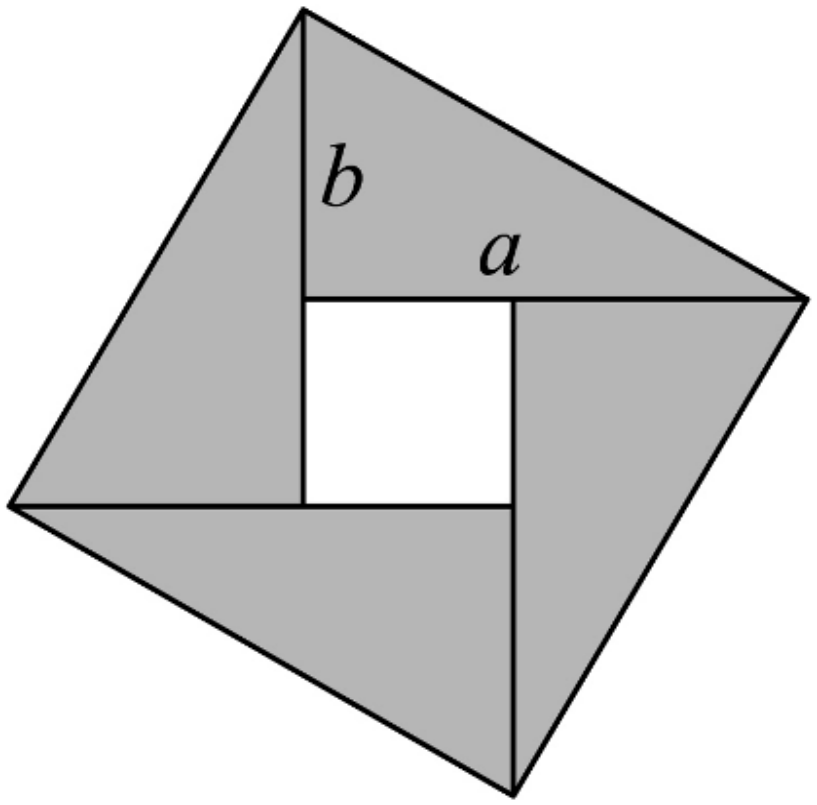
\includegraphics[width=0.20\textwidth]{figures/gao93_q16_zhaoshuang.png}
\end{center}

A. 如果 $a>b>0$，那么 $\sqrt a>\sqrt b$

B. 如果 $a>b>0$，那么 $a^2>b^2$

C. 对任意正实数 $a$ 和 $b$，有 $a^2+b^2\geqslant2ab$，当且仅当 $a=b$ 时等号成立

D. 对任意正实数 $a$ 和 $b$，有 $a^2+b^2\geqslant2ab$，当且仅当 $a=b$ 时等号成立% 原卷 C、D 两选项文字相同，照录

\ifanswer
\solbegin
\step{通过观察，可以发现这个图中的四个直角三角形是全等的，}
\step{设直角三角形的长直角边为 $a$，短直角边为 $b$，}
\step{如图，整个大正方形的面积大于等于这 $4$ 个直角三角形的面积和，}
\step{即 $a^2+b^2\geqslant4\times\left(\dfrac12ab\right)$，即 $a^2+b^2\geqslant2ab$，}
\step{当 $a=b$ 时，中间空白的正方形消失，即整个大正方形与 $4$ 个直角三角形重合；}
\step{其他选项通过该图无法证明. 故选 $C$.}
\solend
\fi

\end{enumerate}

\bigsec{三、解答题}

\begin{enumerate}
\setcounter{enumi}{16}

\item 已知 $x,y\in R$，比较 $x^2+y^2$ 与 $2(2x-y)-5$ 的大小.

\ansspace*[7]

\ifanswer
\solbegin
\step{因为 $x^2+y^2-2(2x-y)+5=(x-2)^2+(y+1)^2\geqslant0$，}
\step{所以 $x^2+y^2\geqslant2(2x-y)-5$.}
\solend
\fi

\item 设 $k\in\R$，求关于 $x$ 与 $y$ 的二元一次方程组 $\begin{cases}y=x+1\\ y=kx+3\end{cases}$ 的解集.

\ansspace*[9]

\ifanswer
\solbegin
\step{因为 $\begin{cases}y=x+1\\ y=kx+3\end{cases}$，两式相减，得到 $(k-1)x=-2$，}
\step{当 $k\neq1$ 时，$x=-\dfrac{2}{k-1}$，代入方程组中的第一式，得到 $y=\dfrac{k-3}{k-1}$，}
\step{此时，原方程组的解集为 $\left\{\left(-\dfrac{2}{k-1},\dfrac{k-3}{k-1}\right)\right\}$，}
\step{当 $k=1$ 时，方程 $(k-1)x=-2$ 无解，从而原方程组无解，其解集为空集.}
\step{综上，当 $k\neq1$ 时，解集为 $\left\{\left(-\dfrac{2}{k-1},\dfrac{k-3}{k-1}\right)\right\}$，}
\step{当 $k=1$ 时，解集为空集.}
\solend
\fi

\item 解下列不等式与方程组.

（1）解含绝对值的不等式：$\lvert x+1\rvert\geqslant3x$；

（2）求解不等式组 $\begin{cases}x^2-4x+3\geqslant0\\ \dfrac{x+3}{2x-1}\geqslant2\end{cases}$.

\ansspace*[10]

\ifanswer
\solbegin
\stepm{（1）}{当 $x\leqslant0$ 时，不等式显然成立，}
\step{当 $x>0$ 时，则 $(x+1)^2\geqslant9x^2$，得 $8x^2-2x-1\leqslant0$，}
\step{得 $(2x-1)(4x+1)\leqslant0$，解得 $-\dfrac14\leqslant x\leqslant\dfrac12$，由于 $x>0$，得 $0<x\leqslant\dfrac12$，}
\step{综上，不等式解集为 $\left\{x\left|x\leqslant\dfrac12\right.\right\}$.}
\stepm{（2）}{由 $x^2-4x+3\geqslant0$ 得 $(x-1)(x-3)\geqslant0$，所以 $x\leqslant1$ 或 $x\geqslant3$；}
\step{由 $\dfrac{x+3}{2x-1}\geqslant2$，得 $\dfrac{x+3}{2x-1}-2=\dfrac{-3x+5}{2x-1}\geqslant0$，即 $\dfrac{3x-5}{2x-1}\leqslant0$，}
\step{所以 $\begin{cases}(3x-5)(2x-1)\leqslant0\\ 2x-1\neq0\end{cases}$，解得 $\dfrac12<x\leqslant\dfrac53$，}
\step{所以不等式组的解集是 $\left\{x\left|\dfrac12<x\leqslant1\right.\right\}$.}
\solend
\fi

\item 已知关于 $x$ 的不等式 $2kx^2+kx-1<0$.

（1）若不等式的解集为 $\left(-\dfrac32,1\right)$，求实数 $k$ 的值；

（2）若不等式的解集为 $R$，求实数 $k$ 的取值范围.

\ansspace*[11]

\ifanswer
\solbegin
\stepm{（1）}{关于 $x$ 的不等式 $2kx^2+kx-1<0$ 的解集为 $\left(-\dfrac32,1\right)$，}
\step{所以 $-\dfrac32$ 和 $1$ 是方程 $2kx^2+kx-1=0$ 的两个实数根，}
\step{代入 $x=1$ 得 $2k+k-1=0$，解得 $k=\dfrac13$；}
\stepm{（2）}{若不等式 $2kx^2+kx-1<0$ 的解集为 $R$，}
\step{则 $k=0$ 时，不等式为 $-1<0$，满足题意；}
\step{$k\neq0$ 时，应满足 $\begin{cases}k<0\\ \Delta=k^2+8k<0\end{cases}$，解得 $-8<k<0$；}
\step{综上，实数 $k$ 的取值范围是 $-8<k\leqslant0$.}
\solend
\fi

\item 国家为了加强对烟酒生产的宏观管理，实行征收附加税政策，现知某种酒每瓶 $70$ 元，不征收附加税的时候，每年大约产销 $100$ 万瓶，若政府征收附加税，每销售 $100$ 元要征税 $R$ 元（叫做税率 $R\%$），则每年的销售将减少 $10R$ 万瓶.

（1）求出每年商店经营烟酒被征收的附加税税金 $S$（单位：万元）；

（2）若附加税税金 $S$ 不少于 $112$ 万元，且不大于 $168$ 万元，求 $R$ 的取值范围.

\ansspace*[12]

\ifanswer
\solbegin
\stepm{（1）}{由题意得 $S=70\times(100-10R)\times R\%(0\leqslant R\leqslant10)$（单位：万元）.}
\stepm{（2）}{由题意 $\begin{cases}70\times(100-10R)\times R\%\geqslant112\\ 70\times(100-10R)\times R\%\leqslant168\end{cases}$，解得 $2\leqslant R\leqslant4$ 或 $6\leqslant R\leqslant8$，}
\step{所以 $R$ 的取值范围是 $[2,4]\cup[6,8]$.}
\solend
\fi

\end{enumerate}

\end{document}
"
% 紧凑版：xelatex "\def\iscompact{1}% 高一93_建平世纪_10月月考.tex
%   —— 高一上数学“2026-2027 年建平世纪高一上 10 月月考”（讲评版）
% 试卷版：xelatex 高一93_建平世纪_10月月考.tex
% 答案版：xelatex "\def\isanswer{1}\input{高一93_建平世纪_10月月考.tex}"
% 紧凑版：xelatex "\def\iscompact{1}\input{高一93_建平世纪_10月月考.tex}"
%
% 原始材料：微信公众号“魔都数学加油站”文章，连载“27学年高一93”；
% 原文标题“27学年高一93——2026-2027年上海市建平世纪高一上10月月考”；
% 原文链接：https://mp.weixin.qq.com/s/uqySZX3I8Q-QZ2J8MqmWiA。
% 正文为 7 张 PNG 页（`原图/高一93_建平世纪_10月月考/01..07.png`），均 4762×6735，按页序读取。
%
% 篇幅与题号：原卷自第 3 题起编号（第 1、2 题不在原文内）。填空题 3—12（10 题）、
% 选择题 13—16（4 题）、解答题 17—21（5 题），共 19 题。
%
% 讲评版：第 3、4 题只印【答案】（“$\{x\mid-1<x<1\}$”“$x$ 和 $y$ 不都是有理数”），本稿只给 \ans{}；
% 其余 17 题印【解析】，其中选择题答案在解析末句“故选 $D$／$D$／$C$／$C$”。
% 第 16 题题干右侧有一幅赵爽弦图（裁自第 4 页原图、去粉色水印后转灰度）。
%
% 副标题：原卷未印副标题。本稿按内容标作“集合与常用逻辑用语、不等式”。
%
% 原卷笔误/存疑（均照录未改，正文对应处另有 % 注）：
%   ① 第 3 题答案印作 $\{x\mid-1<x<1\}$（两端开），而 $\lvert x\rvert\leqslant1$ 的解集应为
%      $[-1,1]$（两端闭）；原卷照录，未改；
%   ② 第 16 题 C、D 两个选项**文字完全相同**（皆为“对任意正实数 $a$ 和 $b$，有
%      $a^2+b^2\geqslant2ab$，当且仅当 $a=b$ 时等号成立”），原卷重复排印；答案取 $C$，
%      本稿两个选项照录。
%
% 与原卷的排版差异：
%   ① 原卷每题下直接印【答案】/【解析】，本稿按全稿惯例将答案与解析置于答案版；
%   ② 原卷未印副标题，本稿补出；填空横线统一排 \blankline[4.4em]；
%   ③ 原卷数集记号排斜体 $R$，本稿按全稿惯例改用 $\R$；
%   ④ 第 17—21 题的子问用行内“（1）（2）（3）”段，解析中的子问标号用 \stepm；
%   ⑤ 解答题按惯例加 \ansspace；选择题括号排 \mbox{（\quad）}；
%   ⑥ 第 16 题的弦图原卷排在题干右侧、文字绕排，本稿改排为选项后的居中图。
%
% 行数核对：逐题数 \step/\stepm 条数，合计 71 条（Q3：0；Q4：0；Q5：2；Q6：3；Q7：2；
% Q8：2；Q9：4；Q10：1；Q11：3；Q12：9；Q13：5；Q14：3；Q15：5；Q16：6；Q17：2；
% Q18：6；Q19：8；Q20：7；Q21：3）。第 3、4 题只印答案，不计入 \step 账。
% 原卷解析的换行按语意合并，未逐行强拆。
%
\documentclass[a4paper,11pt]{article}
\usepackage{common}

\begin{document}

\examtitlest[7]{2026--2027 年建平世纪高一上 10 月月考}{集合与常用逻辑用语、不等式}

\bigsec{一、填空题}

\begin{enumerate}
\setcounter{enumi}{2}

\item 不等式 $\lvert x\rvert\leqslant1$ 的解集是\blankline[4.4em].

\ifanswer
\ans{$\{x\mid-1<x<1\}$}% 原卷答案两端开；|x|≤1 应为 [-1,1]，照录
\fi

\item “$x$ 和 $y$ 都是有理数”的否定形式是\blankline[4.4em].

\ifanswer
\ans{$x$ 和 $y$ 不都是有理数}
\fi

\item 已知等式 $2x^2+3x+5=2ax^2+a(3x+1)+c$ 恒成立，则 $a+c=\blankline[4.4em]$.

\ifanswer
\solbegin
\step{因为 $2x^2+3x+5=2ax^2+a(3x+1)+c$ 恒成立，}
\step{即 $2x^2+3x+5=2ax^2+3ax+(a+c)$ 恒成立，所以 $\begin{cases}2=2a\\ 3=3a\\ 5=a+c\end{cases}$，所以 $a+c=5$.}
\solend
\fi

\item 已知方程 $x^2+6x+m=0(m\in\R)$ 的两个根 $x_1$、$x_2$ 满足 $\lvert x_1-x_2\rvert=4$，则 $m$ 的值是\blankline[4.4em].

\ifanswer
\solbegin
\step{方程 $x^2+6x+m=0(m\in\R)$ 的两根为 $x_1$、$x_2$，所以 $x_1+x_2=-6$，$x_1x_2=m$，}
\step{又 $\lvert x_1-x_2\rvert=4$，则 $(x_1-x_2)^2=(x_1+x_2)^2-4x_1x_2=16$，}
\step{即 $(-6)^2-4m=16$，解得 $m=5$，检验得 $\Delta=6^2-4\times1\times5=16>0$，符合题意，所以 $m=5$.}
\solend
\fi

\item 已知 $\alpha:2m-6<x<m+5$，$\beta:-3<x<5$，若 $\alpha$ 是 $\beta$ 的必要条件，则实数 $m$ 的取值范围是\blankline[4.4em].

\ifanswer
\solbegin
\step{因为 $\alpha$ 是 $\beta$ 的必要条件，所以 $\begin{cases}2m-6\leqslant-3\\ m+5\geqslant5\\ 2m-6<m+5\end{cases}\Rightarrow0\leqslant m\leqslant\dfrac32$，}
\step{所以实数 $m$ 的取值范围是 $\left[0,\dfrac32\right]$.}
\solend
\fi

\item 已知 $-2\leqslant a\leqslant3$，$2\leqslant b\leqslant\dfrac72$，则 $a-2b$ 的取值范围为\blankline[4.4em].

\ifanswer
\solbegin
\step{因为 $-2\leqslant a\leqslant3$，$2\leqslant b\leqslant\dfrac72$，所以 $-7\leqslant-2b\leqslant-4$，所以 $-9\leqslant a-2b\leqslant-1$，}
\step{故 $a-2b$ 的取值范围为 $[-9,-1]$.}
\solend
\fi

\item 已知 $\lvert x+3\rvert+\lvert5-x\rvert>10$，则实数 $x$ 的取值范围为\blankline[4.4em].

\ifanswer
\solbegin
\step{当 $x<-3$ 时，则 $-x-3+5-x>10$，解得 $x<-4$，}
\step{当 $-3\leqslant x\leqslant5$ 时，则 $x+3+5-x=8<10$，原不等式不成立，}
\step{当 $x>5$ 时，则 $x+3+x-5>10$，解得 $x>6$，}
\step{综上所述，实数 $x$ 的取值范围为 $(-\infty,-4)\cup(6,+\infty)$.}
\solend
\fi

\item 已知集合 $A=\{(x,y)\mid y=x+1\}$，$B=\{(x,y)\mid y=-x+3\}$，则 $A\cap B=\blankline[4.4em]$.

\ifanswer
\solbegin
\step{联立 $\begin{cases}y=x+1\\ y=-x+3\end{cases}$，解得 $x=1$，$y=2$，故 $A\cap B=\{(1,2)\}$.}
\solend
\fi

\item 若关于 $x$ 的不等式组 $\begin{cases}\dfrac{x-1}{x-3}<0\\ x>a\end{cases}$ 的解集为空集，则实数 $a$ 的取值范围为\blankline[4.4em].

\ifanswer
\solbegin
\step{$\dfrac{x-1}{x-3}<0$ 等价于 $(x-1)(x-3)<0$，得 $1<x<3$，}
\step{因为 $\begin{cases}\dfrac{x-1}{x-3}<0\\ x>a\end{cases}$ 的解集为空集，}
\step{所以 $a\geqslant3$，故实数 $a$ 的取值范围为 $[3,+\infty)$.}
\solend
\fi

\item 已知由自然数组成的 $n-1$ 个元素的集合 $A=\{1,2,3,4,\cdots,n-1\}(n>1)$，非空集合 $B\subseteq A$，且对任意的 $a\in B$，都有 $n-a\in B$. 当 $n=9$ 时，则所有满足条件的集合 $B$ 的元素的和为\blankline[4.4em].

\ifanswer
\solbegin
\step{当 $n=9$ 时，$A=\{1,2,3,4,5,6,7,8\}$，}
\step{当 $B$ 中有两个元素时，集合 $B$ 可以为 $\{1,8\},\{2,7\},\{3,6\},\{4,5\}$，}
\step{元素总和为 $4\times9=36$；}
\step{当 $B$ 中有四个元素时，集合 $B$ 可以为 $\{1,8\},\{2,7\},\{3,6\},\{4,5\}$ 中任取两个的并集，}
\step{集合 $B$ 共有 $6$ 种情况，元素总和为 $6\times2\times9=108$；}
\step{当 $B$ 中有六个元素时，集合 $B$ 可以为 $\{1,8\},\{2,7\},\{3,6\},\{4,5\}$ 中任取三个的并集，}
\step{集合 $B$ 共有 $4$ 种情况，元素总和为 $4\times3\times9=12\times9=108$；}
\step{当 $B$ 中有八个元素时，$B=\{1,2,3,4,5,6,7,8\}$，元素之和为 $4\times9=36$，}
\step{所以所有满足条件的集合 $B$ 的元素总和为 $36+108+108+36=288$.}
\solend
\fi

\end{enumerate}

\bigsec{二、选择题}

\begin{enumerate}
\setcounter{enumi}{12}

\item 下列说法正确的是\mbox{（\quad）}

\keepwithprev
A. 若 $a>b$，则 $\dfrac1a<\dfrac1b$\qquad B. 若 $a>b,c>d$，则 $ac>bd$

C. 若 $a>b$，则 $ac^2>bc^2$\qquad D. 若 $ac^2>bc^2$，则 $a>b$

\ifanswer
\solbegin
\step{A：令 $a=2,b=-1$，此时 $\dfrac12>-1$，故 A 错误；}
\step{B：令 $a=2,b=-1,c=0,d=-2$，此时 $ac=0<bd=2$，故 B 错误；}
\step{C：由 $a>b$，当 $c=0$ 时，$ac^2=bc^2$，故 C 错误；}
\step{D：由 $ac^2>bc^2$，则 $c^2>0$，所以 $a>b$，故 D 正确.}
\step{故选 $D$.}
\solend
\fi

\item 不等式 $\dfrac{x-3}{x-1}\leqslant2$ 的解集是\mbox{（\quad）}

\keepwithprev
A. $(-\infty,1]$\qquad B. $[1,+\infty)$

C. $(-\infty,-1]\cup[1,+\infty)$\qquad D. $(-\infty,-1]\cup(1,+\infty)$

\ifanswer
\solbegin
\step{不等式 $\dfrac{x-3}{x-1}\leqslant2$ 可化为 $\dfrac{x-3}{x-1}-2\leqslant0$，即 $\dfrac{x-3-2(x-1)}{x-1}\leqslant0$，}
\step{化简得 $\dfrac{x+1}{x-1}\geqslant0$，等价于 $\begin{cases}(x+1)(x-1)\geqslant0\\ x\neq1\end{cases}$，解得 $x\leqslant-1$ 或 $x>1$，}
\step{所以不等式的解集为 $(-\infty,-1]\cup(1,+\infty)$. 故选 $D$.}
\solend
\fi

\item 已知集合 $M$ 和集合 $N$，那么 $M\cap N=N$ 的充要条件是\mbox{（\quad）}

\keepwithprev
A. $M\subseteq N$\qquad B. $N\subset M$\qquad C. $M\supseteq N$\qquad D. $M=N$

\ifanswer
\solbegin
\step{若 $M\subseteq N$，即集合 $M$ 是集合 $N$ 的子集，则 $M\cap N=M$，故 $A$ 错误；}
\step{若 $M=N$，则不能得到 $N\subset M$，故 $B$ 错误；}
\step{若 $M\cap N=N$，则 $M\supseteq N$，故 $C$ 正确；}
\step{当 $N$ 是 $M$ 真子集时，不能得到 $M=N$，故 $D$ 错误.}
\step{故选 $C$.}
\solend
\fi

\item 三国时期赵爽在《勾股方圆图注》中对勾股定理的证明可用现代数学表述为如图所示，我们教材中利用该图作为“（\quad）”的几何解释.

\begin{center}
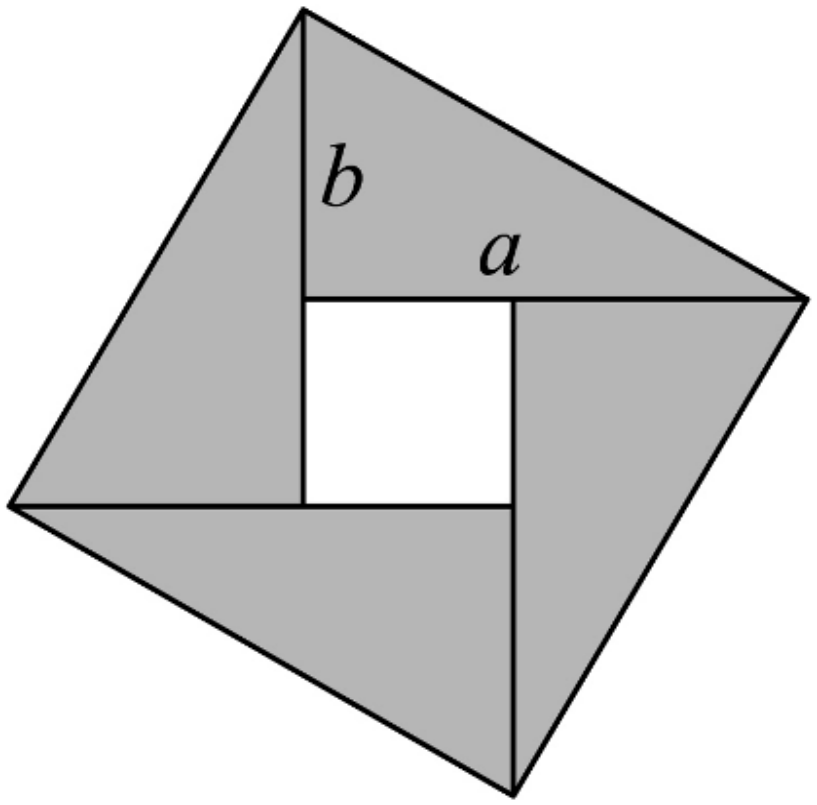
\includegraphics[width=0.20\textwidth]{figures/gao93_q16_zhaoshuang.png}
\end{center}

A. 如果 $a>b>0$，那么 $\sqrt a>\sqrt b$

B. 如果 $a>b>0$，那么 $a^2>b^2$

C. 对任意正实数 $a$ 和 $b$，有 $a^2+b^2\geqslant2ab$，当且仅当 $a=b$ 时等号成立

D. 对任意正实数 $a$ 和 $b$，有 $a^2+b^2\geqslant2ab$，当且仅当 $a=b$ 时等号成立% 原卷 C、D 两选项文字相同，照录

\ifanswer
\solbegin
\step{通过观察，可以发现这个图中的四个直角三角形是全等的，}
\step{设直角三角形的长直角边为 $a$，短直角边为 $b$，}
\step{如图，整个大正方形的面积大于等于这 $4$ 个直角三角形的面积和，}
\step{即 $a^2+b^2\geqslant4\times\left(\dfrac12ab\right)$，即 $a^2+b^2\geqslant2ab$，}
\step{当 $a=b$ 时，中间空白的正方形消失，即整个大正方形与 $4$ 个直角三角形重合；}
\step{其他选项通过该图无法证明. 故选 $C$.}
\solend
\fi

\end{enumerate}

\bigsec{三、解答题}

\begin{enumerate}
\setcounter{enumi}{16}

\item 已知 $x,y\in R$，比较 $x^2+y^2$ 与 $2(2x-y)-5$ 的大小.

\ansspace*[7]

\ifanswer
\solbegin
\step{因为 $x^2+y^2-2(2x-y)+5=(x-2)^2+(y+1)^2\geqslant0$，}
\step{所以 $x^2+y^2\geqslant2(2x-y)-5$.}
\solend
\fi

\item 设 $k\in\R$，求关于 $x$ 与 $y$ 的二元一次方程组 $\begin{cases}y=x+1\\ y=kx+3\end{cases}$ 的解集.

\ansspace*[9]

\ifanswer
\solbegin
\step{因为 $\begin{cases}y=x+1\\ y=kx+3\end{cases}$，两式相减，得到 $(k-1)x=-2$，}
\step{当 $k\neq1$ 时，$x=-\dfrac{2}{k-1}$，代入方程组中的第一式，得到 $y=\dfrac{k-3}{k-1}$，}
\step{此时，原方程组的解集为 $\left\{\left(-\dfrac{2}{k-1},\dfrac{k-3}{k-1}\right)\right\}$，}
\step{当 $k=1$ 时，方程 $(k-1)x=-2$ 无解，从而原方程组无解，其解集为空集.}
\step{综上，当 $k\neq1$ 时，解集为 $\left\{\left(-\dfrac{2}{k-1},\dfrac{k-3}{k-1}\right)\right\}$，}
\step{当 $k=1$ 时，解集为空集.}
\solend
\fi

\item 解下列不等式与方程组.

（1）解含绝对值的不等式：$\lvert x+1\rvert\geqslant3x$；

（2）求解不等式组 $\begin{cases}x^2-4x+3\geqslant0\\ \dfrac{x+3}{2x-1}\geqslant2\end{cases}$.

\ansspace*[10]

\ifanswer
\solbegin
\stepm{（1）}{当 $x\leqslant0$ 时，不等式显然成立，}
\step{当 $x>0$ 时，则 $(x+1)^2\geqslant9x^2$，得 $8x^2-2x-1\leqslant0$，}
\step{得 $(2x-1)(4x+1)\leqslant0$，解得 $-\dfrac14\leqslant x\leqslant\dfrac12$，由于 $x>0$，得 $0<x\leqslant\dfrac12$，}
\step{综上，不等式解集为 $\left\{x\left|x\leqslant\dfrac12\right.\right\}$.}
\stepm{（2）}{由 $x^2-4x+3\geqslant0$ 得 $(x-1)(x-3)\geqslant0$，所以 $x\leqslant1$ 或 $x\geqslant3$；}
\step{由 $\dfrac{x+3}{2x-1}\geqslant2$，得 $\dfrac{x+3}{2x-1}-2=\dfrac{-3x+5}{2x-1}\geqslant0$，即 $\dfrac{3x-5}{2x-1}\leqslant0$，}
\step{所以 $\begin{cases}(3x-5)(2x-1)\leqslant0\\ 2x-1\neq0\end{cases}$，解得 $\dfrac12<x\leqslant\dfrac53$，}
\step{所以不等式组的解集是 $\left\{x\left|\dfrac12<x\leqslant1\right.\right\}$.}
\solend
\fi

\item 已知关于 $x$ 的不等式 $2kx^2+kx-1<0$.

（1）若不等式的解集为 $\left(-\dfrac32,1\right)$，求实数 $k$ 的值；

（2）若不等式的解集为 $R$，求实数 $k$ 的取值范围.

\ansspace*[11]

\ifanswer
\solbegin
\stepm{（1）}{关于 $x$ 的不等式 $2kx^2+kx-1<0$ 的解集为 $\left(-\dfrac32,1\right)$，}
\step{所以 $-\dfrac32$ 和 $1$ 是方程 $2kx^2+kx-1=0$ 的两个实数根，}
\step{代入 $x=1$ 得 $2k+k-1=0$，解得 $k=\dfrac13$；}
\stepm{（2）}{若不等式 $2kx^2+kx-1<0$ 的解集为 $R$，}
\step{则 $k=0$ 时，不等式为 $-1<0$，满足题意；}
\step{$k\neq0$ 时，应满足 $\begin{cases}k<0\\ \Delta=k^2+8k<0\end{cases}$，解得 $-8<k<0$；}
\step{综上，实数 $k$ 的取值范围是 $-8<k\leqslant0$.}
\solend
\fi

\item 国家为了加强对烟酒生产的宏观管理，实行征收附加税政策，现知某种酒每瓶 $70$ 元，不征收附加税的时候，每年大约产销 $100$ 万瓶，若政府征收附加税，每销售 $100$ 元要征税 $R$ 元（叫做税率 $R\%$），则每年的销售将减少 $10R$ 万瓶.

（1）求出每年商店经营烟酒被征收的附加税税金 $S$（单位：万元）；

（2）若附加税税金 $S$ 不少于 $112$ 万元，且不大于 $168$ 万元，求 $R$ 的取值范围.

\ansspace*[12]

\ifanswer
\solbegin
\stepm{（1）}{由题意得 $S=70\times(100-10R)\times R\%(0\leqslant R\leqslant10)$（单位：万元）.}
\stepm{（2）}{由题意 $\begin{cases}70\times(100-10R)\times R\%\geqslant112\\ 70\times(100-10R)\times R\%\leqslant168\end{cases}$，解得 $2\leqslant R\leqslant4$ 或 $6\leqslant R\leqslant8$，}
\step{所以 $R$ 的取值范围是 $[2,4]\cup[6,8]$.}
\solend
\fi

\end{enumerate}

\end{document}
"
%
% 原始材料：微信公众号“魔都数学加油站”文章，连载“27学年高一93”；
% 原文标题“27学年高一93——2026-2027年上海市建平世纪高一上10月月考”；
% 原文链接：https://mp.weixin.qq.com/s/uqySZX3I8Q-QZ2J8MqmWiA。
% 正文为 7 张 PNG 页（`原图/高一93_建平世纪_10月月考/01..07.png`），均 4762×6735，按页序读取。
%
% 篇幅与题号：原卷自第 3 题起编号（第 1、2 题不在原文内）。填空题 3—12（10 题）、
% 选择题 13—16（4 题）、解答题 17—21（5 题），共 19 题。
%
% 讲评版：第 3、4 题只印【答案】（“$\{x\mid-1<x<1\}$”“$x$ 和 $y$ 不都是有理数”），本稿只给 \ans{}；
% 其余 17 题印【解析】，其中选择题答案在解析末句“故选 $D$／$D$／$C$／$C$”。
% 第 16 题题干右侧有一幅赵爽弦图（裁自第 4 页原图、去粉色水印后转灰度）。
%
% 副标题：原卷未印副标题。本稿按内容标作“集合与常用逻辑用语、不等式”。
%
% 原卷笔误/存疑（均照录未改，正文对应处另有 % 注）：
%   ① 第 3 题答案印作 $\{x\mid-1<x<1\}$（两端开），而 $\lvert x\rvert\leqslant1$ 的解集应为
%      $[-1,1]$（两端闭）；原卷照录，未改；
%   ② 第 16 题 C、D 两个选项**文字完全相同**（皆为“对任意正实数 $a$ 和 $b$，有
%      $a^2+b^2\geqslant2ab$，当且仅当 $a=b$ 时等号成立”），原卷重复排印；答案取 $C$，
%      本稿两个选项照录。
%
% 与原卷的排版差异：
%   ① 原卷每题下直接印【答案】/【解析】，本稿按全稿惯例将答案与解析置于答案版；
%   ② 原卷未印副标题，本稿补出；填空横线统一排 \blankline[4.4em]；
%   ③ 原卷数集记号排斜体 $R$，本稿按全稿惯例改用 $\R$；
%   ④ 第 17—21 题的子问用行内“（1）（2）（3）”段，解析中的子问标号用 \stepm；
%   ⑤ 解答题按惯例加 \ansspace；选择题括号排 \mbox{（\quad）}；
%   ⑥ 第 16 题的弦图原卷排在题干右侧、文字绕排，本稿改排为选项后的居中图。
%
% 行数核对：逐题数 \step/\stepm 条数，合计 71 条（Q3：0；Q4：0；Q5：2；Q6：3；Q7：2；
% Q8：2；Q9：4；Q10：1；Q11：3；Q12：9；Q13：5；Q14：3；Q15：5；Q16：6；Q17：2；
% Q18：6；Q19：8；Q20：7；Q21：3）。第 3、4 题只印答案，不计入 \step 账。
% 原卷解析的换行按语意合并，未逐行强拆。
%
\documentclass[a4paper,11pt]{article}
\usepackage{common}

\begin{document}

\examtitlest[7]{2026--2027 年建平世纪高一上 10 月月考}{集合与常用逻辑用语、不等式}

\bigsec{一、填空题}

\begin{enumerate}
\setcounter{enumi}{2}

\item 不等式 $\lvert x\rvert\leqslant1$ 的解集是\blankline[4.4em].

\ifanswer
\ans{$\{x\mid-1<x<1\}$}% 原卷答案两端开；|x|≤1 应为 [-1,1]，照录
\fi

\item “$x$ 和 $y$ 都是有理数”的否定形式是\blankline[4.4em].

\ifanswer
\ans{$x$ 和 $y$ 不都是有理数}
\fi

\item 已知等式 $2x^2+3x+5=2ax^2+a(3x+1)+c$ 恒成立，则 $a+c=\blankline[4.4em]$.

\ifanswer
\solbegin
\step{因为 $2x^2+3x+5=2ax^2+a(3x+1)+c$ 恒成立，}
\step{即 $2x^2+3x+5=2ax^2+3ax+(a+c)$ 恒成立，所以 $\begin{cases}2=2a\\ 3=3a\\ 5=a+c\end{cases}$，所以 $a+c=5$.}
\solend
\fi

\item 已知方程 $x^2+6x+m=0(m\in\R)$ 的两个根 $x_1$、$x_2$ 满足 $\lvert x_1-x_2\rvert=4$，则 $m$ 的值是\blankline[4.4em].

\ifanswer
\solbegin
\step{方程 $x^2+6x+m=0(m\in\R)$ 的两根为 $x_1$、$x_2$，所以 $x_1+x_2=-6$，$x_1x_2=m$，}
\step{又 $\lvert x_1-x_2\rvert=4$，则 $(x_1-x_2)^2=(x_1+x_2)^2-4x_1x_2=16$，}
\step{即 $(-6)^2-4m=16$，解得 $m=5$，检验得 $\Delta=6^2-4\times1\times5=16>0$，符合题意，所以 $m=5$.}
\solend
\fi

\item 已知 $\alpha:2m-6<x<m+5$，$\beta:-3<x<5$，若 $\alpha$ 是 $\beta$ 的必要条件，则实数 $m$ 的取值范围是\blankline[4.4em].

\ifanswer
\solbegin
\step{因为 $\alpha$ 是 $\beta$ 的必要条件，所以 $\begin{cases}2m-6\leqslant-3\\ m+5\geqslant5\\ 2m-6<m+5\end{cases}\Rightarrow0\leqslant m\leqslant\dfrac32$，}
\step{所以实数 $m$ 的取值范围是 $\left[0,\dfrac32\right]$.}
\solend
\fi

\item 已知 $-2\leqslant a\leqslant3$，$2\leqslant b\leqslant\dfrac72$，则 $a-2b$ 的取值范围为\blankline[4.4em].

\ifanswer
\solbegin
\step{因为 $-2\leqslant a\leqslant3$，$2\leqslant b\leqslant\dfrac72$，所以 $-7\leqslant-2b\leqslant-4$，所以 $-9\leqslant a-2b\leqslant-1$，}
\step{故 $a-2b$ 的取值范围为 $[-9,-1]$.}
\solend
\fi

\item 已知 $\lvert x+3\rvert+\lvert5-x\rvert>10$，则实数 $x$ 的取值范围为\blankline[4.4em].

\ifanswer
\solbegin
\step{当 $x<-3$ 时，则 $-x-3+5-x>10$，解得 $x<-4$，}
\step{当 $-3\leqslant x\leqslant5$ 时，则 $x+3+5-x=8<10$，原不等式不成立，}
\step{当 $x>5$ 时，则 $x+3+x-5>10$，解得 $x>6$，}
\step{综上所述，实数 $x$ 的取值范围为 $(-\infty,-4)\cup(6,+\infty)$.}
\solend
\fi

\item 已知集合 $A=\{(x,y)\mid y=x+1\}$，$B=\{(x,y)\mid y=-x+3\}$，则 $A\cap B=\blankline[4.4em]$.

\ifanswer
\solbegin
\step{联立 $\begin{cases}y=x+1\\ y=-x+3\end{cases}$，解得 $x=1$，$y=2$，故 $A\cap B=\{(1,2)\}$.}
\solend
\fi

\item 若关于 $x$ 的不等式组 $\begin{cases}\dfrac{x-1}{x-3}<0\\ x>a\end{cases}$ 的解集为空集，则实数 $a$ 的取值范围为\blankline[4.4em].

\ifanswer
\solbegin
\step{$\dfrac{x-1}{x-3}<0$ 等价于 $(x-1)(x-3)<0$，得 $1<x<3$，}
\step{因为 $\begin{cases}\dfrac{x-1}{x-3}<0\\ x>a\end{cases}$ 的解集为空集，}
\step{所以 $a\geqslant3$，故实数 $a$ 的取值范围为 $[3,+\infty)$.}
\solend
\fi

\item 已知由自然数组成的 $n-1$ 个元素的集合 $A=\{1,2,3,4,\cdots,n-1\}(n>1)$，非空集合 $B\subseteq A$，且对任意的 $a\in B$，都有 $n-a\in B$. 当 $n=9$ 时，则所有满足条件的集合 $B$ 的元素的和为\blankline[4.4em].

\ifanswer
\solbegin
\step{当 $n=9$ 时，$A=\{1,2,3,4,5,6,7,8\}$，}
\step{当 $B$ 中有两个元素时，集合 $B$ 可以为 $\{1,8\},\{2,7\},\{3,6\},\{4,5\}$，}
\step{元素总和为 $4\times9=36$；}
\step{当 $B$ 中有四个元素时，集合 $B$ 可以为 $\{1,8\},\{2,7\},\{3,6\},\{4,5\}$ 中任取两个的并集，}
\step{集合 $B$ 共有 $6$ 种情况，元素总和为 $6\times2\times9=108$；}
\step{当 $B$ 中有六个元素时，集合 $B$ 可以为 $\{1,8\},\{2,7\},\{3,6\},\{4,5\}$ 中任取三个的并集，}
\step{集合 $B$ 共有 $4$ 种情况，元素总和为 $4\times3\times9=12\times9=108$；}
\step{当 $B$ 中有八个元素时，$B=\{1,2,3,4,5,6,7,8\}$，元素之和为 $4\times9=36$，}
\step{所以所有满足条件的集合 $B$ 的元素总和为 $36+108+108+36=288$.}
\solend
\fi

\end{enumerate}

\bigsec{二、选择题}

\begin{enumerate}
\setcounter{enumi}{12}

\item 下列说法正确的是\mbox{（\quad）}

\keepwithprev
A. 若 $a>b$，则 $\dfrac1a<\dfrac1b$\qquad B. 若 $a>b,c>d$，则 $ac>bd$

C. 若 $a>b$，则 $ac^2>bc^2$\qquad D. 若 $ac^2>bc^2$，则 $a>b$

\ifanswer
\solbegin
\step{A：令 $a=2,b=-1$，此时 $\dfrac12>-1$，故 A 错误；}
\step{B：令 $a=2,b=-1,c=0,d=-2$，此时 $ac=0<bd=2$，故 B 错误；}
\step{C：由 $a>b$，当 $c=0$ 时，$ac^2=bc^2$，故 C 错误；}
\step{D：由 $ac^2>bc^2$，则 $c^2>0$，所以 $a>b$，故 D 正确.}
\step{故选 $D$.}
\solend
\fi

\item 不等式 $\dfrac{x-3}{x-1}\leqslant2$ 的解集是\mbox{（\quad）}

\keepwithprev
A. $(-\infty,1]$\qquad B. $[1,+\infty)$

C. $(-\infty,-1]\cup[1,+\infty)$\qquad D. $(-\infty,-1]\cup(1,+\infty)$

\ifanswer
\solbegin
\step{不等式 $\dfrac{x-3}{x-1}\leqslant2$ 可化为 $\dfrac{x-3}{x-1}-2\leqslant0$，即 $\dfrac{x-3-2(x-1)}{x-1}\leqslant0$，}
\step{化简得 $\dfrac{x+1}{x-1}\geqslant0$，等价于 $\begin{cases}(x+1)(x-1)\geqslant0\\ x\neq1\end{cases}$，解得 $x\leqslant-1$ 或 $x>1$，}
\step{所以不等式的解集为 $(-\infty,-1]\cup(1,+\infty)$. 故选 $D$.}
\solend
\fi

\item 已知集合 $M$ 和集合 $N$，那么 $M\cap N=N$ 的充要条件是\mbox{（\quad）}

\keepwithprev
A. $M\subseteq N$\qquad B. $N\subset M$\qquad C. $M\supseteq N$\qquad D. $M=N$

\ifanswer
\solbegin
\step{若 $M\subseteq N$，即集合 $M$ 是集合 $N$ 的子集，则 $M\cap N=M$，故 $A$ 错误；}
\step{若 $M=N$，则不能得到 $N\subset M$，故 $B$ 错误；}
\step{若 $M\cap N=N$，则 $M\supseteq N$，故 $C$ 正确；}
\step{当 $N$ 是 $M$ 真子集时，不能得到 $M=N$，故 $D$ 错误.}
\step{故选 $C$.}
\solend
\fi

\item 三国时期赵爽在《勾股方圆图注》中对勾股定理的证明可用现代数学表述为如图所示，我们教材中利用该图作为“（\quad）”的几何解释.

\begin{center}
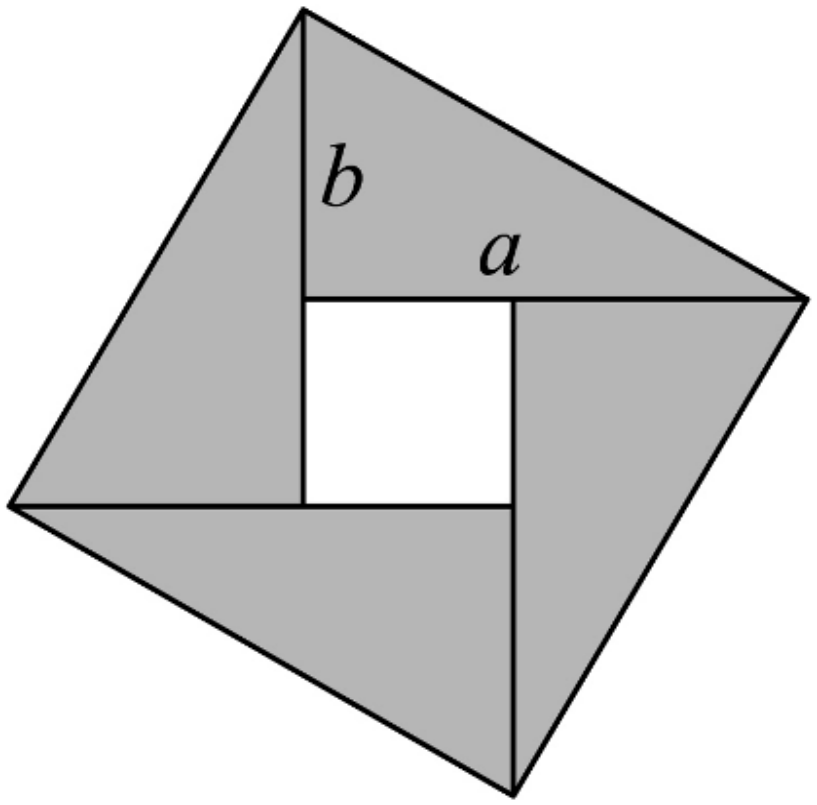
\includegraphics[width=0.20\textwidth]{figures/gao93_q16_zhaoshuang.png}
\end{center}

A. 如果 $a>b>0$，那么 $\sqrt a>\sqrt b$

B. 如果 $a>b>0$，那么 $a^2>b^2$

C. 对任意正实数 $a$ 和 $b$，有 $a^2+b^2\geqslant2ab$，当且仅当 $a=b$ 时等号成立

D. 对任意正实数 $a$ 和 $b$，有 $a^2+b^2\geqslant2ab$，当且仅当 $a=b$ 时等号成立% 原卷 C、D 两选项文字相同，照录

\ifanswer
\solbegin
\step{通过观察，可以发现这个图中的四个直角三角形是全等的，}
\step{设直角三角形的长直角边为 $a$，短直角边为 $b$，}
\step{如图，整个大正方形的面积大于等于这 $4$ 个直角三角形的面积和，}
\step{即 $a^2+b^2\geqslant4\times\left(\dfrac12ab\right)$，即 $a^2+b^2\geqslant2ab$，}
\step{当 $a=b$ 时，中间空白的正方形消失，即整个大正方形与 $4$ 个直角三角形重合；}
\step{其他选项通过该图无法证明. 故选 $C$.}
\solend
\fi

\end{enumerate}

\bigsec{三、解答题}

\begin{enumerate}
\setcounter{enumi}{16}

\item 已知 $x,y\in R$，比较 $x^2+y^2$ 与 $2(2x-y)-5$ 的大小.

\ansspace*[7]

\ifanswer
\solbegin
\step{因为 $x^2+y^2-2(2x-y)+5=(x-2)^2+(y+1)^2\geqslant0$，}
\step{所以 $x^2+y^2\geqslant2(2x-y)-5$.}
\solend
\fi

\item 设 $k\in\R$，求关于 $x$ 与 $y$ 的二元一次方程组 $\begin{cases}y=x+1\\ y=kx+3\end{cases}$ 的解集.

\ansspace*[9]

\ifanswer
\solbegin
\step{因为 $\begin{cases}y=x+1\\ y=kx+3\end{cases}$，两式相减，得到 $(k-1)x=-2$，}
\step{当 $k\neq1$ 时，$x=-\dfrac{2}{k-1}$，代入方程组中的第一式，得到 $y=\dfrac{k-3}{k-1}$，}
\step{此时，原方程组的解集为 $\left\{\left(-\dfrac{2}{k-1},\dfrac{k-3}{k-1}\right)\right\}$，}
\step{当 $k=1$ 时，方程 $(k-1)x=-2$ 无解，从而原方程组无解，其解集为空集.}
\step{综上，当 $k\neq1$ 时，解集为 $\left\{\left(-\dfrac{2}{k-1},\dfrac{k-3}{k-1}\right)\right\}$，}
\step{当 $k=1$ 时，解集为空集.}
\solend
\fi

\item 解下列不等式与方程组.

（1）解含绝对值的不等式：$\lvert x+1\rvert\geqslant3x$；

（2）求解不等式组 $\begin{cases}x^2-4x+3\geqslant0\\ \dfrac{x+3}{2x-1}\geqslant2\end{cases}$.

\ansspace*[10]

\ifanswer
\solbegin
\stepm{（1）}{当 $x\leqslant0$ 时，不等式显然成立，}
\step{当 $x>0$ 时，则 $(x+1)^2\geqslant9x^2$，得 $8x^2-2x-1\leqslant0$，}
\step{得 $(2x-1)(4x+1)\leqslant0$，解得 $-\dfrac14\leqslant x\leqslant\dfrac12$，由于 $x>0$，得 $0<x\leqslant\dfrac12$，}
\step{综上，不等式解集为 $\left\{x\left|x\leqslant\dfrac12\right.\right\}$.}
\stepm{（2）}{由 $x^2-4x+3\geqslant0$ 得 $(x-1)(x-3)\geqslant0$，所以 $x\leqslant1$ 或 $x\geqslant3$；}
\step{由 $\dfrac{x+3}{2x-1}\geqslant2$，得 $\dfrac{x+3}{2x-1}-2=\dfrac{-3x+5}{2x-1}\geqslant0$，即 $\dfrac{3x-5}{2x-1}\leqslant0$，}
\step{所以 $\begin{cases}(3x-5)(2x-1)\leqslant0\\ 2x-1\neq0\end{cases}$，解得 $\dfrac12<x\leqslant\dfrac53$，}
\step{所以不等式组的解集是 $\left\{x\left|\dfrac12<x\leqslant1\right.\right\}$.}
\solend
\fi

\item 已知关于 $x$ 的不等式 $2kx^2+kx-1<0$.

（1）若不等式的解集为 $\left(-\dfrac32,1\right)$，求实数 $k$ 的值；

（2）若不等式的解集为 $R$，求实数 $k$ 的取值范围.

\ansspace*[11]

\ifanswer
\solbegin
\stepm{（1）}{关于 $x$ 的不等式 $2kx^2+kx-1<0$ 的解集为 $\left(-\dfrac32,1\right)$，}
\step{所以 $-\dfrac32$ 和 $1$ 是方程 $2kx^2+kx-1=0$ 的两个实数根，}
\step{代入 $x=1$ 得 $2k+k-1=0$，解得 $k=\dfrac13$；}
\stepm{（2）}{若不等式 $2kx^2+kx-1<0$ 的解集为 $R$，}
\step{则 $k=0$ 时，不等式为 $-1<0$，满足题意；}
\step{$k\neq0$ 时，应满足 $\begin{cases}k<0\\ \Delta=k^2+8k<0\end{cases}$，解得 $-8<k<0$；}
\step{综上，实数 $k$ 的取值范围是 $-8<k\leqslant0$.}
\solend
\fi

\item 国家为了加强对烟酒生产的宏观管理，实行征收附加税政策，现知某种酒每瓶 $70$ 元，不征收附加税的时候，每年大约产销 $100$ 万瓶，若政府征收附加税，每销售 $100$ 元要征税 $R$ 元（叫做税率 $R\%$），则每年的销售将减少 $10R$ 万瓶.

（1）求出每年商店经营烟酒被征收的附加税税金 $S$（单位：万元）；

（2）若附加税税金 $S$ 不少于 $112$ 万元，且不大于 $168$ 万元，求 $R$ 的取值范围.

\ansspace*[12]

\ifanswer
\solbegin
\stepm{（1）}{由题意得 $S=70\times(100-10R)\times R\%(0\leqslant R\leqslant10)$（单位：万元）.}
\stepm{（2）}{由题意 $\begin{cases}70\times(100-10R)\times R\%\geqslant112\\ 70\times(100-10R)\times R\%\leqslant168\end{cases}$，解得 $2\leqslant R\leqslant4$ 或 $6\leqslant R\leqslant8$，}
\step{所以 $R$ 的取值范围是 $[2,4]\cup[6,8]$.}
\solend
\fi

\end{enumerate}

\end{document}
"
% 紧凑版：xelatex "\def\iscompact{1}% 高一93_建平世纪_10月月考.tex
%   —— 高一上数学“2026-2027 年建平世纪高一上 10 月月考”（讲评版）
% 试卷版：xelatex 高一93_建平世纪_10月月考.tex
% 答案版：xelatex "\def\isanswer{1}% 高一93_建平世纪_10月月考.tex
%   —— 高一上数学“2026-2027 年建平世纪高一上 10 月月考”（讲评版）
% 试卷版：xelatex 高一93_建平世纪_10月月考.tex
% 答案版：xelatex "\def\isanswer{1}\input{高一93_建平世纪_10月月考.tex}"
% 紧凑版：xelatex "\def\iscompact{1}\input{高一93_建平世纪_10月月考.tex}"
%
% 原始材料：微信公众号“魔都数学加油站”文章，连载“27学年高一93”；
% 原文标题“27学年高一93——2026-2027年上海市建平世纪高一上10月月考”；
% 原文链接：https://mp.weixin.qq.com/s/uqySZX3I8Q-QZ2J8MqmWiA。
% 正文为 7 张 PNG 页（`原图/高一93_建平世纪_10月月考/01..07.png`），均 4762×6735，按页序读取。
%
% 篇幅与题号：原卷自第 3 题起编号（第 1、2 题不在原文内）。填空题 3—12（10 题）、
% 选择题 13—16（4 题）、解答题 17—21（5 题），共 19 题。
%
% 讲评版：第 3、4 题只印【答案】（“$\{x\mid-1<x<1\}$”“$x$ 和 $y$ 不都是有理数”），本稿只给 \ans{}；
% 其余 17 题印【解析】，其中选择题答案在解析末句“故选 $D$／$D$／$C$／$C$”。
% 第 16 题题干右侧有一幅赵爽弦图（裁自第 4 页原图、去粉色水印后转灰度）。
%
% 副标题：原卷未印副标题。本稿按内容标作“集合与常用逻辑用语、不等式”。
%
% 原卷笔误/存疑（均照录未改，正文对应处另有 % 注）：
%   ① 第 3 题答案印作 $\{x\mid-1<x<1\}$（两端开），而 $\lvert x\rvert\leqslant1$ 的解集应为
%      $[-1,1]$（两端闭）；原卷照录，未改；
%   ② 第 16 题 C、D 两个选项**文字完全相同**（皆为“对任意正实数 $a$ 和 $b$，有
%      $a^2+b^2\geqslant2ab$，当且仅当 $a=b$ 时等号成立”），原卷重复排印；答案取 $C$，
%      本稿两个选项照录。
%
% 与原卷的排版差异：
%   ① 原卷每题下直接印【答案】/【解析】，本稿按全稿惯例将答案与解析置于答案版；
%   ② 原卷未印副标题，本稿补出；填空横线统一排 \blankline[4.4em]；
%   ③ 原卷数集记号排斜体 $R$，本稿按全稿惯例改用 $\R$；
%   ④ 第 17—21 题的子问用行内“（1）（2）（3）”段，解析中的子问标号用 \stepm；
%   ⑤ 解答题按惯例加 \ansspace；选择题括号排 \mbox{（\quad）}；
%   ⑥ 第 16 题的弦图原卷排在题干右侧、文字绕排，本稿改排为选项后的居中图。
%
% 行数核对：逐题数 \step/\stepm 条数，合计 71 条（Q3：0；Q4：0；Q5：2；Q6：3；Q7：2；
% Q8：2；Q9：4；Q10：1；Q11：3；Q12：9；Q13：5；Q14：3；Q15：5；Q16：6；Q17：2；
% Q18：6；Q19：8；Q20：7；Q21：3）。第 3、4 题只印答案，不计入 \step 账。
% 原卷解析的换行按语意合并，未逐行强拆。
%
\documentclass[a4paper,11pt]{article}
\usepackage{common}

\begin{document}

\examtitlest[7]{2026--2027 年建平世纪高一上 10 月月考}{集合与常用逻辑用语、不等式}

\bigsec{一、填空题}

\begin{enumerate}
\setcounter{enumi}{2}

\item 不等式 $\lvert x\rvert\leqslant1$ 的解集是\blankline[4.4em].

\ifanswer
\ans{$\{x\mid-1<x<1\}$}% 原卷答案两端开；|x|≤1 应为 [-1,1]，照录
\fi

\item “$x$ 和 $y$ 都是有理数”的否定形式是\blankline[4.4em].

\ifanswer
\ans{$x$ 和 $y$ 不都是有理数}
\fi

\item 已知等式 $2x^2+3x+5=2ax^2+a(3x+1)+c$ 恒成立，则 $a+c=\blankline[4.4em]$.

\ifanswer
\solbegin
\step{因为 $2x^2+3x+5=2ax^2+a(3x+1)+c$ 恒成立，}
\step{即 $2x^2+3x+5=2ax^2+3ax+(a+c)$ 恒成立，所以 $\begin{cases}2=2a\\ 3=3a\\ 5=a+c\end{cases}$，所以 $a+c=5$.}
\solend
\fi

\item 已知方程 $x^2+6x+m=0(m\in\R)$ 的两个根 $x_1$、$x_2$ 满足 $\lvert x_1-x_2\rvert=4$，则 $m$ 的值是\blankline[4.4em].

\ifanswer
\solbegin
\step{方程 $x^2+6x+m=0(m\in\R)$ 的两根为 $x_1$、$x_2$，所以 $x_1+x_2=-6$，$x_1x_2=m$，}
\step{又 $\lvert x_1-x_2\rvert=4$，则 $(x_1-x_2)^2=(x_1+x_2)^2-4x_1x_2=16$，}
\step{即 $(-6)^2-4m=16$，解得 $m=5$，检验得 $\Delta=6^2-4\times1\times5=16>0$，符合题意，所以 $m=5$.}
\solend
\fi

\item 已知 $\alpha:2m-6<x<m+5$，$\beta:-3<x<5$，若 $\alpha$ 是 $\beta$ 的必要条件，则实数 $m$ 的取值范围是\blankline[4.4em].

\ifanswer
\solbegin
\step{因为 $\alpha$ 是 $\beta$ 的必要条件，所以 $\begin{cases}2m-6\leqslant-3\\ m+5\geqslant5\\ 2m-6<m+5\end{cases}\Rightarrow0\leqslant m\leqslant\dfrac32$，}
\step{所以实数 $m$ 的取值范围是 $\left[0,\dfrac32\right]$.}
\solend
\fi

\item 已知 $-2\leqslant a\leqslant3$，$2\leqslant b\leqslant\dfrac72$，则 $a-2b$ 的取值范围为\blankline[4.4em].

\ifanswer
\solbegin
\step{因为 $-2\leqslant a\leqslant3$，$2\leqslant b\leqslant\dfrac72$，所以 $-7\leqslant-2b\leqslant-4$，所以 $-9\leqslant a-2b\leqslant-1$，}
\step{故 $a-2b$ 的取值范围为 $[-9,-1]$.}
\solend
\fi

\item 已知 $\lvert x+3\rvert+\lvert5-x\rvert>10$，则实数 $x$ 的取值范围为\blankline[4.4em].

\ifanswer
\solbegin
\step{当 $x<-3$ 时，则 $-x-3+5-x>10$，解得 $x<-4$，}
\step{当 $-3\leqslant x\leqslant5$ 时，则 $x+3+5-x=8<10$，原不等式不成立，}
\step{当 $x>5$ 时，则 $x+3+x-5>10$，解得 $x>6$，}
\step{综上所述，实数 $x$ 的取值范围为 $(-\infty,-4)\cup(6,+\infty)$.}
\solend
\fi

\item 已知集合 $A=\{(x,y)\mid y=x+1\}$，$B=\{(x,y)\mid y=-x+3\}$，则 $A\cap B=\blankline[4.4em]$.

\ifanswer
\solbegin
\step{联立 $\begin{cases}y=x+1\\ y=-x+3\end{cases}$，解得 $x=1$，$y=2$，故 $A\cap B=\{(1,2)\}$.}
\solend
\fi

\item 若关于 $x$ 的不等式组 $\begin{cases}\dfrac{x-1}{x-3}<0\\ x>a\end{cases}$ 的解集为空集，则实数 $a$ 的取值范围为\blankline[4.4em].

\ifanswer
\solbegin
\step{$\dfrac{x-1}{x-3}<0$ 等价于 $(x-1)(x-3)<0$，得 $1<x<3$，}
\step{因为 $\begin{cases}\dfrac{x-1}{x-3}<0\\ x>a\end{cases}$ 的解集为空集，}
\step{所以 $a\geqslant3$，故实数 $a$ 的取值范围为 $[3,+\infty)$.}
\solend
\fi

\item 已知由自然数组成的 $n-1$ 个元素的集合 $A=\{1,2,3,4,\cdots,n-1\}(n>1)$，非空集合 $B\subseteq A$，且对任意的 $a\in B$，都有 $n-a\in B$. 当 $n=9$ 时，则所有满足条件的集合 $B$ 的元素的和为\blankline[4.4em].

\ifanswer
\solbegin
\step{当 $n=9$ 时，$A=\{1,2,3,4,5,6,7,8\}$，}
\step{当 $B$ 中有两个元素时，集合 $B$ 可以为 $\{1,8\},\{2,7\},\{3,6\},\{4,5\}$，}
\step{元素总和为 $4\times9=36$；}
\step{当 $B$ 中有四个元素时，集合 $B$ 可以为 $\{1,8\},\{2,7\},\{3,6\},\{4,5\}$ 中任取两个的并集，}
\step{集合 $B$ 共有 $6$ 种情况，元素总和为 $6\times2\times9=108$；}
\step{当 $B$ 中有六个元素时，集合 $B$ 可以为 $\{1,8\},\{2,7\},\{3,6\},\{4,5\}$ 中任取三个的并集，}
\step{集合 $B$ 共有 $4$ 种情况，元素总和为 $4\times3\times9=12\times9=108$；}
\step{当 $B$ 中有八个元素时，$B=\{1,2,3,4,5,6,7,8\}$，元素之和为 $4\times9=36$，}
\step{所以所有满足条件的集合 $B$ 的元素总和为 $36+108+108+36=288$.}
\solend
\fi

\end{enumerate}

\bigsec{二、选择题}

\begin{enumerate}
\setcounter{enumi}{12}

\item 下列说法正确的是\mbox{（\quad）}

\keepwithprev
A. 若 $a>b$，则 $\dfrac1a<\dfrac1b$\qquad B. 若 $a>b,c>d$，则 $ac>bd$

C. 若 $a>b$，则 $ac^2>bc^2$\qquad D. 若 $ac^2>bc^2$，则 $a>b$

\ifanswer
\solbegin
\step{A：令 $a=2,b=-1$，此时 $\dfrac12>-1$，故 A 错误；}
\step{B：令 $a=2,b=-1,c=0,d=-2$，此时 $ac=0<bd=2$，故 B 错误；}
\step{C：由 $a>b$，当 $c=0$ 时，$ac^2=bc^2$，故 C 错误；}
\step{D：由 $ac^2>bc^2$，则 $c^2>0$，所以 $a>b$，故 D 正确.}
\step{故选 $D$.}
\solend
\fi

\item 不等式 $\dfrac{x-3}{x-1}\leqslant2$ 的解集是\mbox{（\quad）}

\keepwithprev
A. $(-\infty,1]$\qquad B. $[1,+\infty)$

C. $(-\infty,-1]\cup[1,+\infty)$\qquad D. $(-\infty,-1]\cup(1,+\infty)$

\ifanswer
\solbegin
\step{不等式 $\dfrac{x-3}{x-1}\leqslant2$ 可化为 $\dfrac{x-3}{x-1}-2\leqslant0$，即 $\dfrac{x-3-2(x-1)}{x-1}\leqslant0$，}
\step{化简得 $\dfrac{x+1}{x-1}\geqslant0$，等价于 $\begin{cases}(x+1)(x-1)\geqslant0\\ x\neq1\end{cases}$，解得 $x\leqslant-1$ 或 $x>1$，}
\step{所以不等式的解集为 $(-\infty,-1]\cup(1,+\infty)$. 故选 $D$.}
\solend
\fi

\item 已知集合 $M$ 和集合 $N$，那么 $M\cap N=N$ 的充要条件是\mbox{（\quad）}

\keepwithprev
A. $M\subseteq N$\qquad B. $N\subset M$\qquad C. $M\supseteq N$\qquad D. $M=N$

\ifanswer
\solbegin
\step{若 $M\subseteq N$，即集合 $M$ 是集合 $N$ 的子集，则 $M\cap N=M$，故 $A$ 错误；}
\step{若 $M=N$，则不能得到 $N\subset M$，故 $B$ 错误；}
\step{若 $M\cap N=N$，则 $M\supseteq N$，故 $C$ 正确；}
\step{当 $N$ 是 $M$ 真子集时，不能得到 $M=N$，故 $D$ 错误.}
\step{故选 $C$.}
\solend
\fi

\item 三国时期赵爽在《勾股方圆图注》中对勾股定理的证明可用现代数学表述为如图所示，我们教材中利用该图作为“（\quad）”的几何解释.

\begin{center}
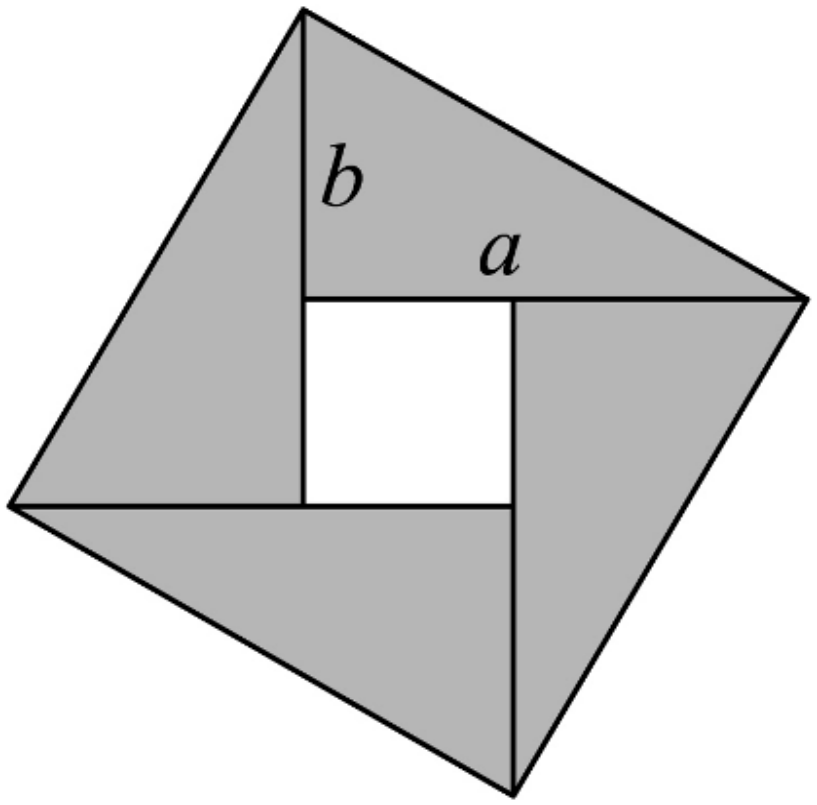
\includegraphics[width=0.20\textwidth]{figures/gao93_q16_zhaoshuang.png}
\end{center}

A. 如果 $a>b>0$，那么 $\sqrt a>\sqrt b$

B. 如果 $a>b>0$，那么 $a^2>b^2$

C. 对任意正实数 $a$ 和 $b$，有 $a^2+b^2\geqslant2ab$，当且仅当 $a=b$ 时等号成立

D. 对任意正实数 $a$ 和 $b$，有 $a^2+b^2\geqslant2ab$，当且仅当 $a=b$ 时等号成立% 原卷 C、D 两选项文字相同，照录

\ifanswer
\solbegin
\step{通过观察，可以发现这个图中的四个直角三角形是全等的，}
\step{设直角三角形的长直角边为 $a$，短直角边为 $b$，}
\step{如图，整个大正方形的面积大于等于这 $4$ 个直角三角形的面积和，}
\step{即 $a^2+b^2\geqslant4\times\left(\dfrac12ab\right)$，即 $a^2+b^2\geqslant2ab$，}
\step{当 $a=b$ 时，中间空白的正方形消失，即整个大正方形与 $4$ 个直角三角形重合；}
\step{其他选项通过该图无法证明. 故选 $C$.}
\solend
\fi

\end{enumerate}

\bigsec{三、解答题}

\begin{enumerate}
\setcounter{enumi}{16}

\item 已知 $x,y\in R$，比较 $x^2+y^2$ 与 $2(2x-y)-5$ 的大小.

\ansspace*[7]

\ifanswer
\solbegin
\step{因为 $x^2+y^2-2(2x-y)+5=(x-2)^2+(y+1)^2\geqslant0$，}
\step{所以 $x^2+y^2\geqslant2(2x-y)-5$.}
\solend
\fi

\item 设 $k\in\R$，求关于 $x$ 与 $y$ 的二元一次方程组 $\begin{cases}y=x+1\\ y=kx+3\end{cases}$ 的解集.

\ansspace*[9]

\ifanswer
\solbegin
\step{因为 $\begin{cases}y=x+1\\ y=kx+3\end{cases}$，两式相减，得到 $(k-1)x=-2$，}
\step{当 $k\neq1$ 时，$x=-\dfrac{2}{k-1}$，代入方程组中的第一式，得到 $y=\dfrac{k-3}{k-1}$，}
\step{此时，原方程组的解集为 $\left\{\left(-\dfrac{2}{k-1},\dfrac{k-3}{k-1}\right)\right\}$，}
\step{当 $k=1$ 时，方程 $(k-1)x=-2$ 无解，从而原方程组无解，其解集为空集.}
\step{综上，当 $k\neq1$ 时，解集为 $\left\{\left(-\dfrac{2}{k-1},\dfrac{k-3}{k-1}\right)\right\}$，}
\step{当 $k=1$ 时，解集为空集.}
\solend
\fi

\item 解下列不等式与方程组.

（1）解含绝对值的不等式：$\lvert x+1\rvert\geqslant3x$；

（2）求解不等式组 $\begin{cases}x^2-4x+3\geqslant0\\ \dfrac{x+3}{2x-1}\geqslant2\end{cases}$.

\ansspace*[10]

\ifanswer
\solbegin
\stepm{（1）}{当 $x\leqslant0$ 时，不等式显然成立，}
\step{当 $x>0$ 时，则 $(x+1)^2\geqslant9x^2$，得 $8x^2-2x-1\leqslant0$，}
\step{得 $(2x-1)(4x+1)\leqslant0$，解得 $-\dfrac14\leqslant x\leqslant\dfrac12$，由于 $x>0$，得 $0<x\leqslant\dfrac12$，}
\step{综上，不等式解集为 $\left\{x\left|x\leqslant\dfrac12\right.\right\}$.}
\stepm{（2）}{由 $x^2-4x+3\geqslant0$ 得 $(x-1)(x-3)\geqslant0$，所以 $x\leqslant1$ 或 $x\geqslant3$；}
\step{由 $\dfrac{x+3}{2x-1}\geqslant2$，得 $\dfrac{x+3}{2x-1}-2=\dfrac{-3x+5}{2x-1}\geqslant0$，即 $\dfrac{3x-5}{2x-1}\leqslant0$，}
\step{所以 $\begin{cases}(3x-5)(2x-1)\leqslant0\\ 2x-1\neq0\end{cases}$，解得 $\dfrac12<x\leqslant\dfrac53$，}
\step{所以不等式组的解集是 $\left\{x\left|\dfrac12<x\leqslant1\right.\right\}$.}
\solend
\fi

\item 已知关于 $x$ 的不等式 $2kx^2+kx-1<0$.

（1）若不等式的解集为 $\left(-\dfrac32,1\right)$，求实数 $k$ 的值；

（2）若不等式的解集为 $R$，求实数 $k$ 的取值范围.

\ansspace*[11]

\ifanswer
\solbegin
\stepm{（1）}{关于 $x$ 的不等式 $2kx^2+kx-1<0$ 的解集为 $\left(-\dfrac32,1\right)$，}
\step{所以 $-\dfrac32$ 和 $1$ 是方程 $2kx^2+kx-1=0$ 的两个实数根，}
\step{代入 $x=1$ 得 $2k+k-1=0$，解得 $k=\dfrac13$；}
\stepm{（2）}{若不等式 $2kx^2+kx-1<0$ 的解集为 $R$，}
\step{则 $k=0$ 时，不等式为 $-1<0$，满足题意；}
\step{$k\neq0$ 时，应满足 $\begin{cases}k<0\\ \Delta=k^2+8k<0\end{cases}$，解得 $-8<k<0$；}
\step{综上，实数 $k$ 的取值范围是 $-8<k\leqslant0$.}
\solend
\fi

\item 国家为了加强对烟酒生产的宏观管理，实行征收附加税政策，现知某种酒每瓶 $70$ 元，不征收附加税的时候，每年大约产销 $100$ 万瓶，若政府征收附加税，每销售 $100$ 元要征税 $R$ 元（叫做税率 $R\%$），则每年的销售将减少 $10R$ 万瓶.

（1）求出每年商店经营烟酒被征收的附加税税金 $S$（单位：万元）；

（2）若附加税税金 $S$ 不少于 $112$ 万元，且不大于 $168$ 万元，求 $R$ 的取值范围.

\ansspace*[12]

\ifanswer
\solbegin
\stepm{（1）}{由题意得 $S=70\times(100-10R)\times R\%(0\leqslant R\leqslant10)$（单位：万元）.}
\stepm{（2）}{由题意 $\begin{cases}70\times(100-10R)\times R\%\geqslant112\\ 70\times(100-10R)\times R\%\leqslant168\end{cases}$，解得 $2\leqslant R\leqslant4$ 或 $6\leqslant R\leqslant8$，}
\step{所以 $R$ 的取值范围是 $[2,4]\cup[6,8]$.}
\solend
\fi

\end{enumerate}

\end{document}
"
% 紧凑版：xelatex "\def\iscompact{1}% 高一93_建平世纪_10月月考.tex
%   —— 高一上数学“2026-2027 年建平世纪高一上 10 月月考”（讲评版）
% 试卷版：xelatex 高一93_建平世纪_10月月考.tex
% 答案版：xelatex "\def\isanswer{1}\input{高一93_建平世纪_10月月考.tex}"
% 紧凑版：xelatex "\def\iscompact{1}\input{高一93_建平世纪_10月月考.tex}"
%
% 原始材料：微信公众号“魔都数学加油站”文章，连载“27学年高一93”；
% 原文标题“27学年高一93——2026-2027年上海市建平世纪高一上10月月考”；
% 原文链接：https://mp.weixin.qq.com/s/uqySZX3I8Q-QZ2J8MqmWiA。
% 正文为 7 张 PNG 页（`原图/高一93_建平世纪_10月月考/01..07.png`），均 4762×6735，按页序读取。
%
% 篇幅与题号：原卷自第 3 题起编号（第 1、2 题不在原文内）。填空题 3—12（10 题）、
% 选择题 13—16（4 题）、解答题 17—21（5 题），共 19 题。
%
% 讲评版：第 3、4 题只印【答案】（“$\{x\mid-1<x<1\}$”“$x$ 和 $y$ 不都是有理数”），本稿只给 \ans{}；
% 其余 17 题印【解析】，其中选择题答案在解析末句“故选 $D$／$D$／$C$／$C$”。
% 第 16 题题干右侧有一幅赵爽弦图（裁自第 4 页原图、去粉色水印后转灰度）。
%
% 副标题：原卷未印副标题。本稿按内容标作“集合与常用逻辑用语、不等式”。
%
% 原卷笔误/存疑（均照录未改，正文对应处另有 % 注）：
%   ① 第 3 题答案印作 $\{x\mid-1<x<1\}$（两端开），而 $\lvert x\rvert\leqslant1$ 的解集应为
%      $[-1,1]$（两端闭）；原卷照录，未改；
%   ② 第 16 题 C、D 两个选项**文字完全相同**（皆为“对任意正实数 $a$ 和 $b$，有
%      $a^2+b^2\geqslant2ab$，当且仅当 $a=b$ 时等号成立”），原卷重复排印；答案取 $C$，
%      本稿两个选项照录。
%
% 与原卷的排版差异：
%   ① 原卷每题下直接印【答案】/【解析】，本稿按全稿惯例将答案与解析置于答案版；
%   ② 原卷未印副标题，本稿补出；填空横线统一排 \blankline[4.4em]；
%   ③ 原卷数集记号排斜体 $R$，本稿按全稿惯例改用 $\R$；
%   ④ 第 17—21 题的子问用行内“（1）（2）（3）”段，解析中的子问标号用 \stepm；
%   ⑤ 解答题按惯例加 \ansspace；选择题括号排 \mbox{（\quad）}；
%   ⑥ 第 16 题的弦图原卷排在题干右侧、文字绕排，本稿改排为选项后的居中图。
%
% 行数核对：逐题数 \step/\stepm 条数，合计 71 条（Q3：0；Q4：0；Q5：2；Q6：3；Q7：2；
% Q8：2；Q9：4；Q10：1；Q11：3；Q12：9；Q13：5；Q14：3；Q15：5；Q16：6；Q17：2；
% Q18：6；Q19：8；Q20：7；Q21：3）。第 3、4 题只印答案，不计入 \step 账。
% 原卷解析的换行按语意合并，未逐行强拆。
%
\documentclass[a4paper,11pt]{article}
\usepackage{common}

\begin{document}

\examtitlest[7]{2026--2027 年建平世纪高一上 10 月月考}{集合与常用逻辑用语、不等式}

\bigsec{一、填空题}

\begin{enumerate}
\setcounter{enumi}{2}

\item 不等式 $\lvert x\rvert\leqslant1$ 的解集是\blankline[4.4em].

\ifanswer
\ans{$\{x\mid-1<x<1\}$}% 原卷答案两端开；|x|≤1 应为 [-1,1]，照录
\fi

\item “$x$ 和 $y$ 都是有理数”的否定形式是\blankline[4.4em].

\ifanswer
\ans{$x$ 和 $y$ 不都是有理数}
\fi

\item 已知等式 $2x^2+3x+5=2ax^2+a(3x+1)+c$ 恒成立，则 $a+c=\blankline[4.4em]$.

\ifanswer
\solbegin
\step{因为 $2x^2+3x+5=2ax^2+a(3x+1)+c$ 恒成立，}
\step{即 $2x^2+3x+5=2ax^2+3ax+(a+c)$ 恒成立，所以 $\begin{cases}2=2a\\ 3=3a\\ 5=a+c\end{cases}$，所以 $a+c=5$.}
\solend
\fi

\item 已知方程 $x^2+6x+m=0(m\in\R)$ 的两个根 $x_1$、$x_2$ 满足 $\lvert x_1-x_2\rvert=4$，则 $m$ 的值是\blankline[4.4em].

\ifanswer
\solbegin
\step{方程 $x^2+6x+m=0(m\in\R)$ 的两根为 $x_1$、$x_2$，所以 $x_1+x_2=-6$，$x_1x_2=m$，}
\step{又 $\lvert x_1-x_2\rvert=4$，则 $(x_1-x_2)^2=(x_1+x_2)^2-4x_1x_2=16$，}
\step{即 $(-6)^2-4m=16$，解得 $m=5$，检验得 $\Delta=6^2-4\times1\times5=16>0$，符合题意，所以 $m=5$.}
\solend
\fi

\item 已知 $\alpha:2m-6<x<m+5$，$\beta:-3<x<5$，若 $\alpha$ 是 $\beta$ 的必要条件，则实数 $m$ 的取值范围是\blankline[4.4em].

\ifanswer
\solbegin
\step{因为 $\alpha$ 是 $\beta$ 的必要条件，所以 $\begin{cases}2m-6\leqslant-3\\ m+5\geqslant5\\ 2m-6<m+5\end{cases}\Rightarrow0\leqslant m\leqslant\dfrac32$，}
\step{所以实数 $m$ 的取值范围是 $\left[0,\dfrac32\right]$.}
\solend
\fi

\item 已知 $-2\leqslant a\leqslant3$，$2\leqslant b\leqslant\dfrac72$，则 $a-2b$ 的取值范围为\blankline[4.4em].

\ifanswer
\solbegin
\step{因为 $-2\leqslant a\leqslant3$，$2\leqslant b\leqslant\dfrac72$，所以 $-7\leqslant-2b\leqslant-4$，所以 $-9\leqslant a-2b\leqslant-1$，}
\step{故 $a-2b$ 的取值范围为 $[-9,-1]$.}
\solend
\fi

\item 已知 $\lvert x+3\rvert+\lvert5-x\rvert>10$，则实数 $x$ 的取值范围为\blankline[4.4em].

\ifanswer
\solbegin
\step{当 $x<-3$ 时，则 $-x-3+5-x>10$，解得 $x<-4$，}
\step{当 $-3\leqslant x\leqslant5$ 时，则 $x+3+5-x=8<10$，原不等式不成立，}
\step{当 $x>5$ 时，则 $x+3+x-5>10$，解得 $x>6$，}
\step{综上所述，实数 $x$ 的取值范围为 $(-\infty,-4)\cup(6,+\infty)$.}
\solend
\fi

\item 已知集合 $A=\{(x,y)\mid y=x+1\}$，$B=\{(x,y)\mid y=-x+3\}$，则 $A\cap B=\blankline[4.4em]$.

\ifanswer
\solbegin
\step{联立 $\begin{cases}y=x+1\\ y=-x+3\end{cases}$，解得 $x=1$，$y=2$，故 $A\cap B=\{(1,2)\}$.}
\solend
\fi

\item 若关于 $x$ 的不等式组 $\begin{cases}\dfrac{x-1}{x-3}<0\\ x>a\end{cases}$ 的解集为空集，则实数 $a$ 的取值范围为\blankline[4.4em].

\ifanswer
\solbegin
\step{$\dfrac{x-1}{x-3}<0$ 等价于 $(x-1)(x-3)<0$，得 $1<x<3$，}
\step{因为 $\begin{cases}\dfrac{x-1}{x-3}<0\\ x>a\end{cases}$ 的解集为空集，}
\step{所以 $a\geqslant3$，故实数 $a$ 的取值范围为 $[3,+\infty)$.}
\solend
\fi

\item 已知由自然数组成的 $n-1$ 个元素的集合 $A=\{1,2,3,4,\cdots,n-1\}(n>1)$，非空集合 $B\subseteq A$，且对任意的 $a\in B$，都有 $n-a\in B$. 当 $n=9$ 时，则所有满足条件的集合 $B$ 的元素的和为\blankline[4.4em].

\ifanswer
\solbegin
\step{当 $n=9$ 时，$A=\{1,2,3,4,5,6,7,8\}$，}
\step{当 $B$ 中有两个元素时，集合 $B$ 可以为 $\{1,8\},\{2,7\},\{3,6\},\{4,5\}$，}
\step{元素总和为 $4\times9=36$；}
\step{当 $B$ 中有四个元素时，集合 $B$ 可以为 $\{1,8\},\{2,7\},\{3,6\},\{4,5\}$ 中任取两个的并集，}
\step{集合 $B$ 共有 $6$ 种情况，元素总和为 $6\times2\times9=108$；}
\step{当 $B$ 中有六个元素时，集合 $B$ 可以为 $\{1,8\},\{2,7\},\{3,6\},\{4,5\}$ 中任取三个的并集，}
\step{集合 $B$ 共有 $4$ 种情况，元素总和为 $4\times3\times9=12\times9=108$；}
\step{当 $B$ 中有八个元素时，$B=\{1,2,3,4,5,6,7,8\}$，元素之和为 $4\times9=36$，}
\step{所以所有满足条件的集合 $B$ 的元素总和为 $36+108+108+36=288$.}
\solend
\fi

\end{enumerate}

\bigsec{二、选择题}

\begin{enumerate}
\setcounter{enumi}{12}

\item 下列说法正确的是\mbox{（\quad）}

\keepwithprev
A. 若 $a>b$，则 $\dfrac1a<\dfrac1b$\qquad B. 若 $a>b,c>d$，则 $ac>bd$

C. 若 $a>b$，则 $ac^2>bc^2$\qquad D. 若 $ac^2>bc^2$，则 $a>b$

\ifanswer
\solbegin
\step{A：令 $a=2,b=-1$，此时 $\dfrac12>-1$，故 A 错误；}
\step{B：令 $a=2,b=-1,c=0,d=-2$，此时 $ac=0<bd=2$，故 B 错误；}
\step{C：由 $a>b$，当 $c=0$ 时，$ac^2=bc^2$，故 C 错误；}
\step{D：由 $ac^2>bc^2$，则 $c^2>0$，所以 $a>b$，故 D 正确.}
\step{故选 $D$.}
\solend
\fi

\item 不等式 $\dfrac{x-3}{x-1}\leqslant2$ 的解集是\mbox{（\quad）}

\keepwithprev
A. $(-\infty,1]$\qquad B. $[1,+\infty)$

C. $(-\infty,-1]\cup[1,+\infty)$\qquad D. $(-\infty,-1]\cup(1,+\infty)$

\ifanswer
\solbegin
\step{不等式 $\dfrac{x-3}{x-1}\leqslant2$ 可化为 $\dfrac{x-3}{x-1}-2\leqslant0$，即 $\dfrac{x-3-2(x-1)}{x-1}\leqslant0$，}
\step{化简得 $\dfrac{x+1}{x-1}\geqslant0$，等价于 $\begin{cases}(x+1)(x-1)\geqslant0\\ x\neq1\end{cases}$，解得 $x\leqslant-1$ 或 $x>1$，}
\step{所以不等式的解集为 $(-\infty,-1]\cup(1,+\infty)$. 故选 $D$.}
\solend
\fi

\item 已知集合 $M$ 和集合 $N$，那么 $M\cap N=N$ 的充要条件是\mbox{（\quad）}

\keepwithprev
A. $M\subseteq N$\qquad B. $N\subset M$\qquad C. $M\supseteq N$\qquad D. $M=N$

\ifanswer
\solbegin
\step{若 $M\subseteq N$，即集合 $M$ 是集合 $N$ 的子集，则 $M\cap N=M$，故 $A$ 错误；}
\step{若 $M=N$，则不能得到 $N\subset M$，故 $B$ 错误；}
\step{若 $M\cap N=N$，则 $M\supseteq N$，故 $C$ 正确；}
\step{当 $N$ 是 $M$ 真子集时，不能得到 $M=N$，故 $D$ 错误.}
\step{故选 $C$.}
\solend
\fi

\item 三国时期赵爽在《勾股方圆图注》中对勾股定理的证明可用现代数学表述为如图所示，我们教材中利用该图作为“（\quad）”的几何解释.

\begin{center}
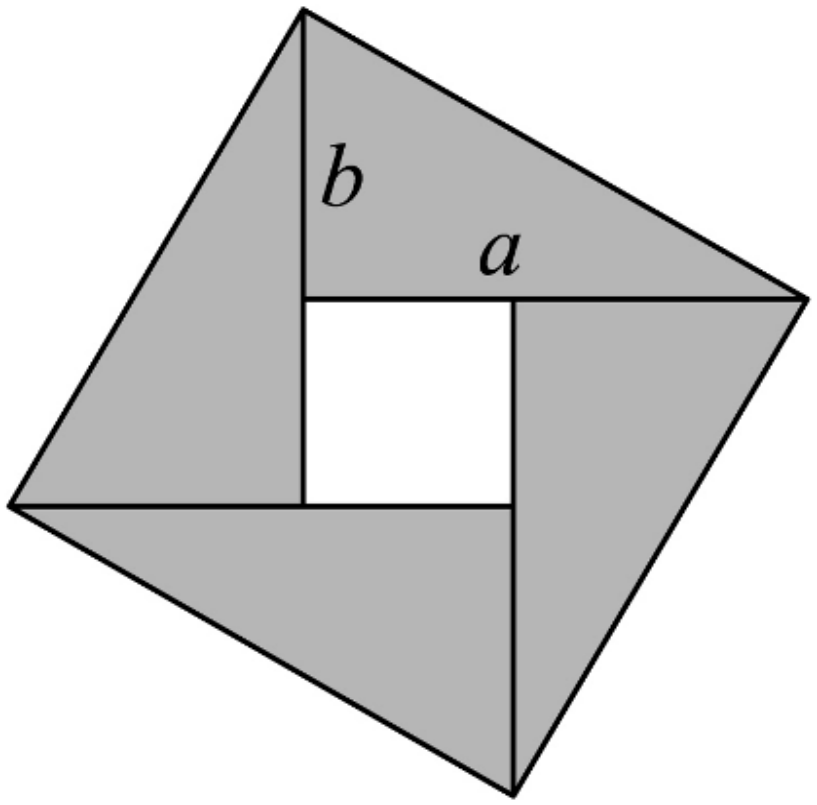
\includegraphics[width=0.20\textwidth]{figures/gao93_q16_zhaoshuang.png}
\end{center}

A. 如果 $a>b>0$，那么 $\sqrt a>\sqrt b$

B. 如果 $a>b>0$，那么 $a^2>b^2$

C. 对任意正实数 $a$ 和 $b$，有 $a^2+b^2\geqslant2ab$，当且仅当 $a=b$ 时等号成立

D. 对任意正实数 $a$ 和 $b$，有 $a^2+b^2\geqslant2ab$，当且仅当 $a=b$ 时等号成立% 原卷 C、D 两选项文字相同，照录

\ifanswer
\solbegin
\step{通过观察，可以发现这个图中的四个直角三角形是全等的，}
\step{设直角三角形的长直角边为 $a$，短直角边为 $b$，}
\step{如图，整个大正方形的面积大于等于这 $4$ 个直角三角形的面积和，}
\step{即 $a^2+b^2\geqslant4\times\left(\dfrac12ab\right)$，即 $a^2+b^2\geqslant2ab$，}
\step{当 $a=b$ 时，中间空白的正方形消失，即整个大正方形与 $4$ 个直角三角形重合；}
\step{其他选项通过该图无法证明. 故选 $C$.}
\solend
\fi

\end{enumerate}

\bigsec{三、解答题}

\begin{enumerate}
\setcounter{enumi}{16}

\item 已知 $x,y\in R$，比较 $x^2+y^2$ 与 $2(2x-y)-5$ 的大小.

\ansspace*[7]

\ifanswer
\solbegin
\step{因为 $x^2+y^2-2(2x-y)+5=(x-2)^2+(y+1)^2\geqslant0$，}
\step{所以 $x^2+y^2\geqslant2(2x-y)-5$.}
\solend
\fi

\item 设 $k\in\R$，求关于 $x$ 与 $y$ 的二元一次方程组 $\begin{cases}y=x+1\\ y=kx+3\end{cases}$ 的解集.

\ansspace*[9]

\ifanswer
\solbegin
\step{因为 $\begin{cases}y=x+1\\ y=kx+3\end{cases}$，两式相减，得到 $(k-1)x=-2$，}
\step{当 $k\neq1$ 时，$x=-\dfrac{2}{k-1}$，代入方程组中的第一式，得到 $y=\dfrac{k-3}{k-1}$，}
\step{此时，原方程组的解集为 $\left\{\left(-\dfrac{2}{k-1},\dfrac{k-3}{k-1}\right)\right\}$，}
\step{当 $k=1$ 时，方程 $(k-1)x=-2$ 无解，从而原方程组无解，其解集为空集.}
\step{综上，当 $k\neq1$ 时，解集为 $\left\{\left(-\dfrac{2}{k-1},\dfrac{k-3}{k-1}\right)\right\}$，}
\step{当 $k=1$ 时，解集为空集.}
\solend
\fi

\item 解下列不等式与方程组.

（1）解含绝对值的不等式：$\lvert x+1\rvert\geqslant3x$；

（2）求解不等式组 $\begin{cases}x^2-4x+3\geqslant0\\ \dfrac{x+3}{2x-1}\geqslant2\end{cases}$.

\ansspace*[10]

\ifanswer
\solbegin
\stepm{（1）}{当 $x\leqslant0$ 时，不等式显然成立，}
\step{当 $x>0$ 时，则 $(x+1)^2\geqslant9x^2$，得 $8x^2-2x-1\leqslant0$，}
\step{得 $(2x-1)(4x+1)\leqslant0$，解得 $-\dfrac14\leqslant x\leqslant\dfrac12$，由于 $x>0$，得 $0<x\leqslant\dfrac12$，}
\step{综上，不等式解集为 $\left\{x\left|x\leqslant\dfrac12\right.\right\}$.}
\stepm{（2）}{由 $x^2-4x+3\geqslant0$ 得 $(x-1)(x-3)\geqslant0$，所以 $x\leqslant1$ 或 $x\geqslant3$；}
\step{由 $\dfrac{x+3}{2x-1}\geqslant2$，得 $\dfrac{x+3}{2x-1}-2=\dfrac{-3x+5}{2x-1}\geqslant0$，即 $\dfrac{3x-5}{2x-1}\leqslant0$，}
\step{所以 $\begin{cases}(3x-5)(2x-1)\leqslant0\\ 2x-1\neq0\end{cases}$，解得 $\dfrac12<x\leqslant\dfrac53$，}
\step{所以不等式组的解集是 $\left\{x\left|\dfrac12<x\leqslant1\right.\right\}$.}
\solend
\fi

\item 已知关于 $x$ 的不等式 $2kx^2+kx-1<0$.

（1）若不等式的解集为 $\left(-\dfrac32,1\right)$，求实数 $k$ 的值；

（2）若不等式的解集为 $R$，求实数 $k$ 的取值范围.

\ansspace*[11]

\ifanswer
\solbegin
\stepm{（1）}{关于 $x$ 的不等式 $2kx^2+kx-1<0$ 的解集为 $\left(-\dfrac32,1\right)$，}
\step{所以 $-\dfrac32$ 和 $1$ 是方程 $2kx^2+kx-1=0$ 的两个实数根，}
\step{代入 $x=1$ 得 $2k+k-1=0$，解得 $k=\dfrac13$；}
\stepm{（2）}{若不等式 $2kx^2+kx-1<0$ 的解集为 $R$，}
\step{则 $k=0$ 时，不等式为 $-1<0$，满足题意；}
\step{$k\neq0$ 时，应满足 $\begin{cases}k<0\\ \Delta=k^2+8k<0\end{cases}$，解得 $-8<k<0$；}
\step{综上，实数 $k$ 的取值范围是 $-8<k\leqslant0$.}
\solend
\fi

\item 国家为了加强对烟酒生产的宏观管理，实行征收附加税政策，现知某种酒每瓶 $70$ 元，不征收附加税的时候，每年大约产销 $100$ 万瓶，若政府征收附加税，每销售 $100$ 元要征税 $R$ 元（叫做税率 $R\%$），则每年的销售将减少 $10R$ 万瓶.

（1）求出每年商店经营烟酒被征收的附加税税金 $S$（单位：万元）；

（2）若附加税税金 $S$ 不少于 $112$ 万元，且不大于 $168$ 万元，求 $R$ 的取值范围.

\ansspace*[12]

\ifanswer
\solbegin
\stepm{（1）}{由题意得 $S=70\times(100-10R)\times R\%(0\leqslant R\leqslant10)$（单位：万元）.}
\stepm{（2）}{由题意 $\begin{cases}70\times(100-10R)\times R\%\geqslant112\\ 70\times(100-10R)\times R\%\leqslant168\end{cases}$，解得 $2\leqslant R\leqslant4$ 或 $6\leqslant R\leqslant8$，}
\step{所以 $R$ 的取值范围是 $[2,4]\cup[6,8]$.}
\solend
\fi

\end{enumerate}

\end{document}
"
%
% 原始材料：微信公众号“魔都数学加油站”文章，连载“27学年高一93”；
% 原文标题“27学年高一93——2026-2027年上海市建平世纪高一上10月月考”；
% 原文链接：https://mp.weixin.qq.com/s/uqySZX3I8Q-QZ2J8MqmWiA。
% 正文为 7 张 PNG 页（`原图/高一93_建平世纪_10月月考/01..07.png`），均 4762×6735，按页序读取。
%
% 篇幅与题号：原卷自第 3 题起编号（第 1、2 题不在原文内）。填空题 3—12（10 题）、
% 选择题 13—16（4 题）、解答题 17—21（5 题），共 19 题。
%
% 讲评版：第 3、4 题只印【答案】（“$\{x\mid-1<x<1\}$”“$x$ 和 $y$ 不都是有理数”），本稿只给 \ans{}；
% 其余 17 题印【解析】，其中选择题答案在解析末句“故选 $D$／$D$／$C$／$C$”。
% 第 16 题题干右侧有一幅赵爽弦图（裁自第 4 页原图、去粉色水印后转灰度）。
%
% 副标题：原卷未印副标题。本稿按内容标作“集合与常用逻辑用语、不等式”。
%
% 原卷笔误/存疑（均照录未改，正文对应处另有 % 注）：
%   ① 第 3 题答案印作 $\{x\mid-1<x<1\}$（两端开），而 $\lvert x\rvert\leqslant1$ 的解集应为
%      $[-1,1]$（两端闭）；原卷照录，未改；
%   ② 第 16 题 C、D 两个选项**文字完全相同**（皆为“对任意正实数 $a$ 和 $b$，有
%      $a^2+b^2\geqslant2ab$，当且仅当 $a=b$ 时等号成立”），原卷重复排印；答案取 $C$，
%      本稿两个选项照录。
%
% 与原卷的排版差异：
%   ① 原卷每题下直接印【答案】/【解析】，本稿按全稿惯例将答案与解析置于答案版；
%   ② 原卷未印副标题，本稿补出；填空横线统一排 \blankline[4.4em]；
%   ③ 原卷数集记号排斜体 $R$，本稿按全稿惯例改用 $\R$；
%   ④ 第 17—21 题的子问用行内“（1）（2）（3）”段，解析中的子问标号用 \stepm；
%   ⑤ 解答题按惯例加 \ansspace；选择题括号排 \mbox{（\quad）}；
%   ⑥ 第 16 题的弦图原卷排在题干右侧、文字绕排，本稿改排为选项后的居中图。
%
% 行数核对：逐题数 \step/\stepm 条数，合计 71 条（Q3：0；Q4：0；Q5：2；Q6：3；Q7：2；
% Q8：2；Q9：4；Q10：1；Q11：3；Q12：9；Q13：5；Q14：3；Q15：5；Q16：6；Q17：2；
% Q18：6；Q19：8；Q20：7；Q21：3）。第 3、4 题只印答案，不计入 \step 账。
% 原卷解析的换行按语意合并，未逐行强拆。
%
\documentclass[a4paper,11pt]{article}
\usepackage{common}

\begin{document}

\examtitlest[7]{2026--2027 年建平世纪高一上 10 月月考}{集合与常用逻辑用语、不等式}

\bigsec{一、填空题}

\begin{enumerate}
\setcounter{enumi}{2}

\item 不等式 $\lvert x\rvert\leqslant1$ 的解集是\blankline[4.4em].

\ifanswer
\ans{$\{x\mid-1<x<1\}$}% 原卷答案两端开；|x|≤1 应为 [-1,1]，照录
\fi

\item “$x$ 和 $y$ 都是有理数”的否定形式是\blankline[4.4em].

\ifanswer
\ans{$x$ 和 $y$ 不都是有理数}
\fi

\item 已知等式 $2x^2+3x+5=2ax^2+a(3x+1)+c$ 恒成立，则 $a+c=\blankline[4.4em]$.

\ifanswer
\solbegin
\step{因为 $2x^2+3x+5=2ax^2+a(3x+1)+c$ 恒成立，}
\step{即 $2x^2+3x+5=2ax^2+3ax+(a+c)$ 恒成立，所以 $\begin{cases}2=2a\\ 3=3a\\ 5=a+c\end{cases}$，所以 $a+c=5$.}
\solend
\fi

\item 已知方程 $x^2+6x+m=0(m\in\R)$ 的两个根 $x_1$、$x_2$ 满足 $\lvert x_1-x_2\rvert=4$，则 $m$ 的值是\blankline[4.4em].

\ifanswer
\solbegin
\step{方程 $x^2+6x+m=0(m\in\R)$ 的两根为 $x_1$、$x_2$，所以 $x_1+x_2=-6$，$x_1x_2=m$，}
\step{又 $\lvert x_1-x_2\rvert=4$，则 $(x_1-x_2)^2=(x_1+x_2)^2-4x_1x_2=16$，}
\step{即 $(-6)^2-4m=16$，解得 $m=5$，检验得 $\Delta=6^2-4\times1\times5=16>0$，符合题意，所以 $m=5$.}
\solend
\fi

\item 已知 $\alpha:2m-6<x<m+5$，$\beta:-3<x<5$，若 $\alpha$ 是 $\beta$ 的必要条件，则实数 $m$ 的取值范围是\blankline[4.4em].

\ifanswer
\solbegin
\step{因为 $\alpha$ 是 $\beta$ 的必要条件，所以 $\begin{cases}2m-6\leqslant-3\\ m+5\geqslant5\\ 2m-6<m+5\end{cases}\Rightarrow0\leqslant m\leqslant\dfrac32$，}
\step{所以实数 $m$ 的取值范围是 $\left[0,\dfrac32\right]$.}
\solend
\fi

\item 已知 $-2\leqslant a\leqslant3$，$2\leqslant b\leqslant\dfrac72$，则 $a-2b$ 的取值范围为\blankline[4.4em].

\ifanswer
\solbegin
\step{因为 $-2\leqslant a\leqslant3$，$2\leqslant b\leqslant\dfrac72$，所以 $-7\leqslant-2b\leqslant-4$，所以 $-9\leqslant a-2b\leqslant-1$，}
\step{故 $a-2b$ 的取值范围为 $[-9,-1]$.}
\solend
\fi

\item 已知 $\lvert x+3\rvert+\lvert5-x\rvert>10$，则实数 $x$ 的取值范围为\blankline[4.4em].

\ifanswer
\solbegin
\step{当 $x<-3$ 时，则 $-x-3+5-x>10$，解得 $x<-4$，}
\step{当 $-3\leqslant x\leqslant5$ 时，则 $x+3+5-x=8<10$，原不等式不成立，}
\step{当 $x>5$ 时，则 $x+3+x-5>10$，解得 $x>6$，}
\step{综上所述，实数 $x$ 的取值范围为 $(-\infty,-4)\cup(6,+\infty)$.}
\solend
\fi

\item 已知集合 $A=\{(x,y)\mid y=x+1\}$，$B=\{(x,y)\mid y=-x+3\}$，则 $A\cap B=\blankline[4.4em]$.

\ifanswer
\solbegin
\step{联立 $\begin{cases}y=x+1\\ y=-x+3\end{cases}$，解得 $x=1$，$y=2$，故 $A\cap B=\{(1,2)\}$.}
\solend
\fi

\item 若关于 $x$ 的不等式组 $\begin{cases}\dfrac{x-1}{x-3}<0\\ x>a\end{cases}$ 的解集为空集，则实数 $a$ 的取值范围为\blankline[4.4em].

\ifanswer
\solbegin
\step{$\dfrac{x-1}{x-3}<0$ 等价于 $(x-1)(x-3)<0$，得 $1<x<3$，}
\step{因为 $\begin{cases}\dfrac{x-1}{x-3}<0\\ x>a\end{cases}$ 的解集为空集，}
\step{所以 $a\geqslant3$，故实数 $a$ 的取值范围为 $[3,+\infty)$.}
\solend
\fi

\item 已知由自然数组成的 $n-1$ 个元素的集合 $A=\{1,2,3,4,\cdots,n-1\}(n>1)$，非空集合 $B\subseteq A$，且对任意的 $a\in B$，都有 $n-a\in B$. 当 $n=9$ 时，则所有满足条件的集合 $B$ 的元素的和为\blankline[4.4em].

\ifanswer
\solbegin
\step{当 $n=9$ 时，$A=\{1,2,3,4,5,6,7,8\}$，}
\step{当 $B$ 中有两个元素时，集合 $B$ 可以为 $\{1,8\},\{2,7\},\{3,6\},\{4,5\}$，}
\step{元素总和为 $4\times9=36$；}
\step{当 $B$ 中有四个元素时，集合 $B$ 可以为 $\{1,8\},\{2,7\},\{3,6\},\{4,5\}$ 中任取两个的并集，}
\step{集合 $B$ 共有 $6$ 种情况，元素总和为 $6\times2\times9=108$；}
\step{当 $B$ 中有六个元素时，集合 $B$ 可以为 $\{1,8\},\{2,7\},\{3,6\},\{4,5\}$ 中任取三个的并集，}
\step{集合 $B$ 共有 $4$ 种情况，元素总和为 $4\times3\times9=12\times9=108$；}
\step{当 $B$ 中有八个元素时，$B=\{1,2,3,4,5,6,7,8\}$，元素之和为 $4\times9=36$，}
\step{所以所有满足条件的集合 $B$ 的元素总和为 $36+108+108+36=288$.}
\solend
\fi

\end{enumerate}

\bigsec{二、选择题}

\begin{enumerate}
\setcounter{enumi}{12}

\item 下列说法正确的是\mbox{（\quad）}

\keepwithprev
A. 若 $a>b$，则 $\dfrac1a<\dfrac1b$\qquad B. 若 $a>b,c>d$，则 $ac>bd$

C. 若 $a>b$，则 $ac^2>bc^2$\qquad D. 若 $ac^2>bc^2$，则 $a>b$

\ifanswer
\solbegin
\step{A：令 $a=2,b=-1$，此时 $\dfrac12>-1$，故 A 错误；}
\step{B：令 $a=2,b=-1,c=0,d=-2$，此时 $ac=0<bd=2$，故 B 错误；}
\step{C：由 $a>b$，当 $c=0$ 时，$ac^2=bc^2$，故 C 错误；}
\step{D：由 $ac^2>bc^2$，则 $c^2>0$，所以 $a>b$，故 D 正确.}
\step{故选 $D$.}
\solend
\fi

\item 不等式 $\dfrac{x-3}{x-1}\leqslant2$ 的解集是\mbox{（\quad）}

\keepwithprev
A. $(-\infty,1]$\qquad B. $[1,+\infty)$

C. $(-\infty,-1]\cup[1,+\infty)$\qquad D. $(-\infty,-1]\cup(1,+\infty)$

\ifanswer
\solbegin
\step{不等式 $\dfrac{x-3}{x-1}\leqslant2$ 可化为 $\dfrac{x-3}{x-1}-2\leqslant0$，即 $\dfrac{x-3-2(x-1)}{x-1}\leqslant0$，}
\step{化简得 $\dfrac{x+1}{x-1}\geqslant0$，等价于 $\begin{cases}(x+1)(x-1)\geqslant0\\ x\neq1\end{cases}$，解得 $x\leqslant-1$ 或 $x>1$，}
\step{所以不等式的解集为 $(-\infty,-1]\cup(1,+\infty)$. 故选 $D$.}
\solend
\fi

\item 已知集合 $M$ 和集合 $N$，那么 $M\cap N=N$ 的充要条件是\mbox{（\quad）}

\keepwithprev
A. $M\subseteq N$\qquad B. $N\subset M$\qquad C. $M\supseteq N$\qquad D. $M=N$

\ifanswer
\solbegin
\step{若 $M\subseteq N$，即集合 $M$ 是集合 $N$ 的子集，则 $M\cap N=M$，故 $A$ 错误；}
\step{若 $M=N$，则不能得到 $N\subset M$，故 $B$ 错误；}
\step{若 $M\cap N=N$，则 $M\supseteq N$，故 $C$ 正确；}
\step{当 $N$ 是 $M$ 真子集时，不能得到 $M=N$，故 $D$ 错误.}
\step{故选 $C$.}
\solend
\fi

\item 三国时期赵爽在《勾股方圆图注》中对勾股定理的证明可用现代数学表述为如图所示，我们教材中利用该图作为“（\quad）”的几何解释.

\begin{center}
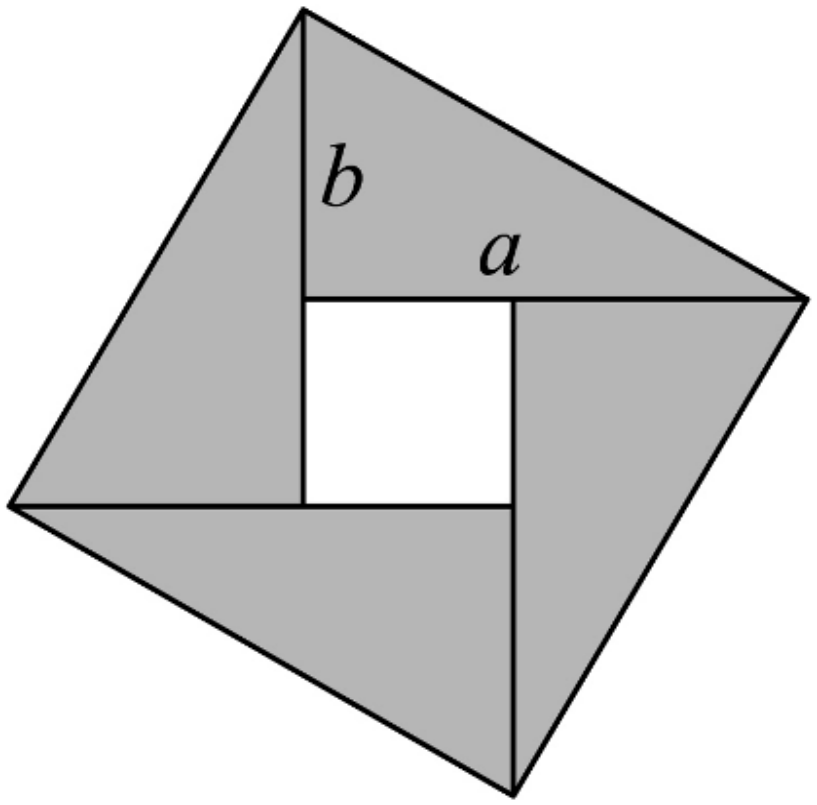
\includegraphics[width=0.20\textwidth]{figures/gao93_q16_zhaoshuang.png}
\end{center}

A. 如果 $a>b>0$，那么 $\sqrt a>\sqrt b$

B. 如果 $a>b>0$，那么 $a^2>b^2$

C. 对任意正实数 $a$ 和 $b$，有 $a^2+b^2\geqslant2ab$，当且仅当 $a=b$ 时等号成立

D. 对任意正实数 $a$ 和 $b$，有 $a^2+b^2\geqslant2ab$，当且仅当 $a=b$ 时等号成立% 原卷 C、D 两选项文字相同，照录

\ifanswer
\solbegin
\step{通过观察，可以发现这个图中的四个直角三角形是全等的，}
\step{设直角三角形的长直角边为 $a$，短直角边为 $b$，}
\step{如图，整个大正方形的面积大于等于这 $4$ 个直角三角形的面积和，}
\step{即 $a^2+b^2\geqslant4\times\left(\dfrac12ab\right)$，即 $a^2+b^2\geqslant2ab$，}
\step{当 $a=b$ 时，中间空白的正方形消失，即整个大正方形与 $4$ 个直角三角形重合；}
\step{其他选项通过该图无法证明. 故选 $C$.}
\solend
\fi

\end{enumerate}

\bigsec{三、解答题}

\begin{enumerate}
\setcounter{enumi}{16}

\item 已知 $x,y\in R$，比较 $x^2+y^2$ 与 $2(2x-y)-5$ 的大小.

\ansspace*[7]

\ifanswer
\solbegin
\step{因为 $x^2+y^2-2(2x-y)+5=(x-2)^2+(y+1)^2\geqslant0$，}
\step{所以 $x^2+y^2\geqslant2(2x-y)-5$.}
\solend
\fi

\item 设 $k\in\R$，求关于 $x$ 与 $y$ 的二元一次方程组 $\begin{cases}y=x+1\\ y=kx+3\end{cases}$ 的解集.

\ansspace*[9]

\ifanswer
\solbegin
\step{因为 $\begin{cases}y=x+1\\ y=kx+3\end{cases}$，两式相减，得到 $(k-1)x=-2$，}
\step{当 $k\neq1$ 时，$x=-\dfrac{2}{k-1}$，代入方程组中的第一式，得到 $y=\dfrac{k-3}{k-1}$，}
\step{此时，原方程组的解集为 $\left\{\left(-\dfrac{2}{k-1},\dfrac{k-3}{k-1}\right)\right\}$，}
\step{当 $k=1$ 时，方程 $(k-1)x=-2$ 无解，从而原方程组无解，其解集为空集.}
\step{综上，当 $k\neq1$ 时，解集为 $\left\{\left(-\dfrac{2}{k-1},\dfrac{k-3}{k-1}\right)\right\}$，}
\step{当 $k=1$ 时，解集为空集.}
\solend
\fi

\item 解下列不等式与方程组.

（1）解含绝对值的不等式：$\lvert x+1\rvert\geqslant3x$；

（2）求解不等式组 $\begin{cases}x^2-4x+3\geqslant0\\ \dfrac{x+3}{2x-1}\geqslant2\end{cases}$.

\ansspace*[10]

\ifanswer
\solbegin
\stepm{（1）}{当 $x\leqslant0$ 时，不等式显然成立，}
\step{当 $x>0$ 时，则 $(x+1)^2\geqslant9x^2$，得 $8x^2-2x-1\leqslant0$，}
\step{得 $(2x-1)(4x+1)\leqslant0$，解得 $-\dfrac14\leqslant x\leqslant\dfrac12$，由于 $x>0$，得 $0<x\leqslant\dfrac12$，}
\step{综上，不等式解集为 $\left\{x\left|x\leqslant\dfrac12\right.\right\}$.}
\stepm{（2）}{由 $x^2-4x+3\geqslant0$ 得 $(x-1)(x-3)\geqslant0$，所以 $x\leqslant1$ 或 $x\geqslant3$；}
\step{由 $\dfrac{x+3}{2x-1}\geqslant2$，得 $\dfrac{x+3}{2x-1}-2=\dfrac{-3x+5}{2x-1}\geqslant0$，即 $\dfrac{3x-5}{2x-1}\leqslant0$，}
\step{所以 $\begin{cases}(3x-5)(2x-1)\leqslant0\\ 2x-1\neq0\end{cases}$，解得 $\dfrac12<x\leqslant\dfrac53$，}
\step{所以不等式组的解集是 $\left\{x\left|\dfrac12<x\leqslant1\right.\right\}$.}
\solend
\fi

\item 已知关于 $x$ 的不等式 $2kx^2+kx-1<0$.

（1）若不等式的解集为 $\left(-\dfrac32,1\right)$，求实数 $k$ 的值；

（2）若不等式的解集为 $R$，求实数 $k$ 的取值范围.

\ansspace*[11]

\ifanswer
\solbegin
\stepm{（1）}{关于 $x$ 的不等式 $2kx^2+kx-1<0$ 的解集为 $\left(-\dfrac32,1\right)$，}
\step{所以 $-\dfrac32$ 和 $1$ 是方程 $2kx^2+kx-1=0$ 的两个实数根，}
\step{代入 $x=1$ 得 $2k+k-1=0$，解得 $k=\dfrac13$；}
\stepm{（2）}{若不等式 $2kx^2+kx-1<0$ 的解集为 $R$，}
\step{则 $k=0$ 时，不等式为 $-1<0$，满足题意；}
\step{$k\neq0$ 时，应满足 $\begin{cases}k<0\\ \Delta=k^2+8k<0\end{cases}$，解得 $-8<k<0$；}
\step{综上，实数 $k$ 的取值范围是 $-8<k\leqslant0$.}
\solend
\fi

\item 国家为了加强对烟酒生产的宏观管理，实行征收附加税政策，现知某种酒每瓶 $70$ 元，不征收附加税的时候，每年大约产销 $100$ 万瓶，若政府征收附加税，每销售 $100$ 元要征税 $R$ 元（叫做税率 $R\%$），则每年的销售将减少 $10R$ 万瓶.

（1）求出每年商店经营烟酒被征收的附加税税金 $S$（单位：万元）；

（2）若附加税税金 $S$ 不少于 $112$ 万元，且不大于 $168$ 万元，求 $R$ 的取值范围.

\ansspace*[12]

\ifanswer
\solbegin
\stepm{（1）}{由题意得 $S=70\times(100-10R)\times R\%(0\leqslant R\leqslant10)$（单位：万元）.}
\stepm{（2）}{由题意 $\begin{cases}70\times(100-10R)\times R\%\geqslant112\\ 70\times(100-10R)\times R\%\leqslant168\end{cases}$，解得 $2\leqslant R\leqslant4$ 或 $6\leqslant R\leqslant8$，}
\step{所以 $R$ 的取值范围是 $[2,4]\cup[6,8]$.}
\solend
\fi

\end{enumerate}

\end{document}
"
%
% 原始材料：微信公众号“魔都数学加油站”文章，连载“27学年高一93”；
% 原文标题“27学年高一93——2026-2027年上海市建平世纪高一上10月月考”；
% 原文链接：https://mp.weixin.qq.com/s/uqySZX3I8Q-QZ2J8MqmWiA。
% 正文为 7 张 PNG 页（`原图/高一93_建平世纪_10月月考/01..07.png`），均 4762×6735，按页序读取。
%
% 篇幅与题号：原卷自第 3 题起编号（第 1、2 题不在原文内）。填空题 3—12（10 题）、
% 选择题 13—16（4 题）、解答题 17—21（5 题），共 19 题。
%
% 讲评版：第 3、4 题只印【答案】（“$\{x\mid-1<x<1\}$”“$x$ 和 $y$ 不都是有理数”），本稿只给 \ans{}；
% 其余 17 题印【解析】，其中选择题答案在解析末句“故选 $D$／$D$／$C$／$C$”。
% 第 16 题题干右侧有一幅赵爽弦图（裁自第 4 页原图、去粉色水印后转灰度）。
%
% 副标题：原卷未印副标题。本稿按内容标作“集合与常用逻辑用语、不等式”。
%
% 原卷笔误/存疑（均照录未改，正文对应处另有 % 注）：
%   ① 第 3 题答案印作 $\{x\mid-1<x<1\}$（两端开），而 $\lvert x\rvert\leqslant1$ 的解集应为
%      $[-1,1]$（两端闭）；原卷照录，未改；
%   ② 第 16 题 C、D 两个选项**文字完全相同**（皆为“对任意正实数 $a$ 和 $b$，有
%      $a^2+b^2\geqslant2ab$，当且仅当 $a=b$ 时等号成立”），原卷重复排印；答案取 $C$，
%      本稿两个选项照录。
%
% 与原卷的排版差异：
%   ① 原卷每题下直接印【答案】/【解析】，本稿按全稿惯例将答案与解析置于答案版；
%   ② 原卷未印副标题，本稿补出；填空横线统一排 \blankline[4.4em]；
%   ③ 原卷数集记号排斜体 $R$，本稿按全稿惯例改用 $\R$；
%   ④ 第 17—21 题的子问用行内“（1）（2）（3）”段，解析中的子问标号用 \stepm；
%   ⑤ 解答题按惯例加 \ansspace；选择题括号排 \mbox{（\quad）}；
%   ⑥ 第 16 题的弦图原卷排在题干右侧、文字绕排，本稿改排为选项后的居中图。
%
% 行数核对：逐题数 \step/\stepm 条数，合计 71 条（Q3：0；Q4：0；Q5：2；Q6：3；Q7：2；
% Q8：2；Q9：4；Q10：1；Q11：3；Q12：9；Q13：5；Q14：3；Q15：5；Q16：6；Q17：2；
% Q18：6；Q19：8；Q20：7；Q21：3）。第 3、4 题只印答案，不计入 \step 账。
% 原卷解析的换行按语意合并，未逐行强拆。
%
\documentclass[a4paper,11pt]{article}
\usepackage{common}

\begin{document}

\examtitlest[7]{2026--2027 年建平世纪高一上 10 月月考}{集合与常用逻辑用语、不等式}

\bigsec{一、填空题}

\begin{enumerate}
\setcounter{enumi}{2}

\item 不等式 $\lvert x\rvert\leqslant1$ 的解集是\blankline[4.4em].

\ifanswer
\ans{$\{x\mid-1<x<1\}$}% 原卷答案两端开；|x|≤1 应为 [-1,1]，照录
\fi

\item “$x$ 和 $y$ 都是有理数”的否定形式是\blankline[4.4em].

\ifanswer
\ans{$x$ 和 $y$ 不都是有理数}
\fi

\item 已知等式 $2x^2+3x+5=2ax^2+a(3x+1)+c$ 恒成立，则 $a+c=\blankline[4.4em]$.

\ifanswer
\solbegin
\step{因为 $2x^2+3x+5=2ax^2+a(3x+1)+c$ 恒成立，}
\step{即 $2x^2+3x+5=2ax^2+3ax+(a+c)$ 恒成立，所以 $\begin{cases}2=2a\\ 3=3a\\ 5=a+c\end{cases}$，所以 $a+c=5$.}
\solend
\fi

\item 已知方程 $x^2+6x+m=0(m\in\R)$ 的两个根 $x_1$、$x_2$ 满足 $\lvert x_1-x_2\rvert=4$，则 $m$ 的值是\blankline[4.4em].

\ifanswer
\solbegin
\step{方程 $x^2+6x+m=0(m\in\R)$ 的两根为 $x_1$、$x_2$，所以 $x_1+x_2=-6$，$x_1x_2=m$，}
\step{又 $\lvert x_1-x_2\rvert=4$，则 $(x_1-x_2)^2=(x_1+x_2)^2-4x_1x_2=16$，}
\step{即 $(-6)^2-4m=16$，解得 $m=5$，检验得 $\Delta=6^2-4\times1\times5=16>0$，符合题意，所以 $m=5$.}
\solend
\fi

\item 已知 $\alpha:2m-6<x<m+5$，$\beta:-3<x<5$，若 $\alpha$ 是 $\beta$ 的必要条件，则实数 $m$ 的取值范围是\blankline[4.4em].

\ifanswer
\solbegin
\step{因为 $\alpha$ 是 $\beta$ 的必要条件，所以 $\begin{cases}2m-6\leqslant-3\\ m+5\geqslant5\\ 2m-6<m+5\end{cases}\Rightarrow0\leqslant m\leqslant\dfrac32$，}
\step{所以实数 $m$ 的取值范围是 $\left[0,\dfrac32\right]$.}
\solend
\fi

\item 已知 $-2\leqslant a\leqslant3$，$2\leqslant b\leqslant\dfrac72$，则 $a-2b$ 的取值范围为\blankline[4.4em].

\ifanswer
\solbegin
\step{因为 $-2\leqslant a\leqslant3$，$2\leqslant b\leqslant\dfrac72$，所以 $-7\leqslant-2b\leqslant-4$，所以 $-9\leqslant a-2b\leqslant-1$，}
\step{故 $a-2b$ 的取值范围为 $[-9,-1]$.}
\solend
\fi

\item 已知 $\lvert x+3\rvert+\lvert5-x\rvert>10$，则实数 $x$ 的取值范围为\blankline[4.4em].

\ifanswer
\solbegin
\step{当 $x<-3$ 时，则 $-x-3+5-x>10$，解得 $x<-4$，}
\step{当 $-3\leqslant x\leqslant5$ 时，则 $x+3+5-x=8<10$，原不等式不成立，}
\step{当 $x>5$ 时，则 $x+3+x-5>10$，解得 $x>6$，}
\step{综上所述，实数 $x$ 的取值范围为 $(-\infty,-4)\cup(6,+\infty)$.}
\solend
\fi

\item 已知集合 $A=\{(x,y)\mid y=x+1\}$，$B=\{(x,y)\mid y=-x+3\}$，则 $A\cap B=\blankline[4.4em]$.

\ifanswer
\solbegin
\step{联立 $\begin{cases}y=x+1\\ y=-x+3\end{cases}$，解得 $x=1$，$y=2$，故 $A\cap B=\{(1,2)\}$.}
\solend
\fi

\item 若关于 $x$ 的不等式组 $\begin{cases}\dfrac{x-1}{x-3}<0\\ x>a\end{cases}$ 的解集为空集，则实数 $a$ 的取值范围为\blankline[4.4em].

\ifanswer
\solbegin
\step{$\dfrac{x-1}{x-3}<0$ 等价于 $(x-1)(x-3)<0$，得 $1<x<3$，}
\step{因为 $\begin{cases}\dfrac{x-1}{x-3}<0\\ x>a\end{cases}$ 的解集为空集，}
\step{所以 $a\geqslant3$，故实数 $a$ 的取值范围为 $[3,+\infty)$.}
\solend
\fi

\item 已知由自然数组成的 $n-1$ 个元素的集合 $A=\{1,2,3,4,\cdots,n-1\}(n>1)$，非空集合 $B\subseteq A$，且对任意的 $a\in B$，都有 $n-a\in B$. 当 $n=9$ 时，则所有满足条件的集合 $B$ 的元素的和为\blankline[4.4em].

\ifanswer
\solbegin
\step{当 $n=9$ 时，$A=\{1,2,3,4,5,6,7,8\}$，}
\step{当 $B$ 中有两个元素时，集合 $B$ 可以为 $\{1,8\},\{2,7\},\{3,6\},\{4,5\}$，}
\step{元素总和为 $4\times9=36$；}
\step{当 $B$ 中有四个元素时，集合 $B$ 可以为 $\{1,8\},\{2,7\},\{3,6\},\{4,5\}$ 中任取两个的并集，}
\step{集合 $B$ 共有 $6$ 种情况，元素总和为 $6\times2\times9=108$；}
\step{当 $B$ 中有六个元素时，集合 $B$ 可以为 $\{1,8\},\{2,7\},\{3,6\},\{4,5\}$ 中任取三个的并集，}
\step{集合 $B$ 共有 $4$ 种情况，元素总和为 $4\times3\times9=12\times9=108$；}
\step{当 $B$ 中有八个元素时，$B=\{1,2,3,4,5,6,7,8\}$，元素之和为 $4\times9=36$，}
\step{所以所有满足条件的集合 $B$ 的元素总和为 $36+108+108+36=288$.}
\solend
\fi

\end{enumerate}

\bigsec{二、选择题}

\begin{enumerate}
\setcounter{enumi}{12}

\item 下列说法正确的是\mbox{（\quad）}

\keepwithprev
A. 若 $a>b$，则 $\dfrac1a<\dfrac1b$\qquad B. 若 $a>b,c>d$，则 $ac>bd$

C. 若 $a>b$，则 $ac^2>bc^2$\qquad D. 若 $ac^2>bc^2$，则 $a>b$

\ifanswer
\solbegin
\step{A：令 $a=2,b=-1$，此时 $\dfrac12>-1$，故 A 错误；}
\step{B：令 $a=2,b=-1,c=0,d=-2$，此时 $ac=0<bd=2$，故 B 错误；}
\step{C：由 $a>b$，当 $c=0$ 时，$ac^2=bc^2$，故 C 错误；}
\step{D：由 $ac^2>bc^2$，则 $c^2>0$，所以 $a>b$，故 D 正确.}
\step{故选 $D$.}
\solend
\fi

\item 不等式 $\dfrac{x-3}{x-1}\leqslant2$ 的解集是\mbox{（\quad）}

\keepwithprev
A. $(-\infty,1]$\qquad B. $[1,+\infty)$

C. $(-\infty,-1]\cup[1,+\infty)$\qquad D. $(-\infty,-1]\cup(1,+\infty)$

\ifanswer
\solbegin
\step{不等式 $\dfrac{x-3}{x-1}\leqslant2$ 可化为 $\dfrac{x-3}{x-1}-2\leqslant0$，即 $\dfrac{x-3-2(x-1)}{x-1}\leqslant0$，}
\step{化简得 $\dfrac{x+1}{x-1}\geqslant0$，等价于 $\begin{cases}(x+1)(x-1)\geqslant0\\ x\neq1\end{cases}$，解得 $x\leqslant-1$ 或 $x>1$，}
\step{所以不等式的解集为 $(-\infty,-1]\cup(1,+\infty)$. 故选 $D$.}
\solend
\fi

\item 已知集合 $M$ 和集合 $N$，那么 $M\cap N=N$ 的充要条件是\mbox{（\quad）}

\keepwithprev
A. $M\subseteq N$\qquad B. $N\subset M$\qquad C. $M\supseteq N$\qquad D. $M=N$

\ifanswer
\solbegin
\step{若 $M\subseteq N$，即集合 $M$ 是集合 $N$ 的子集，则 $M\cap N=M$，故 $A$ 错误；}
\step{若 $M=N$，则不能得到 $N\subset M$，故 $B$ 错误；}
\step{若 $M\cap N=N$，则 $M\supseteq N$，故 $C$ 正确；}
\step{当 $N$ 是 $M$ 真子集时，不能得到 $M=N$，故 $D$ 错误.}
\step{故选 $C$.}
\solend
\fi

\item 三国时期赵爽在《勾股方圆图注》中对勾股定理的证明可用现代数学表述为如图所示，我们教材中利用该图作为“（\quad）”的几何解释.

\begin{center}
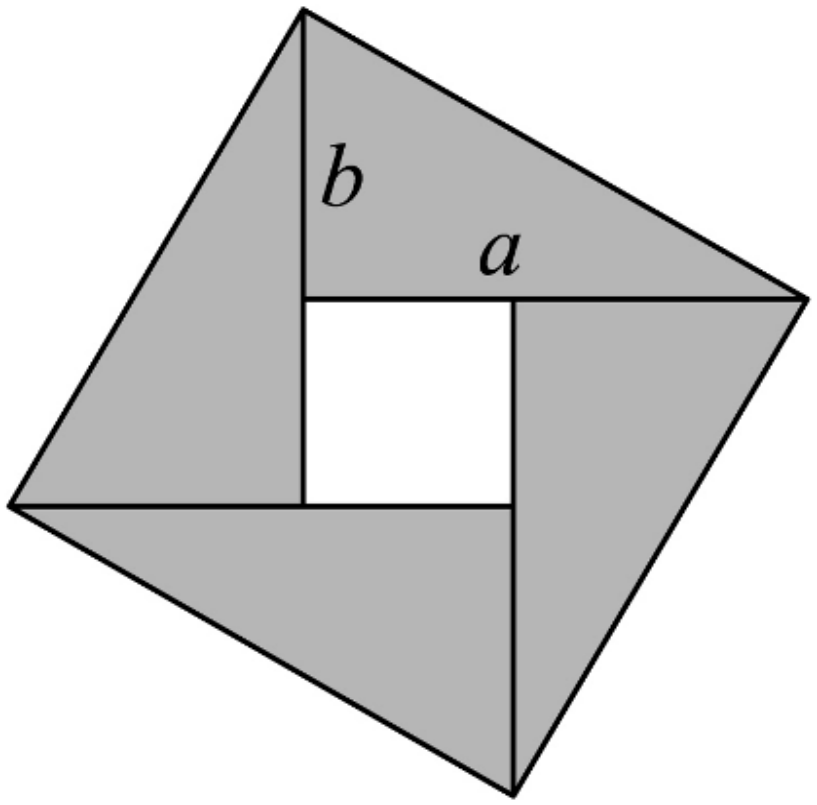
\includegraphics[width=0.20\textwidth]{figures/gao93_q16_zhaoshuang.png}
\end{center}

A. 如果 $a>b>0$，那么 $\sqrt a>\sqrt b$

B. 如果 $a>b>0$，那么 $a^2>b^2$

C. 对任意正实数 $a$ 和 $b$，有 $a^2+b^2\geqslant2ab$，当且仅当 $a=b$ 时等号成立

D. 对任意正实数 $a$ 和 $b$，有 $a^2+b^2\geqslant2ab$，当且仅当 $a=b$ 时等号成立% 原卷 C、D 两选项文字相同，照录

\ifanswer
\solbegin
\step{通过观察，可以发现这个图中的四个直角三角形是全等的，}
\step{设直角三角形的长直角边为 $a$，短直角边为 $b$，}
\step{如图，整个大正方形的面积大于等于这 $4$ 个直角三角形的面积和，}
\step{即 $a^2+b^2\geqslant4\times\left(\dfrac12ab\right)$，即 $a^2+b^2\geqslant2ab$，}
\step{当 $a=b$ 时，中间空白的正方形消失，即整个大正方形与 $4$ 个直角三角形重合；}
\step{其他选项通过该图无法证明. 故选 $C$.}
\solend
\fi

\end{enumerate}

\bigsec{三、解答题}

\begin{enumerate}
\setcounter{enumi}{16}

\item 已知 $x,y\in R$，比较 $x^2+y^2$ 与 $2(2x-y)-5$ 的大小.

\ansspace*[7]

\ifanswer
\solbegin
\step{因为 $x^2+y^2-2(2x-y)+5=(x-2)^2+(y+1)^2\geqslant0$，}
\step{所以 $x^2+y^2\geqslant2(2x-y)-5$.}
\solend
\fi

\item 设 $k\in\R$，求关于 $x$ 与 $y$ 的二元一次方程组 $\begin{cases}y=x+1\\ y=kx+3\end{cases}$ 的解集.

\ansspace*[9]

\ifanswer
\solbegin
\step{因为 $\begin{cases}y=x+1\\ y=kx+3\end{cases}$，两式相减，得到 $(k-1)x=-2$，}
\step{当 $k\neq1$ 时，$x=-\dfrac{2}{k-1}$，代入方程组中的第一式，得到 $y=\dfrac{k-3}{k-1}$，}
\step{此时，原方程组的解集为 $\left\{\left(-\dfrac{2}{k-1},\dfrac{k-3}{k-1}\right)\right\}$，}
\step{当 $k=1$ 时，方程 $(k-1)x=-2$ 无解，从而原方程组无解，其解集为空集.}
\step{综上，当 $k\neq1$ 时，解集为 $\left\{\left(-\dfrac{2}{k-1},\dfrac{k-3}{k-1}\right)\right\}$，}
\step{当 $k=1$ 时，解集为空集.}
\solend
\fi

\item 解下列不等式与方程组.

（1）解含绝对值的不等式：$\lvert x+1\rvert\geqslant3x$；

（2）求解不等式组 $\begin{cases}x^2-4x+3\geqslant0\\ \dfrac{x+3}{2x-1}\geqslant2\end{cases}$.

\ansspace*[10]

\ifanswer
\solbegin
\stepm{（1）}{当 $x\leqslant0$ 时，不等式显然成立，}
\step{当 $x>0$ 时，则 $(x+1)^2\geqslant9x^2$，得 $8x^2-2x-1\leqslant0$，}
\step{得 $(2x-1)(4x+1)\leqslant0$，解得 $-\dfrac14\leqslant x\leqslant\dfrac12$，由于 $x>0$，得 $0<x\leqslant\dfrac12$，}
\step{综上，不等式解集为 $\left\{x\left|x\leqslant\dfrac12\right.\right\}$.}
\stepm{（2）}{由 $x^2-4x+3\geqslant0$ 得 $(x-1)(x-3)\geqslant0$，所以 $x\leqslant1$ 或 $x\geqslant3$；}
\step{由 $\dfrac{x+3}{2x-1}\geqslant2$，得 $\dfrac{x+3}{2x-1}-2=\dfrac{-3x+5}{2x-1}\geqslant0$，即 $\dfrac{3x-5}{2x-1}\leqslant0$，}
\step{所以 $\begin{cases}(3x-5)(2x-1)\leqslant0\\ 2x-1\neq0\end{cases}$，解得 $\dfrac12<x\leqslant\dfrac53$，}
\step{所以不等式组的解集是 $\left\{x\left|\dfrac12<x\leqslant1\right.\right\}$.}
\solend
\fi

\item 已知关于 $x$ 的不等式 $2kx^2+kx-1<0$.

（1）若不等式的解集为 $\left(-\dfrac32,1\right)$，求实数 $k$ 的值；

（2）若不等式的解集为 $R$，求实数 $k$ 的取值范围.

\ansspace*[11]

\ifanswer
\solbegin
\stepm{（1）}{关于 $x$ 的不等式 $2kx^2+kx-1<0$ 的解集为 $\left(-\dfrac32,1\right)$，}
\step{所以 $-\dfrac32$ 和 $1$ 是方程 $2kx^2+kx-1=0$ 的两个实数根，}
\step{代入 $x=1$ 得 $2k+k-1=0$，解得 $k=\dfrac13$；}
\stepm{（2）}{若不等式 $2kx^2+kx-1<0$ 的解集为 $R$，}
\step{则 $k=0$ 时，不等式为 $-1<0$，满足题意；}
\step{$k\neq0$ 时，应满足 $\begin{cases}k<0\\ \Delta=k^2+8k<0\end{cases}$，解得 $-8<k<0$；}
\step{综上，实数 $k$ 的取值范围是 $-8<k\leqslant0$.}
\solend
\fi

\item 国家为了加强对烟酒生产的宏观管理，实行征收附加税政策，现知某种酒每瓶 $70$ 元，不征收附加税的时候，每年大约产销 $100$ 万瓶，若政府征收附加税，每销售 $100$ 元要征税 $R$ 元（叫做税率 $R\%$），则每年的销售将减少 $10R$ 万瓶.

（1）求出每年商店经营烟酒被征收的附加税税金 $S$（单位：万元）；

（2）若附加税税金 $S$ 不少于 $112$ 万元，且不大于 $168$ 万元，求 $R$ 的取值范围.

\ansspace*[12]

\ifanswer
\solbegin
\stepm{（1）}{由题意得 $S=70\times(100-10R)\times R\%(0\leqslant R\leqslant10)$（单位：万元）.}
\stepm{（2）}{由题意 $\begin{cases}70\times(100-10R)\times R\%\geqslant112\\ 70\times(100-10R)\times R\%\leqslant168\end{cases}$，解得 $2\leqslant R\leqslant4$ 或 $6\leqslant R\leqslant8$，}
\step{所以 $R$ 的取值范围是 $[2,4]\cup[6,8]$.}
\solend
\fi

\end{enumerate}

\end{document}
"
% 紧凑版：xelatex "\def\iscompact{1}% 高一93_建平世纪_10月月考.tex
%   —— 高一上数学“2026-2027 年建平世纪高一上 10 月月考”（讲评版）
% 试卷版：xelatex 高一93_建平世纪_10月月考.tex
% 答案版：xelatex "\def\isanswer{1}% 高一93_建平世纪_10月月考.tex
%   —— 高一上数学“2026-2027 年建平世纪高一上 10 月月考”（讲评版）
% 试卷版：xelatex 高一93_建平世纪_10月月考.tex
% 答案版：xelatex "\def\isanswer{1}% 高一93_建平世纪_10月月考.tex
%   —— 高一上数学“2026-2027 年建平世纪高一上 10 月月考”（讲评版）
% 试卷版：xelatex 高一93_建平世纪_10月月考.tex
% 答案版：xelatex "\def\isanswer{1}\input{高一93_建平世纪_10月月考.tex}"
% 紧凑版：xelatex "\def\iscompact{1}\input{高一93_建平世纪_10月月考.tex}"
%
% 原始材料：微信公众号“魔都数学加油站”文章，连载“27学年高一93”；
% 原文标题“27学年高一93——2026-2027年上海市建平世纪高一上10月月考”；
% 原文链接：https://mp.weixin.qq.com/s/uqySZX3I8Q-QZ2J8MqmWiA。
% 正文为 7 张 PNG 页（`原图/高一93_建平世纪_10月月考/01..07.png`），均 4762×6735，按页序读取。
%
% 篇幅与题号：原卷自第 3 题起编号（第 1、2 题不在原文内）。填空题 3—12（10 题）、
% 选择题 13—16（4 题）、解答题 17—21（5 题），共 19 题。
%
% 讲评版：第 3、4 题只印【答案】（“$\{x\mid-1<x<1\}$”“$x$ 和 $y$ 不都是有理数”），本稿只给 \ans{}；
% 其余 17 题印【解析】，其中选择题答案在解析末句“故选 $D$／$D$／$C$／$C$”。
% 第 16 题题干右侧有一幅赵爽弦图（裁自第 4 页原图、去粉色水印后转灰度）。
%
% 副标题：原卷未印副标题。本稿按内容标作“集合与常用逻辑用语、不等式”。
%
% 原卷笔误/存疑（均照录未改，正文对应处另有 % 注）：
%   ① 第 3 题答案印作 $\{x\mid-1<x<1\}$（两端开），而 $\lvert x\rvert\leqslant1$ 的解集应为
%      $[-1,1]$（两端闭）；原卷照录，未改；
%   ② 第 16 题 C、D 两个选项**文字完全相同**（皆为“对任意正实数 $a$ 和 $b$，有
%      $a^2+b^2\geqslant2ab$，当且仅当 $a=b$ 时等号成立”），原卷重复排印；答案取 $C$，
%      本稿两个选项照录。
%
% 与原卷的排版差异：
%   ① 原卷每题下直接印【答案】/【解析】，本稿按全稿惯例将答案与解析置于答案版；
%   ② 原卷未印副标题，本稿补出；填空横线统一排 \blankline[4.4em]；
%   ③ 原卷数集记号排斜体 $R$，本稿按全稿惯例改用 $\R$；
%   ④ 第 17—21 题的子问用行内“（1）（2）（3）”段，解析中的子问标号用 \stepm；
%   ⑤ 解答题按惯例加 \ansspace；选择题括号排 \mbox{（\quad）}；
%   ⑥ 第 16 题的弦图原卷排在题干右侧、文字绕排，本稿改排为选项后的居中图。
%
% 行数核对：逐题数 \step/\stepm 条数，合计 71 条（Q3：0；Q4：0；Q5：2；Q6：3；Q7：2；
% Q8：2；Q9：4；Q10：1；Q11：3；Q12：9；Q13：5；Q14：3；Q15：5；Q16：6；Q17：2；
% Q18：6；Q19：8；Q20：7；Q21：3）。第 3、4 题只印答案，不计入 \step 账。
% 原卷解析的换行按语意合并，未逐行强拆。
%
\documentclass[a4paper,11pt]{article}
\usepackage{common}

\begin{document}

\examtitlest[7]{2026--2027 年建平世纪高一上 10 月月考}{集合与常用逻辑用语、不等式}

\bigsec{一、填空题}

\begin{enumerate}
\setcounter{enumi}{2}

\item 不等式 $\lvert x\rvert\leqslant1$ 的解集是\blankline[4.4em].

\ifanswer
\ans{$\{x\mid-1<x<1\}$}% 原卷答案两端开；|x|≤1 应为 [-1,1]，照录
\fi

\item “$x$ 和 $y$ 都是有理数”的否定形式是\blankline[4.4em].

\ifanswer
\ans{$x$ 和 $y$ 不都是有理数}
\fi

\item 已知等式 $2x^2+3x+5=2ax^2+a(3x+1)+c$ 恒成立，则 $a+c=\blankline[4.4em]$.

\ifanswer
\solbegin
\step{因为 $2x^2+3x+5=2ax^2+a(3x+1)+c$ 恒成立，}
\step{即 $2x^2+3x+5=2ax^2+3ax+(a+c)$ 恒成立，所以 $\begin{cases}2=2a\\ 3=3a\\ 5=a+c\end{cases}$，所以 $a+c=5$.}
\solend
\fi

\item 已知方程 $x^2+6x+m=0(m\in\R)$ 的两个根 $x_1$、$x_2$ 满足 $\lvert x_1-x_2\rvert=4$，则 $m$ 的值是\blankline[4.4em].

\ifanswer
\solbegin
\step{方程 $x^2+6x+m=0(m\in\R)$ 的两根为 $x_1$、$x_2$，所以 $x_1+x_2=-6$，$x_1x_2=m$，}
\step{又 $\lvert x_1-x_2\rvert=4$，则 $(x_1-x_2)^2=(x_1+x_2)^2-4x_1x_2=16$，}
\step{即 $(-6)^2-4m=16$，解得 $m=5$，检验得 $\Delta=6^2-4\times1\times5=16>0$，符合题意，所以 $m=5$.}
\solend
\fi

\item 已知 $\alpha:2m-6<x<m+5$，$\beta:-3<x<5$，若 $\alpha$ 是 $\beta$ 的必要条件，则实数 $m$ 的取值范围是\blankline[4.4em].

\ifanswer
\solbegin
\step{因为 $\alpha$ 是 $\beta$ 的必要条件，所以 $\begin{cases}2m-6\leqslant-3\\ m+5\geqslant5\\ 2m-6<m+5\end{cases}\Rightarrow0\leqslant m\leqslant\dfrac32$，}
\step{所以实数 $m$ 的取值范围是 $\left[0,\dfrac32\right]$.}
\solend
\fi

\item 已知 $-2\leqslant a\leqslant3$，$2\leqslant b\leqslant\dfrac72$，则 $a-2b$ 的取值范围为\blankline[4.4em].

\ifanswer
\solbegin
\step{因为 $-2\leqslant a\leqslant3$，$2\leqslant b\leqslant\dfrac72$，所以 $-7\leqslant-2b\leqslant-4$，所以 $-9\leqslant a-2b\leqslant-1$，}
\step{故 $a-2b$ 的取值范围为 $[-9,-1]$.}
\solend
\fi

\item 已知 $\lvert x+3\rvert+\lvert5-x\rvert>10$，则实数 $x$ 的取值范围为\blankline[4.4em].

\ifanswer
\solbegin
\step{当 $x<-3$ 时，则 $-x-3+5-x>10$，解得 $x<-4$，}
\step{当 $-3\leqslant x\leqslant5$ 时，则 $x+3+5-x=8<10$，原不等式不成立，}
\step{当 $x>5$ 时，则 $x+3+x-5>10$，解得 $x>6$，}
\step{综上所述，实数 $x$ 的取值范围为 $(-\infty,-4)\cup(6,+\infty)$.}
\solend
\fi

\item 已知集合 $A=\{(x,y)\mid y=x+1\}$，$B=\{(x,y)\mid y=-x+3\}$，则 $A\cap B=\blankline[4.4em]$.

\ifanswer
\solbegin
\step{联立 $\begin{cases}y=x+1\\ y=-x+3\end{cases}$，解得 $x=1$，$y=2$，故 $A\cap B=\{(1,2)\}$.}
\solend
\fi

\item 若关于 $x$ 的不等式组 $\begin{cases}\dfrac{x-1}{x-3}<0\\ x>a\end{cases}$ 的解集为空集，则实数 $a$ 的取值范围为\blankline[4.4em].

\ifanswer
\solbegin
\step{$\dfrac{x-1}{x-3}<0$ 等价于 $(x-1)(x-3)<0$，得 $1<x<3$，}
\step{因为 $\begin{cases}\dfrac{x-1}{x-3}<0\\ x>a\end{cases}$ 的解集为空集，}
\step{所以 $a\geqslant3$，故实数 $a$ 的取值范围为 $[3,+\infty)$.}
\solend
\fi

\item 已知由自然数组成的 $n-1$ 个元素的集合 $A=\{1,2,3,4,\cdots,n-1\}(n>1)$，非空集合 $B\subseteq A$，且对任意的 $a\in B$，都有 $n-a\in B$. 当 $n=9$ 时，则所有满足条件的集合 $B$ 的元素的和为\blankline[4.4em].

\ifanswer
\solbegin
\step{当 $n=9$ 时，$A=\{1,2,3,4,5,6,7,8\}$，}
\step{当 $B$ 中有两个元素时，集合 $B$ 可以为 $\{1,8\},\{2,7\},\{3,6\},\{4,5\}$，}
\step{元素总和为 $4\times9=36$；}
\step{当 $B$ 中有四个元素时，集合 $B$ 可以为 $\{1,8\},\{2,7\},\{3,6\},\{4,5\}$ 中任取两个的并集，}
\step{集合 $B$ 共有 $6$ 种情况，元素总和为 $6\times2\times9=108$；}
\step{当 $B$ 中有六个元素时，集合 $B$ 可以为 $\{1,8\},\{2,7\},\{3,6\},\{4,5\}$ 中任取三个的并集，}
\step{集合 $B$ 共有 $4$ 种情况，元素总和为 $4\times3\times9=12\times9=108$；}
\step{当 $B$ 中有八个元素时，$B=\{1,2,3,4,5,6,7,8\}$，元素之和为 $4\times9=36$，}
\step{所以所有满足条件的集合 $B$ 的元素总和为 $36+108+108+36=288$.}
\solend
\fi

\end{enumerate}

\bigsec{二、选择题}

\begin{enumerate}
\setcounter{enumi}{12}

\item 下列说法正确的是\mbox{（\quad）}

\keepwithprev
A. 若 $a>b$，则 $\dfrac1a<\dfrac1b$\qquad B. 若 $a>b,c>d$，则 $ac>bd$

C. 若 $a>b$，则 $ac^2>bc^2$\qquad D. 若 $ac^2>bc^2$，则 $a>b$

\ifanswer
\solbegin
\step{A：令 $a=2,b=-1$，此时 $\dfrac12>-1$，故 A 错误；}
\step{B：令 $a=2,b=-1,c=0,d=-2$，此时 $ac=0<bd=2$，故 B 错误；}
\step{C：由 $a>b$，当 $c=0$ 时，$ac^2=bc^2$，故 C 错误；}
\step{D：由 $ac^2>bc^2$，则 $c^2>0$，所以 $a>b$，故 D 正确.}
\step{故选 $D$.}
\solend
\fi

\item 不等式 $\dfrac{x-3}{x-1}\leqslant2$ 的解集是\mbox{（\quad）}

\keepwithprev
A. $(-\infty,1]$\qquad B. $[1,+\infty)$

C. $(-\infty,-1]\cup[1,+\infty)$\qquad D. $(-\infty,-1]\cup(1,+\infty)$

\ifanswer
\solbegin
\step{不等式 $\dfrac{x-3}{x-1}\leqslant2$ 可化为 $\dfrac{x-3}{x-1}-2\leqslant0$，即 $\dfrac{x-3-2(x-1)}{x-1}\leqslant0$，}
\step{化简得 $\dfrac{x+1}{x-1}\geqslant0$，等价于 $\begin{cases}(x+1)(x-1)\geqslant0\\ x\neq1\end{cases}$，解得 $x\leqslant-1$ 或 $x>1$，}
\step{所以不等式的解集为 $(-\infty,-1]\cup(1,+\infty)$. 故选 $D$.}
\solend
\fi

\item 已知集合 $M$ 和集合 $N$，那么 $M\cap N=N$ 的充要条件是\mbox{（\quad）}

\keepwithprev
A. $M\subseteq N$\qquad B. $N\subset M$\qquad C. $M\supseteq N$\qquad D. $M=N$

\ifanswer
\solbegin
\step{若 $M\subseteq N$，即集合 $M$ 是集合 $N$ 的子集，则 $M\cap N=M$，故 $A$ 错误；}
\step{若 $M=N$，则不能得到 $N\subset M$，故 $B$ 错误；}
\step{若 $M\cap N=N$，则 $M\supseteq N$，故 $C$ 正确；}
\step{当 $N$ 是 $M$ 真子集时，不能得到 $M=N$，故 $D$ 错误.}
\step{故选 $C$.}
\solend
\fi

\item 三国时期赵爽在《勾股方圆图注》中对勾股定理的证明可用现代数学表述为如图所示，我们教材中利用该图作为“（\quad）”的几何解释.

\begin{center}
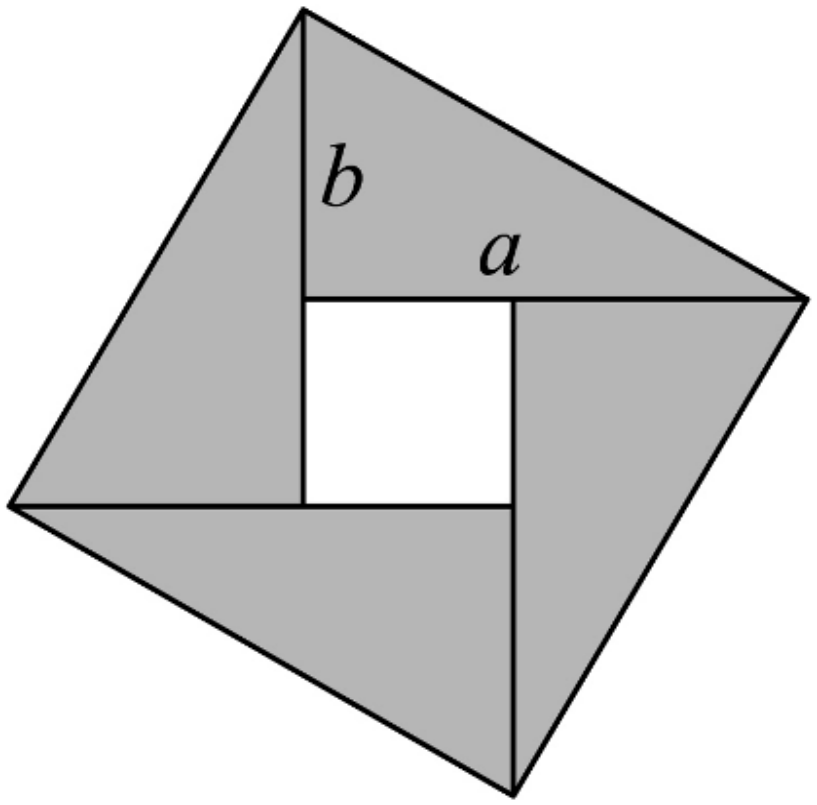
\includegraphics[width=0.20\textwidth]{figures/gao93_q16_zhaoshuang.png}
\end{center}

A. 如果 $a>b>0$，那么 $\sqrt a>\sqrt b$

B. 如果 $a>b>0$，那么 $a^2>b^2$

C. 对任意正实数 $a$ 和 $b$，有 $a^2+b^2\geqslant2ab$，当且仅当 $a=b$ 时等号成立

D. 对任意正实数 $a$ 和 $b$，有 $a^2+b^2\geqslant2ab$，当且仅当 $a=b$ 时等号成立% 原卷 C、D 两选项文字相同，照录

\ifanswer
\solbegin
\step{通过观察，可以发现这个图中的四个直角三角形是全等的，}
\step{设直角三角形的长直角边为 $a$，短直角边为 $b$，}
\step{如图，整个大正方形的面积大于等于这 $4$ 个直角三角形的面积和，}
\step{即 $a^2+b^2\geqslant4\times\left(\dfrac12ab\right)$，即 $a^2+b^2\geqslant2ab$，}
\step{当 $a=b$ 时，中间空白的正方形消失，即整个大正方形与 $4$ 个直角三角形重合；}
\step{其他选项通过该图无法证明. 故选 $C$.}
\solend
\fi

\end{enumerate}

\bigsec{三、解答题}

\begin{enumerate}
\setcounter{enumi}{16}

\item 已知 $x,y\in R$，比较 $x^2+y^2$ 与 $2(2x-y)-5$ 的大小.

\ansspace*[7]

\ifanswer
\solbegin
\step{因为 $x^2+y^2-2(2x-y)+5=(x-2)^2+(y+1)^2\geqslant0$，}
\step{所以 $x^2+y^2\geqslant2(2x-y)-5$.}
\solend
\fi

\item 设 $k\in\R$，求关于 $x$ 与 $y$ 的二元一次方程组 $\begin{cases}y=x+1\\ y=kx+3\end{cases}$ 的解集.

\ansspace*[9]

\ifanswer
\solbegin
\step{因为 $\begin{cases}y=x+1\\ y=kx+3\end{cases}$，两式相减，得到 $(k-1)x=-2$，}
\step{当 $k\neq1$ 时，$x=-\dfrac{2}{k-1}$，代入方程组中的第一式，得到 $y=\dfrac{k-3}{k-1}$，}
\step{此时，原方程组的解集为 $\left\{\left(-\dfrac{2}{k-1},\dfrac{k-3}{k-1}\right)\right\}$，}
\step{当 $k=1$ 时，方程 $(k-1)x=-2$ 无解，从而原方程组无解，其解集为空集.}
\step{综上，当 $k\neq1$ 时，解集为 $\left\{\left(-\dfrac{2}{k-1},\dfrac{k-3}{k-1}\right)\right\}$，}
\step{当 $k=1$ 时，解集为空集.}
\solend
\fi

\item 解下列不等式与方程组.

（1）解含绝对值的不等式：$\lvert x+1\rvert\geqslant3x$；

（2）求解不等式组 $\begin{cases}x^2-4x+3\geqslant0\\ \dfrac{x+3}{2x-1}\geqslant2\end{cases}$.

\ansspace*[10]

\ifanswer
\solbegin
\stepm{（1）}{当 $x\leqslant0$ 时，不等式显然成立，}
\step{当 $x>0$ 时，则 $(x+1)^2\geqslant9x^2$，得 $8x^2-2x-1\leqslant0$，}
\step{得 $(2x-1)(4x+1)\leqslant0$，解得 $-\dfrac14\leqslant x\leqslant\dfrac12$，由于 $x>0$，得 $0<x\leqslant\dfrac12$，}
\step{综上，不等式解集为 $\left\{x\left|x\leqslant\dfrac12\right.\right\}$.}
\stepm{（2）}{由 $x^2-4x+3\geqslant0$ 得 $(x-1)(x-3)\geqslant0$，所以 $x\leqslant1$ 或 $x\geqslant3$；}
\step{由 $\dfrac{x+3}{2x-1}\geqslant2$，得 $\dfrac{x+3}{2x-1}-2=\dfrac{-3x+5}{2x-1}\geqslant0$，即 $\dfrac{3x-5}{2x-1}\leqslant0$，}
\step{所以 $\begin{cases}(3x-5)(2x-1)\leqslant0\\ 2x-1\neq0\end{cases}$，解得 $\dfrac12<x\leqslant\dfrac53$，}
\step{所以不等式组的解集是 $\left\{x\left|\dfrac12<x\leqslant1\right.\right\}$.}
\solend
\fi

\item 已知关于 $x$ 的不等式 $2kx^2+kx-1<0$.

（1）若不等式的解集为 $\left(-\dfrac32,1\right)$，求实数 $k$ 的值；

（2）若不等式的解集为 $R$，求实数 $k$ 的取值范围.

\ansspace*[11]

\ifanswer
\solbegin
\stepm{（1）}{关于 $x$ 的不等式 $2kx^2+kx-1<0$ 的解集为 $\left(-\dfrac32,1\right)$，}
\step{所以 $-\dfrac32$ 和 $1$ 是方程 $2kx^2+kx-1=0$ 的两个实数根，}
\step{代入 $x=1$ 得 $2k+k-1=0$，解得 $k=\dfrac13$；}
\stepm{（2）}{若不等式 $2kx^2+kx-1<0$ 的解集为 $R$，}
\step{则 $k=0$ 时，不等式为 $-1<0$，满足题意；}
\step{$k\neq0$ 时，应满足 $\begin{cases}k<0\\ \Delta=k^2+8k<0\end{cases}$，解得 $-8<k<0$；}
\step{综上，实数 $k$ 的取值范围是 $-8<k\leqslant0$.}
\solend
\fi

\item 国家为了加强对烟酒生产的宏观管理，实行征收附加税政策，现知某种酒每瓶 $70$ 元，不征收附加税的时候，每年大约产销 $100$ 万瓶，若政府征收附加税，每销售 $100$ 元要征税 $R$ 元（叫做税率 $R\%$），则每年的销售将减少 $10R$ 万瓶.

（1）求出每年商店经营烟酒被征收的附加税税金 $S$（单位：万元）；

（2）若附加税税金 $S$ 不少于 $112$ 万元，且不大于 $168$ 万元，求 $R$ 的取值范围.

\ansspace*[12]

\ifanswer
\solbegin
\stepm{（1）}{由题意得 $S=70\times(100-10R)\times R\%(0\leqslant R\leqslant10)$（单位：万元）.}
\stepm{（2）}{由题意 $\begin{cases}70\times(100-10R)\times R\%\geqslant112\\ 70\times(100-10R)\times R\%\leqslant168\end{cases}$，解得 $2\leqslant R\leqslant4$ 或 $6\leqslant R\leqslant8$，}
\step{所以 $R$ 的取值范围是 $[2,4]\cup[6,8]$.}
\solend
\fi

\end{enumerate}

\end{document}
"
% 紧凑版：xelatex "\def\iscompact{1}% 高一93_建平世纪_10月月考.tex
%   —— 高一上数学“2026-2027 年建平世纪高一上 10 月月考”（讲评版）
% 试卷版：xelatex 高一93_建平世纪_10月月考.tex
% 答案版：xelatex "\def\isanswer{1}\input{高一93_建平世纪_10月月考.tex}"
% 紧凑版：xelatex "\def\iscompact{1}\input{高一93_建平世纪_10月月考.tex}"
%
% 原始材料：微信公众号“魔都数学加油站”文章，连载“27学年高一93”；
% 原文标题“27学年高一93——2026-2027年上海市建平世纪高一上10月月考”；
% 原文链接：https://mp.weixin.qq.com/s/uqySZX3I8Q-QZ2J8MqmWiA。
% 正文为 7 张 PNG 页（`原图/高一93_建平世纪_10月月考/01..07.png`），均 4762×6735，按页序读取。
%
% 篇幅与题号：原卷自第 3 题起编号（第 1、2 题不在原文内）。填空题 3—12（10 题）、
% 选择题 13—16（4 题）、解答题 17—21（5 题），共 19 题。
%
% 讲评版：第 3、4 题只印【答案】（“$\{x\mid-1<x<1\}$”“$x$ 和 $y$ 不都是有理数”），本稿只给 \ans{}；
% 其余 17 题印【解析】，其中选择题答案在解析末句“故选 $D$／$D$／$C$／$C$”。
% 第 16 题题干右侧有一幅赵爽弦图（裁自第 4 页原图、去粉色水印后转灰度）。
%
% 副标题：原卷未印副标题。本稿按内容标作“集合与常用逻辑用语、不等式”。
%
% 原卷笔误/存疑（均照录未改，正文对应处另有 % 注）：
%   ① 第 3 题答案印作 $\{x\mid-1<x<1\}$（两端开），而 $\lvert x\rvert\leqslant1$ 的解集应为
%      $[-1,1]$（两端闭）；原卷照录，未改；
%   ② 第 16 题 C、D 两个选项**文字完全相同**（皆为“对任意正实数 $a$ 和 $b$，有
%      $a^2+b^2\geqslant2ab$，当且仅当 $a=b$ 时等号成立”），原卷重复排印；答案取 $C$，
%      本稿两个选项照录。
%
% 与原卷的排版差异：
%   ① 原卷每题下直接印【答案】/【解析】，本稿按全稿惯例将答案与解析置于答案版；
%   ② 原卷未印副标题，本稿补出；填空横线统一排 \blankline[4.4em]；
%   ③ 原卷数集记号排斜体 $R$，本稿按全稿惯例改用 $\R$；
%   ④ 第 17—21 题的子问用行内“（1）（2）（3）”段，解析中的子问标号用 \stepm；
%   ⑤ 解答题按惯例加 \ansspace；选择题括号排 \mbox{（\quad）}；
%   ⑥ 第 16 题的弦图原卷排在题干右侧、文字绕排，本稿改排为选项后的居中图。
%
% 行数核对：逐题数 \step/\stepm 条数，合计 71 条（Q3：0；Q4：0；Q5：2；Q6：3；Q7：2；
% Q8：2；Q9：4；Q10：1；Q11：3；Q12：9；Q13：5；Q14：3；Q15：5；Q16：6；Q17：2；
% Q18：6；Q19：8；Q20：7；Q21：3）。第 3、4 题只印答案，不计入 \step 账。
% 原卷解析的换行按语意合并，未逐行强拆。
%
\documentclass[a4paper,11pt]{article}
\usepackage{common}

\begin{document}

\examtitlest[7]{2026--2027 年建平世纪高一上 10 月月考}{集合与常用逻辑用语、不等式}

\bigsec{一、填空题}

\begin{enumerate}
\setcounter{enumi}{2}

\item 不等式 $\lvert x\rvert\leqslant1$ 的解集是\blankline[4.4em].

\ifanswer
\ans{$\{x\mid-1<x<1\}$}% 原卷答案两端开；|x|≤1 应为 [-1,1]，照录
\fi

\item “$x$ 和 $y$ 都是有理数”的否定形式是\blankline[4.4em].

\ifanswer
\ans{$x$ 和 $y$ 不都是有理数}
\fi

\item 已知等式 $2x^2+3x+5=2ax^2+a(3x+1)+c$ 恒成立，则 $a+c=\blankline[4.4em]$.

\ifanswer
\solbegin
\step{因为 $2x^2+3x+5=2ax^2+a(3x+1)+c$ 恒成立，}
\step{即 $2x^2+3x+5=2ax^2+3ax+(a+c)$ 恒成立，所以 $\begin{cases}2=2a\\ 3=3a\\ 5=a+c\end{cases}$，所以 $a+c=5$.}
\solend
\fi

\item 已知方程 $x^2+6x+m=0(m\in\R)$ 的两个根 $x_1$、$x_2$ 满足 $\lvert x_1-x_2\rvert=4$，则 $m$ 的值是\blankline[4.4em].

\ifanswer
\solbegin
\step{方程 $x^2+6x+m=0(m\in\R)$ 的两根为 $x_1$、$x_2$，所以 $x_1+x_2=-6$，$x_1x_2=m$，}
\step{又 $\lvert x_1-x_2\rvert=4$，则 $(x_1-x_2)^2=(x_1+x_2)^2-4x_1x_2=16$，}
\step{即 $(-6)^2-4m=16$，解得 $m=5$，检验得 $\Delta=6^2-4\times1\times5=16>0$，符合题意，所以 $m=5$.}
\solend
\fi

\item 已知 $\alpha:2m-6<x<m+5$，$\beta:-3<x<5$，若 $\alpha$ 是 $\beta$ 的必要条件，则实数 $m$ 的取值范围是\blankline[4.4em].

\ifanswer
\solbegin
\step{因为 $\alpha$ 是 $\beta$ 的必要条件，所以 $\begin{cases}2m-6\leqslant-3\\ m+5\geqslant5\\ 2m-6<m+5\end{cases}\Rightarrow0\leqslant m\leqslant\dfrac32$，}
\step{所以实数 $m$ 的取值范围是 $\left[0,\dfrac32\right]$.}
\solend
\fi

\item 已知 $-2\leqslant a\leqslant3$，$2\leqslant b\leqslant\dfrac72$，则 $a-2b$ 的取值范围为\blankline[4.4em].

\ifanswer
\solbegin
\step{因为 $-2\leqslant a\leqslant3$，$2\leqslant b\leqslant\dfrac72$，所以 $-7\leqslant-2b\leqslant-4$，所以 $-9\leqslant a-2b\leqslant-1$，}
\step{故 $a-2b$ 的取值范围为 $[-9,-1]$.}
\solend
\fi

\item 已知 $\lvert x+3\rvert+\lvert5-x\rvert>10$，则实数 $x$ 的取值范围为\blankline[4.4em].

\ifanswer
\solbegin
\step{当 $x<-3$ 时，则 $-x-3+5-x>10$，解得 $x<-4$，}
\step{当 $-3\leqslant x\leqslant5$ 时，则 $x+3+5-x=8<10$，原不等式不成立，}
\step{当 $x>5$ 时，则 $x+3+x-5>10$，解得 $x>6$，}
\step{综上所述，实数 $x$ 的取值范围为 $(-\infty,-4)\cup(6,+\infty)$.}
\solend
\fi

\item 已知集合 $A=\{(x,y)\mid y=x+1\}$，$B=\{(x,y)\mid y=-x+3\}$，则 $A\cap B=\blankline[4.4em]$.

\ifanswer
\solbegin
\step{联立 $\begin{cases}y=x+1\\ y=-x+3\end{cases}$，解得 $x=1$，$y=2$，故 $A\cap B=\{(1,2)\}$.}
\solend
\fi

\item 若关于 $x$ 的不等式组 $\begin{cases}\dfrac{x-1}{x-3}<0\\ x>a\end{cases}$ 的解集为空集，则实数 $a$ 的取值范围为\blankline[4.4em].

\ifanswer
\solbegin
\step{$\dfrac{x-1}{x-3}<0$ 等价于 $(x-1)(x-3)<0$，得 $1<x<3$，}
\step{因为 $\begin{cases}\dfrac{x-1}{x-3}<0\\ x>a\end{cases}$ 的解集为空集，}
\step{所以 $a\geqslant3$，故实数 $a$ 的取值范围为 $[3,+\infty)$.}
\solend
\fi

\item 已知由自然数组成的 $n-1$ 个元素的集合 $A=\{1,2,3,4,\cdots,n-1\}(n>1)$，非空集合 $B\subseteq A$，且对任意的 $a\in B$，都有 $n-a\in B$. 当 $n=9$ 时，则所有满足条件的集合 $B$ 的元素的和为\blankline[4.4em].

\ifanswer
\solbegin
\step{当 $n=9$ 时，$A=\{1,2,3,4,5,6,7,8\}$，}
\step{当 $B$ 中有两个元素时，集合 $B$ 可以为 $\{1,8\},\{2,7\},\{3,6\},\{4,5\}$，}
\step{元素总和为 $4\times9=36$；}
\step{当 $B$ 中有四个元素时，集合 $B$ 可以为 $\{1,8\},\{2,7\},\{3,6\},\{4,5\}$ 中任取两个的并集，}
\step{集合 $B$ 共有 $6$ 种情况，元素总和为 $6\times2\times9=108$；}
\step{当 $B$ 中有六个元素时，集合 $B$ 可以为 $\{1,8\},\{2,7\},\{3,6\},\{4,5\}$ 中任取三个的并集，}
\step{集合 $B$ 共有 $4$ 种情况，元素总和为 $4\times3\times9=12\times9=108$；}
\step{当 $B$ 中有八个元素时，$B=\{1,2,3,4,5,6,7,8\}$，元素之和为 $4\times9=36$，}
\step{所以所有满足条件的集合 $B$ 的元素总和为 $36+108+108+36=288$.}
\solend
\fi

\end{enumerate}

\bigsec{二、选择题}

\begin{enumerate}
\setcounter{enumi}{12}

\item 下列说法正确的是\mbox{（\quad）}

\keepwithprev
A. 若 $a>b$，则 $\dfrac1a<\dfrac1b$\qquad B. 若 $a>b,c>d$，则 $ac>bd$

C. 若 $a>b$，则 $ac^2>bc^2$\qquad D. 若 $ac^2>bc^2$，则 $a>b$

\ifanswer
\solbegin
\step{A：令 $a=2,b=-1$，此时 $\dfrac12>-1$，故 A 错误；}
\step{B：令 $a=2,b=-1,c=0,d=-2$，此时 $ac=0<bd=2$，故 B 错误；}
\step{C：由 $a>b$，当 $c=0$ 时，$ac^2=bc^2$，故 C 错误；}
\step{D：由 $ac^2>bc^2$，则 $c^2>0$，所以 $a>b$，故 D 正确.}
\step{故选 $D$.}
\solend
\fi

\item 不等式 $\dfrac{x-3}{x-1}\leqslant2$ 的解集是\mbox{（\quad）}

\keepwithprev
A. $(-\infty,1]$\qquad B. $[1,+\infty)$

C. $(-\infty,-1]\cup[1,+\infty)$\qquad D. $(-\infty,-1]\cup(1,+\infty)$

\ifanswer
\solbegin
\step{不等式 $\dfrac{x-3}{x-1}\leqslant2$ 可化为 $\dfrac{x-3}{x-1}-2\leqslant0$，即 $\dfrac{x-3-2(x-1)}{x-1}\leqslant0$，}
\step{化简得 $\dfrac{x+1}{x-1}\geqslant0$，等价于 $\begin{cases}(x+1)(x-1)\geqslant0\\ x\neq1\end{cases}$，解得 $x\leqslant-1$ 或 $x>1$，}
\step{所以不等式的解集为 $(-\infty,-1]\cup(1,+\infty)$. 故选 $D$.}
\solend
\fi

\item 已知集合 $M$ 和集合 $N$，那么 $M\cap N=N$ 的充要条件是\mbox{（\quad）}

\keepwithprev
A. $M\subseteq N$\qquad B. $N\subset M$\qquad C. $M\supseteq N$\qquad D. $M=N$

\ifanswer
\solbegin
\step{若 $M\subseteq N$，即集合 $M$ 是集合 $N$ 的子集，则 $M\cap N=M$，故 $A$ 错误；}
\step{若 $M=N$，则不能得到 $N\subset M$，故 $B$ 错误；}
\step{若 $M\cap N=N$，则 $M\supseteq N$，故 $C$ 正确；}
\step{当 $N$ 是 $M$ 真子集时，不能得到 $M=N$，故 $D$ 错误.}
\step{故选 $C$.}
\solend
\fi

\item 三国时期赵爽在《勾股方圆图注》中对勾股定理的证明可用现代数学表述为如图所示，我们教材中利用该图作为“（\quad）”的几何解释.

\begin{center}
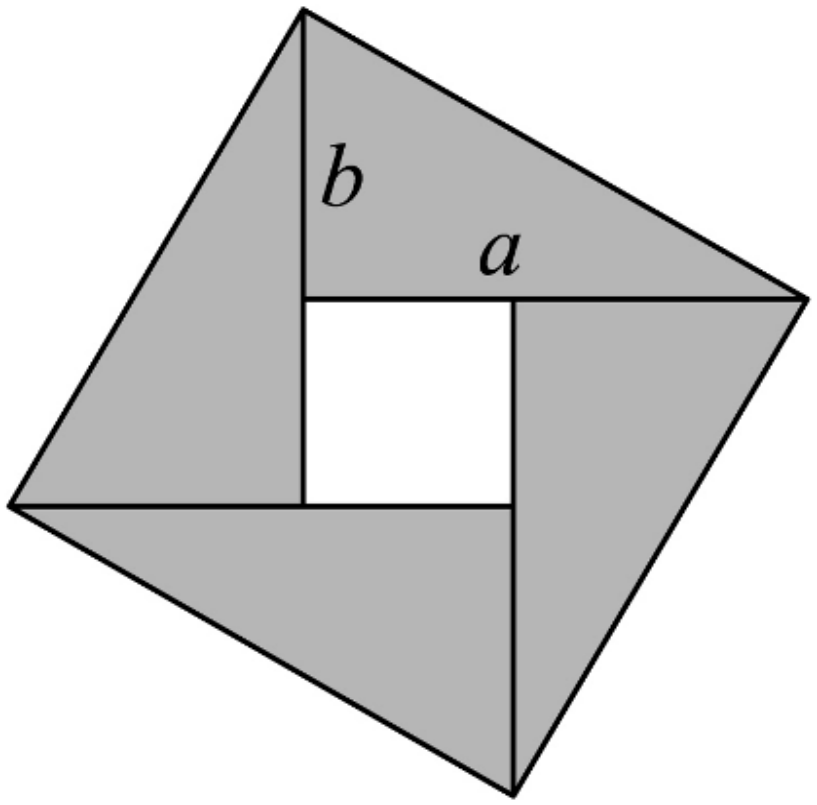
\includegraphics[width=0.20\textwidth]{figures/gao93_q16_zhaoshuang.png}
\end{center}

A. 如果 $a>b>0$，那么 $\sqrt a>\sqrt b$

B. 如果 $a>b>0$，那么 $a^2>b^2$

C. 对任意正实数 $a$ 和 $b$，有 $a^2+b^2\geqslant2ab$，当且仅当 $a=b$ 时等号成立

D. 对任意正实数 $a$ 和 $b$，有 $a^2+b^2\geqslant2ab$，当且仅当 $a=b$ 时等号成立% 原卷 C、D 两选项文字相同，照录

\ifanswer
\solbegin
\step{通过观察，可以发现这个图中的四个直角三角形是全等的，}
\step{设直角三角形的长直角边为 $a$，短直角边为 $b$，}
\step{如图，整个大正方形的面积大于等于这 $4$ 个直角三角形的面积和，}
\step{即 $a^2+b^2\geqslant4\times\left(\dfrac12ab\right)$，即 $a^2+b^2\geqslant2ab$，}
\step{当 $a=b$ 时，中间空白的正方形消失，即整个大正方形与 $4$ 个直角三角形重合；}
\step{其他选项通过该图无法证明. 故选 $C$.}
\solend
\fi

\end{enumerate}

\bigsec{三、解答题}

\begin{enumerate}
\setcounter{enumi}{16}

\item 已知 $x,y\in R$，比较 $x^2+y^2$ 与 $2(2x-y)-5$ 的大小.

\ansspace*[7]

\ifanswer
\solbegin
\step{因为 $x^2+y^2-2(2x-y)+5=(x-2)^2+(y+1)^2\geqslant0$，}
\step{所以 $x^2+y^2\geqslant2(2x-y)-5$.}
\solend
\fi

\item 设 $k\in\R$，求关于 $x$ 与 $y$ 的二元一次方程组 $\begin{cases}y=x+1\\ y=kx+3\end{cases}$ 的解集.

\ansspace*[9]

\ifanswer
\solbegin
\step{因为 $\begin{cases}y=x+1\\ y=kx+3\end{cases}$，两式相减，得到 $(k-1)x=-2$，}
\step{当 $k\neq1$ 时，$x=-\dfrac{2}{k-1}$，代入方程组中的第一式，得到 $y=\dfrac{k-3}{k-1}$，}
\step{此时，原方程组的解集为 $\left\{\left(-\dfrac{2}{k-1},\dfrac{k-3}{k-1}\right)\right\}$，}
\step{当 $k=1$ 时，方程 $(k-1)x=-2$ 无解，从而原方程组无解，其解集为空集.}
\step{综上，当 $k\neq1$ 时，解集为 $\left\{\left(-\dfrac{2}{k-1},\dfrac{k-3}{k-1}\right)\right\}$，}
\step{当 $k=1$ 时，解集为空集.}
\solend
\fi

\item 解下列不等式与方程组.

（1）解含绝对值的不等式：$\lvert x+1\rvert\geqslant3x$；

（2）求解不等式组 $\begin{cases}x^2-4x+3\geqslant0\\ \dfrac{x+3}{2x-1}\geqslant2\end{cases}$.

\ansspace*[10]

\ifanswer
\solbegin
\stepm{（1）}{当 $x\leqslant0$ 时，不等式显然成立，}
\step{当 $x>0$ 时，则 $(x+1)^2\geqslant9x^2$，得 $8x^2-2x-1\leqslant0$，}
\step{得 $(2x-1)(4x+1)\leqslant0$，解得 $-\dfrac14\leqslant x\leqslant\dfrac12$，由于 $x>0$，得 $0<x\leqslant\dfrac12$，}
\step{综上，不等式解集为 $\left\{x\left|x\leqslant\dfrac12\right.\right\}$.}
\stepm{（2）}{由 $x^2-4x+3\geqslant0$ 得 $(x-1)(x-3)\geqslant0$，所以 $x\leqslant1$ 或 $x\geqslant3$；}
\step{由 $\dfrac{x+3}{2x-1}\geqslant2$，得 $\dfrac{x+3}{2x-1}-2=\dfrac{-3x+5}{2x-1}\geqslant0$，即 $\dfrac{3x-5}{2x-1}\leqslant0$，}
\step{所以 $\begin{cases}(3x-5)(2x-1)\leqslant0\\ 2x-1\neq0\end{cases}$，解得 $\dfrac12<x\leqslant\dfrac53$，}
\step{所以不等式组的解集是 $\left\{x\left|\dfrac12<x\leqslant1\right.\right\}$.}
\solend
\fi

\item 已知关于 $x$ 的不等式 $2kx^2+kx-1<0$.

（1）若不等式的解集为 $\left(-\dfrac32,1\right)$，求实数 $k$ 的值；

（2）若不等式的解集为 $R$，求实数 $k$ 的取值范围.

\ansspace*[11]

\ifanswer
\solbegin
\stepm{（1）}{关于 $x$ 的不等式 $2kx^2+kx-1<0$ 的解集为 $\left(-\dfrac32,1\right)$，}
\step{所以 $-\dfrac32$ 和 $1$ 是方程 $2kx^2+kx-1=0$ 的两个实数根，}
\step{代入 $x=1$ 得 $2k+k-1=0$，解得 $k=\dfrac13$；}
\stepm{（2）}{若不等式 $2kx^2+kx-1<0$ 的解集为 $R$，}
\step{则 $k=0$ 时，不等式为 $-1<0$，满足题意；}
\step{$k\neq0$ 时，应满足 $\begin{cases}k<0\\ \Delta=k^2+8k<0\end{cases}$，解得 $-8<k<0$；}
\step{综上，实数 $k$ 的取值范围是 $-8<k\leqslant0$.}
\solend
\fi

\item 国家为了加强对烟酒生产的宏观管理，实行征收附加税政策，现知某种酒每瓶 $70$ 元，不征收附加税的时候，每年大约产销 $100$ 万瓶，若政府征收附加税，每销售 $100$ 元要征税 $R$ 元（叫做税率 $R\%$），则每年的销售将减少 $10R$ 万瓶.

（1）求出每年商店经营烟酒被征收的附加税税金 $S$（单位：万元）；

（2）若附加税税金 $S$ 不少于 $112$ 万元，且不大于 $168$ 万元，求 $R$ 的取值范围.

\ansspace*[12]

\ifanswer
\solbegin
\stepm{（1）}{由题意得 $S=70\times(100-10R)\times R\%(0\leqslant R\leqslant10)$（单位：万元）.}
\stepm{（2）}{由题意 $\begin{cases}70\times(100-10R)\times R\%\geqslant112\\ 70\times(100-10R)\times R\%\leqslant168\end{cases}$，解得 $2\leqslant R\leqslant4$ 或 $6\leqslant R\leqslant8$，}
\step{所以 $R$ 的取值范围是 $[2,4]\cup[6,8]$.}
\solend
\fi

\end{enumerate}

\end{document}
"
%
% 原始材料：微信公众号“魔都数学加油站”文章，连载“27学年高一93”；
% 原文标题“27学年高一93——2026-2027年上海市建平世纪高一上10月月考”；
% 原文链接：https://mp.weixin.qq.com/s/uqySZX3I8Q-QZ2J8MqmWiA。
% 正文为 7 张 PNG 页（`原图/高一93_建平世纪_10月月考/01..07.png`），均 4762×6735，按页序读取。
%
% 篇幅与题号：原卷自第 3 题起编号（第 1、2 题不在原文内）。填空题 3—12（10 题）、
% 选择题 13—16（4 题）、解答题 17—21（5 题），共 19 题。
%
% 讲评版：第 3、4 题只印【答案】（“$\{x\mid-1<x<1\}$”“$x$ 和 $y$ 不都是有理数”），本稿只给 \ans{}；
% 其余 17 题印【解析】，其中选择题答案在解析末句“故选 $D$／$D$／$C$／$C$”。
% 第 16 题题干右侧有一幅赵爽弦图（裁自第 4 页原图、去粉色水印后转灰度）。
%
% 副标题：原卷未印副标题。本稿按内容标作“集合与常用逻辑用语、不等式”。
%
% 原卷笔误/存疑（均照录未改，正文对应处另有 % 注）：
%   ① 第 3 题答案印作 $\{x\mid-1<x<1\}$（两端开），而 $\lvert x\rvert\leqslant1$ 的解集应为
%      $[-1,1]$（两端闭）；原卷照录，未改；
%   ② 第 16 题 C、D 两个选项**文字完全相同**（皆为“对任意正实数 $a$ 和 $b$，有
%      $a^2+b^2\geqslant2ab$，当且仅当 $a=b$ 时等号成立”），原卷重复排印；答案取 $C$，
%      本稿两个选项照录。
%
% 与原卷的排版差异：
%   ① 原卷每题下直接印【答案】/【解析】，本稿按全稿惯例将答案与解析置于答案版；
%   ② 原卷未印副标题，本稿补出；填空横线统一排 \blankline[4.4em]；
%   ③ 原卷数集记号排斜体 $R$，本稿按全稿惯例改用 $\R$；
%   ④ 第 17—21 题的子问用行内“（1）（2）（3）”段，解析中的子问标号用 \stepm；
%   ⑤ 解答题按惯例加 \ansspace；选择题括号排 \mbox{（\quad）}；
%   ⑥ 第 16 题的弦图原卷排在题干右侧、文字绕排，本稿改排为选项后的居中图。
%
% 行数核对：逐题数 \step/\stepm 条数，合计 71 条（Q3：0；Q4：0；Q5：2；Q6：3；Q7：2；
% Q8：2；Q9：4；Q10：1；Q11：3；Q12：9；Q13：5；Q14：3；Q15：5；Q16：6；Q17：2；
% Q18：6；Q19：8；Q20：7；Q21：3）。第 3、4 题只印答案，不计入 \step 账。
% 原卷解析的换行按语意合并，未逐行强拆。
%
\documentclass[a4paper,11pt]{article}
\usepackage{common}

\begin{document}

\examtitlest[7]{2026--2027 年建平世纪高一上 10 月月考}{集合与常用逻辑用语、不等式}

\bigsec{一、填空题}

\begin{enumerate}
\setcounter{enumi}{2}

\item 不等式 $\lvert x\rvert\leqslant1$ 的解集是\blankline[4.4em].

\ifanswer
\ans{$\{x\mid-1<x<1\}$}% 原卷答案两端开；|x|≤1 应为 [-1,1]，照录
\fi

\item “$x$ 和 $y$ 都是有理数”的否定形式是\blankline[4.4em].

\ifanswer
\ans{$x$ 和 $y$ 不都是有理数}
\fi

\item 已知等式 $2x^2+3x+5=2ax^2+a(3x+1)+c$ 恒成立，则 $a+c=\blankline[4.4em]$.

\ifanswer
\solbegin
\step{因为 $2x^2+3x+5=2ax^2+a(3x+1)+c$ 恒成立，}
\step{即 $2x^2+3x+5=2ax^2+3ax+(a+c)$ 恒成立，所以 $\begin{cases}2=2a\\ 3=3a\\ 5=a+c\end{cases}$，所以 $a+c=5$.}
\solend
\fi

\item 已知方程 $x^2+6x+m=0(m\in\R)$ 的两个根 $x_1$、$x_2$ 满足 $\lvert x_1-x_2\rvert=4$，则 $m$ 的值是\blankline[4.4em].

\ifanswer
\solbegin
\step{方程 $x^2+6x+m=0(m\in\R)$ 的两根为 $x_1$、$x_2$，所以 $x_1+x_2=-6$，$x_1x_2=m$，}
\step{又 $\lvert x_1-x_2\rvert=4$，则 $(x_1-x_2)^2=(x_1+x_2)^2-4x_1x_2=16$，}
\step{即 $(-6)^2-4m=16$，解得 $m=5$，检验得 $\Delta=6^2-4\times1\times5=16>0$，符合题意，所以 $m=5$.}
\solend
\fi

\item 已知 $\alpha:2m-6<x<m+5$，$\beta:-3<x<5$，若 $\alpha$ 是 $\beta$ 的必要条件，则实数 $m$ 的取值范围是\blankline[4.4em].

\ifanswer
\solbegin
\step{因为 $\alpha$ 是 $\beta$ 的必要条件，所以 $\begin{cases}2m-6\leqslant-3\\ m+5\geqslant5\\ 2m-6<m+5\end{cases}\Rightarrow0\leqslant m\leqslant\dfrac32$，}
\step{所以实数 $m$ 的取值范围是 $\left[0,\dfrac32\right]$.}
\solend
\fi

\item 已知 $-2\leqslant a\leqslant3$，$2\leqslant b\leqslant\dfrac72$，则 $a-2b$ 的取值范围为\blankline[4.4em].

\ifanswer
\solbegin
\step{因为 $-2\leqslant a\leqslant3$，$2\leqslant b\leqslant\dfrac72$，所以 $-7\leqslant-2b\leqslant-4$，所以 $-9\leqslant a-2b\leqslant-1$，}
\step{故 $a-2b$ 的取值范围为 $[-9,-1]$.}
\solend
\fi

\item 已知 $\lvert x+3\rvert+\lvert5-x\rvert>10$，则实数 $x$ 的取值范围为\blankline[4.4em].

\ifanswer
\solbegin
\step{当 $x<-3$ 时，则 $-x-3+5-x>10$，解得 $x<-4$，}
\step{当 $-3\leqslant x\leqslant5$ 时，则 $x+3+5-x=8<10$，原不等式不成立，}
\step{当 $x>5$ 时，则 $x+3+x-5>10$，解得 $x>6$，}
\step{综上所述，实数 $x$ 的取值范围为 $(-\infty,-4)\cup(6,+\infty)$.}
\solend
\fi

\item 已知集合 $A=\{(x,y)\mid y=x+1\}$，$B=\{(x,y)\mid y=-x+3\}$，则 $A\cap B=\blankline[4.4em]$.

\ifanswer
\solbegin
\step{联立 $\begin{cases}y=x+1\\ y=-x+3\end{cases}$，解得 $x=1$，$y=2$，故 $A\cap B=\{(1,2)\}$.}
\solend
\fi

\item 若关于 $x$ 的不等式组 $\begin{cases}\dfrac{x-1}{x-3}<0\\ x>a\end{cases}$ 的解集为空集，则实数 $a$ 的取值范围为\blankline[4.4em].

\ifanswer
\solbegin
\step{$\dfrac{x-1}{x-3}<0$ 等价于 $(x-1)(x-3)<0$，得 $1<x<3$，}
\step{因为 $\begin{cases}\dfrac{x-1}{x-3}<0\\ x>a\end{cases}$ 的解集为空集，}
\step{所以 $a\geqslant3$，故实数 $a$ 的取值范围为 $[3,+\infty)$.}
\solend
\fi

\item 已知由自然数组成的 $n-1$ 个元素的集合 $A=\{1,2,3,4,\cdots,n-1\}(n>1)$，非空集合 $B\subseteq A$，且对任意的 $a\in B$，都有 $n-a\in B$. 当 $n=9$ 时，则所有满足条件的集合 $B$ 的元素的和为\blankline[4.4em].

\ifanswer
\solbegin
\step{当 $n=9$ 时，$A=\{1,2,3,4,5,6,7,8\}$，}
\step{当 $B$ 中有两个元素时，集合 $B$ 可以为 $\{1,8\},\{2,7\},\{3,6\},\{4,5\}$，}
\step{元素总和为 $4\times9=36$；}
\step{当 $B$ 中有四个元素时，集合 $B$ 可以为 $\{1,8\},\{2,7\},\{3,6\},\{4,5\}$ 中任取两个的并集，}
\step{集合 $B$ 共有 $6$ 种情况，元素总和为 $6\times2\times9=108$；}
\step{当 $B$ 中有六个元素时，集合 $B$ 可以为 $\{1,8\},\{2,7\},\{3,6\},\{4,5\}$ 中任取三个的并集，}
\step{集合 $B$ 共有 $4$ 种情况，元素总和为 $4\times3\times9=12\times9=108$；}
\step{当 $B$ 中有八个元素时，$B=\{1,2,3,4,5,6,7,8\}$，元素之和为 $4\times9=36$，}
\step{所以所有满足条件的集合 $B$ 的元素总和为 $36+108+108+36=288$.}
\solend
\fi

\end{enumerate}

\bigsec{二、选择题}

\begin{enumerate}
\setcounter{enumi}{12}

\item 下列说法正确的是\mbox{（\quad）}

\keepwithprev
A. 若 $a>b$，则 $\dfrac1a<\dfrac1b$\qquad B. 若 $a>b,c>d$，则 $ac>bd$

C. 若 $a>b$，则 $ac^2>bc^2$\qquad D. 若 $ac^2>bc^2$，则 $a>b$

\ifanswer
\solbegin
\step{A：令 $a=2,b=-1$，此时 $\dfrac12>-1$，故 A 错误；}
\step{B：令 $a=2,b=-1,c=0,d=-2$，此时 $ac=0<bd=2$，故 B 错误；}
\step{C：由 $a>b$，当 $c=0$ 时，$ac^2=bc^2$，故 C 错误；}
\step{D：由 $ac^2>bc^2$，则 $c^2>0$，所以 $a>b$，故 D 正确.}
\step{故选 $D$.}
\solend
\fi

\item 不等式 $\dfrac{x-3}{x-1}\leqslant2$ 的解集是\mbox{（\quad）}

\keepwithprev
A. $(-\infty,1]$\qquad B. $[1,+\infty)$

C. $(-\infty,-1]\cup[1,+\infty)$\qquad D. $(-\infty,-1]\cup(1,+\infty)$

\ifanswer
\solbegin
\step{不等式 $\dfrac{x-3}{x-1}\leqslant2$ 可化为 $\dfrac{x-3}{x-1}-2\leqslant0$，即 $\dfrac{x-3-2(x-1)}{x-1}\leqslant0$，}
\step{化简得 $\dfrac{x+1}{x-1}\geqslant0$，等价于 $\begin{cases}(x+1)(x-1)\geqslant0\\ x\neq1\end{cases}$，解得 $x\leqslant-1$ 或 $x>1$，}
\step{所以不等式的解集为 $(-\infty,-1]\cup(1,+\infty)$. 故选 $D$.}
\solend
\fi

\item 已知集合 $M$ 和集合 $N$，那么 $M\cap N=N$ 的充要条件是\mbox{（\quad）}

\keepwithprev
A. $M\subseteq N$\qquad B. $N\subset M$\qquad C. $M\supseteq N$\qquad D. $M=N$

\ifanswer
\solbegin
\step{若 $M\subseteq N$，即集合 $M$ 是集合 $N$ 的子集，则 $M\cap N=M$，故 $A$ 错误；}
\step{若 $M=N$，则不能得到 $N\subset M$，故 $B$ 错误；}
\step{若 $M\cap N=N$，则 $M\supseteq N$，故 $C$ 正确；}
\step{当 $N$ 是 $M$ 真子集时，不能得到 $M=N$，故 $D$ 错误.}
\step{故选 $C$.}
\solend
\fi

\item 三国时期赵爽在《勾股方圆图注》中对勾股定理的证明可用现代数学表述为如图所示，我们教材中利用该图作为“（\quad）”的几何解释.

\begin{center}
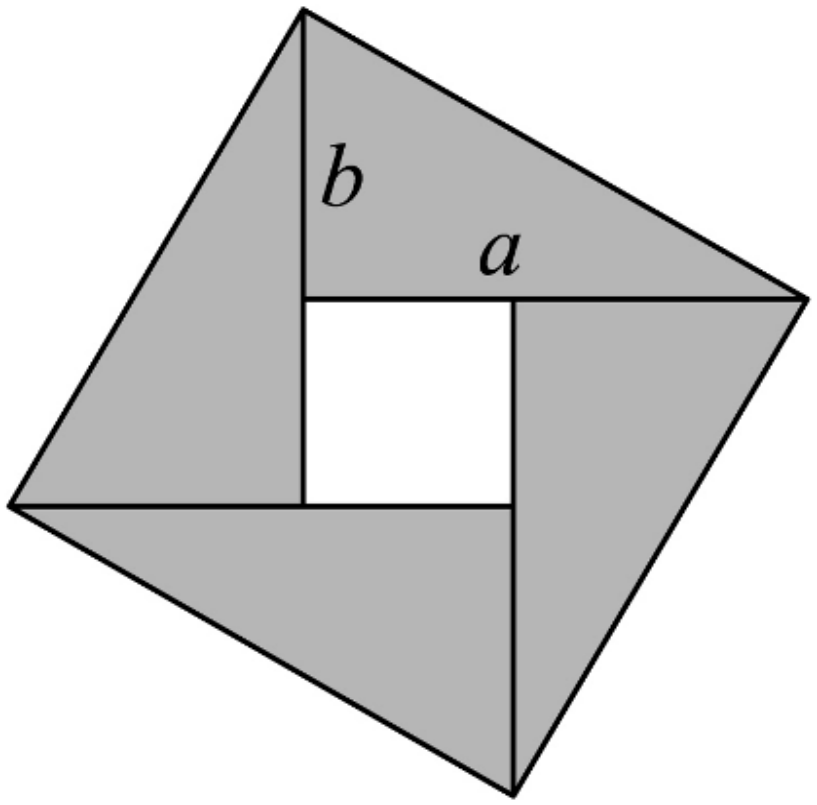
\includegraphics[width=0.20\textwidth]{figures/gao93_q16_zhaoshuang.png}
\end{center}

A. 如果 $a>b>0$，那么 $\sqrt a>\sqrt b$

B. 如果 $a>b>0$，那么 $a^2>b^2$

C. 对任意正实数 $a$ 和 $b$，有 $a^2+b^2\geqslant2ab$，当且仅当 $a=b$ 时等号成立

D. 对任意正实数 $a$ 和 $b$，有 $a^2+b^2\geqslant2ab$，当且仅当 $a=b$ 时等号成立% 原卷 C、D 两选项文字相同，照录

\ifanswer
\solbegin
\step{通过观察，可以发现这个图中的四个直角三角形是全等的，}
\step{设直角三角形的长直角边为 $a$，短直角边为 $b$，}
\step{如图，整个大正方形的面积大于等于这 $4$ 个直角三角形的面积和，}
\step{即 $a^2+b^2\geqslant4\times\left(\dfrac12ab\right)$，即 $a^2+b^2\geqslant2ab$，}
\step{当 $a=b$ 时，中间空白的正方形消失，即整个大正方形与 $4$ 个直角三角形重合；}
\step{其他选项通过该图无法证明. 故选 $C$.}
\solend
\fi

\end{enumerate}

\bigsec{三、解答题}

\begin{enumerate}
\setcounter{enumi}{16}

\item 已知 $x,y\in R$，比较 $x^2+y^2$ 与 $2(2x-y)-5$ 的大小.

\ansspace*[7]

\ifanswer
\solbegin
\step{因为 $x^2+y^2-2(2x-y)+5=(x-2)^2+(y+1)^2\geqslant0$，}
\step{所以 $x^2+y^2\geqslant2(2x-y)-5$.}
\solend
\fi

\item 设 $k\in\R$，求关于 $x$ 与 $y$ 的二元一次方程组 $\begin{cases}y=x+1\\ y=kx+3\end{cases}$ 的解集.

\ansspace*[9]

\ifanswer
\solbegin
\step{因为 $\begin{cases}y=x+1\\ y=kx+3\end{cases}$，两式相减，得到 $(k-1)x=-2$，}
\step{当 $k\neq1$ 时，$x=-\dfrac{2}{k-1}$，代入方程组中的第一式，得到 $y=\dfrac{k-3}{k-1}$，}
\step{此时，原方程组的解集为 $\left\{\left(-\dfrac{2}{k-1},\dfrac{k-3}{k-1}\right)\right\}$，}
\step{当 $k=1$ 时，方程 $(k-1)x=-2$ 无解，从而原方程组无解，其解集为空集.}
\step{综上，当 $k\neq1$ 时，解集为 $\left\{\left(-\dfrac{2}{k-1},\dfrac{k-3}{k-1}\right)\right\}$，}
\step{当 $k=1$ 时，解集为空集.}
\solend
\fi

\item 解下列不等式与方程组.

（1）解含绝对值的不等式：$\lvert x+1\rvert\geqslant3x$；

（2）求解不等式组 $\begin{cases}x^2-4x+3\geqslant0\\ \dfrac{x+3}{2x-1}\geqslant2\end{cases}$.

\ansspace*[10]

\ifanswer
\solbegin
\stepm{（1）}{当 $x\leqslant0$ 时，不等式显然成立，}
\step{当 $x>0$ 时，则 $(x+1)^2\geqslant9x^2$，得 $8x^2-2x-1\leqslant0$，}
\step{得 $(2x-1)(4x+1)\leqslant0$，解得 $-\dfrac14\leqslant x\leqslant\dfrac12$，由于 $x>0$，得 $0<x\leqslant\dfrac12$，}
\step{综上，不等式解集为 $\left\{x\left|x\leqslant\dfrac12\right.\right\}$.}
\stepm{（2）}{由 $x^2-4x+3\geqslant0$ 得 $(x-1)(x-3)\geqslant0$，所以 $x\leqslant1$ 或 $x\geqslant3$；}
\step{由 $\dfrac{x+3}{2x-1}\geqslant2$，得 $\dfrac{x+3}{2x-1}-2=\dfrac{-3x+5}{2x-1}\geqslant0$，即 $\dfrac{3x-5}{2x-1}\leqslant0$，}
\step{所以 $\begin{cases}(3x-5)(2x-1)\leqslant0\\ 2x-1\neq0\end{cases}$，解得 $\dfrac12<x\leqslant\dfrac53$，}
\step{所以不等式组的解集是 $\left\{x\left|\dfrac12<x\leqslant1\right.\right\}$.}
\solend
\fi

\item 已知关于 $x$ 的不等式 $2kx^2+kx-1<0$.

（1）若不等式的解集为 $\left(-\dfrac32,1\right)$，求实数 $k$ 的值；

（2）若不等式的解集为 $R$，求实数 $k$ 的取值范围.

\ansspace*[11]

\ifanswer
\solbegin
\stepm{（1）}{关于 $x$ 的不等式 $2kx^2+kx-1<0$ 的解集为 $\left(-\dfrac32,1\right)$，}
\step{所以 $-\dfrac32$ 和 $1$ 是方程 $2kx^2+kx-1=0$ 的两个实数根，}
\step{代入 $x=1$ 得 $2k+k-1=0$，解得 $k=\dfrac13$；}
\stepm{（2）}{若不等式 $2kx^2+kx-1<0$ 的解集为 $R$，}
\step{则 $k=0$ 时，不等式为 $-1<0$，满足题意；}
\step{$k\neq0$ 时，应满足 $\begin{cases}k<0\\ \Delta=k^2+8k<0\end{cases}$，解得 $-8<k<0$；}
\step{综上，实数 $k$ 的取值范围是 $-8<k\leqslant0$.}
\solend
\fi

\item 国家为了加强对烟酒生产的宏观管理，实行征收附加税政策，现知某种酒每瓶 $70$ 元，不征收附加税的时候，每年大约产销 $100$ 万瓶，若政府征收附加税，每销售 $100$ 元要征税 $R$ 元（叫做税率 $R\%$），则每年的销售将减少 $10R$ 万瓶.

（1）求出每年商店经营烟酒被征收的附加税税金 $S$（单位：万元）；

（2）若附加税税金 $S$ 不少于 $112$ 万元，且不大于 $168$ 万元，求 $R$ 的取值范围.

\ansspace*[12]

\ifanswer
\solbegin
\stepm{（1）}{由题意得 $S=70\times(100-10R)\times R\%(0\leqslant R\leqslant10)$（单位：万元）.}
\stepm{（2）}{由题意 $\begin{cases}70\times(100-10R)\times R\%\geqslant112\\ 70\times(100-10R)\times R\%\leqslant168\end{cases}$，解得 $2\leqslant R\leqslant4$ 或 $6\leqslant R\leqslant8$，}
\step{所以 $R$ 的取值范围是 $[2,4]\cup[6,8]$.}
\solend
\fi

\end{enumerate}

\end{document}
"
% 紧凑版：xelatex "\def\iscompact{1}% 高一93_建平世纪_10月月考.tex
%   —— 高一上数学“2026-2027 年建平世纪高一上 10 月月考”（讲评版）
% 试卷版：xelatex 高一93_建平世纪_10月月考.tex
% 答案版：xelatex "\def\isanswer{1}% 高一93_建平世纪_10月月考.tex
%   —— 高一上数学“2026-2027 年建平世纪高一上 10 月月考”（讲评版）
% 试卷版：xelatex 高一93_建平世纪_10月月考.tex
% 答案版：xelatex "\def\isanswer{1}\input{高一93_建平世纪_10月月考.tex}"
% 紧凑版：xelatex "\def\iscompact{1}\input{高一93_建平世纪_10月月考.tex}"
%
% 原始材料：微信公众号“魔都数学加油站”文章，连载“27学年高一93”；
% 原文标题“27学年高一93——2026-2027年上海市建平世纪高一上10月月考”；
% 原文链接：https://mp.weixin.qq.com/s/uqySZX3I8Q-QZ2J8MqmWiA。
% 正文为 7 张 PNG 页（`原图/高一93_建平世纪_10月月考/01..07.png`），均 4762×6735，按页序读取。
%
% 篇幅与题号：原卷自第 3 题起编号（第 1、2 题不在原文内）。填空题 3—12（10 题）、
% 选择题 13—16（4 题）、解答题 17—21（5 题），共 19 题。
%
% 讲评版：第 3、4 题只印【答案】（“$\{x\mid-1<x<1\}$”“$x$ 和 $y$ 不都是有理数”），本稿只给 \ans{}；
% 其余 17 题印【解析】，其中选择题答案在解析末句“故选 $D$／$D$／$C$／$C$”。
% 第 16 题题干右侧有一幅赵爽弦图（裁自第 4 页原图、去粉色水印后转灰度）。
%
% 副标题：原卷未印副标题。本稿按内容标作“集合与常用逻辑用语、不等式”。
%
% 原卷笔误/存疑（均照录未改，正文对应处另有 % 注）：
%   ① 第 3 题答案印作 $\{x\mid-1<x<1\}$（两端开），而 $\lvert x\rvert\leqslant1$ 的解集应为
%      $[-1,1]$（两端闭）；原卷照录，未改；
%   ② 第 16 题 C、D 两个选项**文字完全相同**（皆为“对任意正实数 $a$ 和 $b$，有
%      $a^2+b^2\geqslant2ab$，当且仅当 $a=b$ 时等号成立”），原卷重复排印；答案取 $C$，
%      本稿两个选项照录。
%
% 与原卷的排版差异：
%   ① 原卷每题下直接印【答案】/【解析】，本稿按全稿惯例将答案与解析置于答案版；
%   ② 原卷未印副标题，本稿补出；填空横线统一排 \blankline[4.4em]；
%   ③ 原卷数集记号排斜体 $R$，本稿按全稿惯例改用 $\R$；
%   ④ 第 17—21 题的子问用行内“（1）（2）（3）”段，解析中的子问标号用 \stepm；
%   ⑤ 解答题按惯例加 \ansspace；选择题括号排 \mbox{（\quad）}；
%   ⑥ 第 16 题的弦图原卷排在题干右侧、文字绕排，本稿改排为选项后的居中图。
%
% 行数核对：逐题数 \step/\stepm 条数，合计 71 条（Q3：0；Q4：0；Q5：2；Q6：3；Q7：2；
% Q8：2；Q9：4；Q10：1；Q11：3；Q12：9；Q13：5；Q14：3；Q15：5；Q16：6；Q17：2；
% Q18：6；Q19：8；Q20：7；Q21：3）。第 3、4 题只印答案，不计入 \step 账。
% 原卷解析的换行按语意合并，未逐行强拆。
%
\documentclass[a4paper,11pt]{article}
\usepackage{common}

\begin{document}

\examtitlest[7]{2026--2027 年建平世纪高一上 10 月月考}{集合与常用逻辑用语、不等式}

\bigsec{一、填空题}

\begin{enumerate}
\setcounter{enumi}{2}

\item 不等式 $\lvert x\rvert\leqslant1$ 的解集是\blankline[4.4em].

\ifanswer
\ans{$\{x\mid-1<x<1\}$}% 原卷答案两端开；|x|≤1 应为 [-1,1]，照录
\fi

\item “$x$ 和 $y$ 都是有理数”的否定形式是\blankline[4.4em].

\ifanswer
\ans{$x$ 和 $y$ 不都是有理数}
\fi

\item 已知等式 $2x^2+3x+5=2ax^2+a(3x+1)+c$ 恒成立，则 $a+c=\blankline[4.4em]$.

\ifanswer
\solbegin
\step{因为 $2x^2+3x+5=2ax^2+a(3x+1)+c$ 恒成立，}
\step{即 $2x^2+3x+5=2ax^2+3ax+(a+c)$ 恒成立，所以 $\begin{cases}2=2a\\ 3=3a\\ 5=a+c\end{cases}$，所以 $a+c=5$.}
\solend
\fi

\item 已知方程 $x^2+6x+m=0(m\in\R)$ 的两个根 $x_1$、$x_2$ 满足 $\lvert x_1-x_2\rvert=4$，则 $m$ 的值是\blankline[4.4em].

\ifanswer
\solbegin
\step{方程 $x^2+6x+m=0(m\in\R)$ 的两根为 $x_1$、$x_2$，所以 $x_1+x_2=-6$，$x_1x_2=m$，}
\step{又 $\lvert x_1-x_2\rvert=4$，则 $(x_1-x_2)^2=(x_1+x_2)^2-4x_1x_2=16$，}
\step{即 $(-6)^2-4m=16$，解得 $m=5$，检验得 $\Delta=6^2-4\times1\times5=16>0$，符合题意，所以 $m=5$.}
\solend
\fi

\item 已知 $\alpha:2m-6<x<m+5$，$\beta:-3<x<5$，若 $\alpha$ 是 $\beta$ 的必要条件，则实数 $m$ 的取值范围是\blankline[4.4em].

\ifanswer
\solbegin
\step{因为 $\alpha$ 是 $\beta$ 的必要条件，所以 $\begin{cases}2m-6\leqslant-3\\ m+5\geqslant5\\ 2m-6<m+5\end{cases}\Rightarrow0\leqslant m\leqslant\dfrac32$，}
\step{所以实数 $m$ 的取值范围是 $\left[0,\dfrac32\right]$.}
\solend
\fi

\item 已知 $-2\leqslant a\leqslant3$，$2\leqslant b\leqslant\dfrac72$，则 $a-2b$ 的取值范围为\blankline[4.4em].

\ifanswer
\solbegin
\step{因为 $-2\leqslant a\leqslant3$，$2\leqslant b\leqslant\dfrac72$，所以 $-7\leqslant-2b\leqslant-4$，所以 $-9\leqslant a-2b\leqslant-1$，}
\step{故 $a-2b$ 的取值范围为 $[-9,-1]$.}
\solend
\fi

\item 已知 $\lvert x+3\rvert+\lvert5-x\rvert>10$，则实数 $x$ 的取值范围为\blankline[4.4em].

\ifanswer
\solbegin
\step{当 $x<-3$ 时，则 $-x-3+5-x>10$，解得 $x<-4$，}
\step{当 $-3\leqslant x\leqslant5$ 时，则 $x+3+5-x=8<10$，原不等式不成立，}
\step{当 $x>5$ 时，则 $x+3+x-5>10$，解得 $x>6$，}
\step{综上所述，实数 $x$ 的取值范围为 $(-\infty,-4)\cup(6,+\infty)$.}
\solend
\fi

\item 已知集合 $A=\{(x,y)\mid y=x+1\}$，$B=\{(x,y)\mid y=-x+3\}$，则 $A\cap B=\blankline[4.4em]$.

\ifanswer
\solbegin
\step{联立 $\begin{cases}y=x+1\\ y=-x+3\end{cases}$，解得 $x=1$，$y=2$，故 $A\cap B=\{(1,2)\}$.}
\solend
\fi

\item 若关于 $x$ 的不等式组 $\begin{cases}\dfrac{x-1}{x-3}<0\\ x>a\end{cases}$ 的解集为空集，则实数 $a$ 的取值范围为\blankline[4.4em].

\ifanswer
\solbegin
\step{$\dfrac{x-1}{x-3}<0$ 等价于 $(x-1)(x-3)<0$，得 $1<x<3$，}
\step{因为 $\begin{cases}\dfrac{x-1}{x-3}<0\\ x>a\end{cases}$ 的解集为空集，}
\step{所以 $a\geqslant3$，故实数 $a$ 的取值范围为 $[3,+\infty)$.}
\solend
\fi

\item 已知由自然数组成的 $n-1$ 个元素的集合 $A=\{1,2,3,4,\cdots,n-1\}(n>1)$，非空集合 $B\subseteq A$，且对任意的 $a\in B$，都有 $n-a\in B$. 当 $n=9$ 时，则所有满足条件的集合 $B$ 的元素的和为\blankline[4.4em].

\ifanswer
\solbegin
\step{当 $n=9$ 时，$A=\{1,2,3,4,5,6,7,8\}$，}
\step{当 $B$ 中有两个元素时，集合 $B$ 可以为 $\{1,8\},\{2,7\},\{3,6\},\{4,5\}$，}
\step{元素总和为 $4\times9=36$；}
\step{当 $B$ 中有四个元素时，集合 $B$ 可以为 $\{1,8\},\{2,7\},\{3,6\},\{4,5\}$ 中任取两个的并集，}
\step{集合 $B$ 共有 $6$ 种情况，元素总和为 $6\times2\times9=108$；}
\step{当 $B$ 中有六个元素时，集合 $B$ 可以为 $\{1,8\},\{2,7\},\{3,6\},\{4,5\}$ 中任取三个的并集，}
\step{集合 $B$ 共有 $4$ 种情况，元素总和为 $4\times3\times9=12\times9=108$；}
\step{当 $B$ 中有八个元素时，$B=\{1,2,3,4,5,6,7,8\}$，元素之和为 $4\times9=36$，}
\step{所以所有满足条件的集合 $B$ 的元素总和为 $36+108+108+36=288$.}
\solend
\fi

\end{enumerate}

\bigsec{二、选择题}

\begin{enumerate}
\setcounter{enumi}{12}

\item 下列说法正确的是\mbox{（\quad）}

\keepwithprev
A. 若 $a>b$，则 $\dfrac1a<\dfrac1b$\qquad B. 若 $a>b,c>d$，则 $ac>bd$

C. 若 $a>b$，则 $ac^2>bc^2$\qquad D. 若 $ac^2>bc^2$，则 $a>b$

\ifanswer
\solbegin
\step{A：令 $a=2,b=-1$，此时 $\dfrac12>-1$，故 A 错误；}
\step{B：令 $a=2,b=-1,c=0,d=-2$，此时 $ac=0<bd=2$，故 B 错误；}
\step{C：由 $a>b$，当 $c=0$ 时，$ac^2=bc^2$，故 C 错误；}
\step{D：由 $ac^2>bc^2$，则 $c^2>0$，所以 $a>b$，故 D 正确.}
\step{故选 $D$.}
\solend
\fi

\item 不等式 $\dfrac{x-3}{x-1}\leqslant2$ 的解集是\mbox{（\quad）}

\keepwithprev
A. $(-\infty,1]$\qquad B. $[1,+\infty)$

C. $(-\infty,-1]\cup[1,+\infty)$\qquad D. $(-\infty,-1]\cup(1,+\infty)$

\ifanswer
\solbegin
\step{不等式 $\dfrac{x-3}{x-1}\leqslant2$ 可化为 $\dfrac{x-3}{x-1}-2\leqslant0$，即 $\dfrac{x-3-2(x-1)}{x-1}\leqslant0$，}
\step{化简得 $\dfrac{x+1}{x-1}\geqslant0$，等价于 $\begin{cases}(x+1)(x-1)\geqslant0\\ x\neq1\end{cases}$，解得 $x\leqslant-1$ 或 $x>1$，}
\step{所以不等式的解集为 $(-\infty,-1]\cup(1,+\infty)$. 故选 $D$.}
\solend
\fi

\item 已知集合 $M$ 和集合 $N$，那么 $M\cap N=N$ 的充要条件是\mbox{（\quad）}

\keepwithprev
A. $M\subseteq N$\qquad B. $N\subset M$\qquad C. $M\supseteq N$\qquad D. $M=N$

\ifanswer
\solbegin
\step{若 $M\subseteq N$，即集合 $M$ 是集合 $N$ 的子集，则 $M\cap N=M$，故 $A$ 错误；}
\step{若 $M=N$，则不能得到 $N\subset M$，故 $B$ 错误；}
\step{若 $M\cap N=N$，则 $M\supseteq N$，故 $C$ 正确；}
\step{当 $N$ 是 $M$ 真子集时，不能得到 $M=N$，故 $D$ 错误.}
\step{故选 $C$.}
\solend
\fi

\item 三国时期赵爽在《勾股方圆图注》中对勾股定理的证明可用现代数学表述为如图所示，我们教材中利用该图作为“（\quad）”的几何解释.

\begin{center}
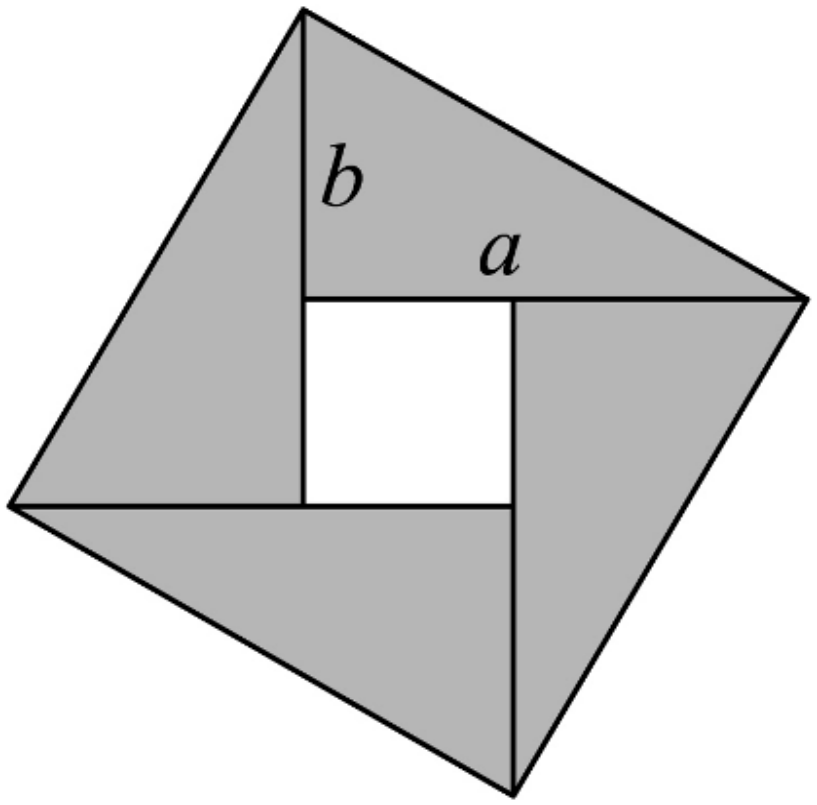
\includegraphics[width=0.20\textwidth]{figures/gao93_q16_zhaoshuang.png}
\end{center}

A. 如果 $a>b>0$，那么 $\sqrt a>\sqrt b$

B. 如果 $a>b>0$，那么 $a^2>b^2$

C. 对任意正实数 $a$ 和 $b$，有 $a^2+b^2\geqslant2ab$，当且仅当 $a=b$ 时等号成立

D. 对任意正实数 $a$ 和 $b$，有 $a^2+b^2\geqslant2ab$，当且仅当 $a=b$ 时等号成立% 原卷 C、D 两选项文字相同，照录

\ifanswer
\solbegin
\step{通过观察，可以发现这个图中的四个直角三角形是全等的，}
\step{设直角三角形的长直角边为 $a$，短直角边为 $b$，}
\step{如图，整个大正方形的面积大于等于这 $4$ 个直角三角形的面积和，}
\step{即 $a^2+b^2\geqslant4\times\left(\dfrac12ab\right)$，即 $a^2+b^2\geqslant2ab$，}
\step{当 $a=b$ 时，中间空白的正方形消失，即整个大正方形与 $4$ 个直角三角形重合；}
\step{其他选项通过该图无法证明. 故选 $C$.}
\solend
\fi

\end{enumerate}

\bigsec{三、解答题}

\begin{enumerate}
\setcounter{enumi}{16}

\item 已知 $x,y\in R$，比较 $x^2+y^2$ 与 $2(2x-y)-5$ 的大小.

\ansspace*[7]

\ifanswer
\solbegin
\step{因为 $x^2+y^2-2(2x-y)+5=(x-2)^2+(y+1)^2\geqslant0$，}
\step{所以 $x^2+y^2\geqslant2(2x-y)-5$.}
\solend
\fi

\item 设 $k\in\R$，求关于 $x$ 与 $y$ 的二元一次方程组 $\begin{cases}y=x+1\\ y=kx+3\end{cases}$ 的解集.

\ansspace*[9]

\ifanswer
\solbegin
\step{因为 $\begin{cases}y=x+1\\ y=kx+3\end{cases}$，两式相减，得到 $(k-1)x=-2$，}
\step{当 $k\neq1$ 时，$x=-\dfrac{2}{k-1}$，代入方程组中的第一式，得到 $y=\dfrac{k-3}{k-1}$，}
\step{此时，原方程组的解集为 $\left\{\left(-\dfrac{2}{k-1},\dfrac{k-3}{k-1}\right)\right\}$，}
\step{当 $k=1$ 时，方程 $(k-1)x=-2$ 无解，从而原方程组无解，其解集为空集.}
\step{综上，当 $k\neq1$ 时，解集为 $\left\{\left(-\dfrac{2}{k-1},\dfrac{k-3}{k-1}\right)\right\}$，}
\step{当 $k=1$ 时，解集为空集.}
\solend
\fi

\item 解下列不等式与方程组.

（1）解含绝对值的不等式：$\lvert x+1\rvert\geqslant3x$；

（2）求解不等式组 $\begin{cases}x^2-4x+3\geqslant0\\ \dfrac{x+3}{2x-1}\geqslant2\end{cases}$.

\ansspace*[10]

\ifanswer
\solbegin
\stepm{（1）}{当 $x\leqslant0$ 时，不等式显然成立，}
\step{当 $x>0$ 时，则 $(x+1)^2\geqslant9x^2$，得 $8x^2-2x-1\leqslant0$，}
\step{得 $(2x-1)(4x+1)\leqslant0$，解得 $-\dfrac14\leqslant x\leqslant\dfrac12$，由于 $x>0$，得 $0<x\leqslant\dfrac12$，}
\step{综上，不等式解集为 $\left\{x\left|x\leqslant\dfrac12\right.\right\}$.}
\stepm{（2）}{由 $x^2-4x+3\geqslant0$ 得 $(x-1)(x-3)\geqslant0$，所以 $x\leqslant1$ 或 $x\geqslant3$；}
\step{由 $\dfrac{x+3}{2x-1}\geqslant2$，得 $\dfrac{x+3}{2x-1}-2=\dfrac{-3x+5}{2x-1}\geqslant0$，即 $\dfrac{3x-5}{2x-1}\leqslant0$，}
\step{所以 $\begin{cases}(3x-5)(2x-1)\leqslant0\\ 2x-1\neq0\end{cases}$，解得 $\dfrac12<x\leqslant\dfrac53$，}
\step{所以不等式组的解集是 $\left\{x\left|\dfrac12<x\leqslant1\right.\right\}$.}
\solend
\fi

\item 已知关于 $x$ 的不等式 $2kx^2+kx-1<0$.

（1）若不等式的解集为 $\left(-\dfrac32,1\right)$，求实数 $k$ 的值；

（2）若不等式的解集为 $R$，求实数 $k$ 的取值范围.

\ansspace*[11]

\ifanswer
\solbegin
\stepm{（1）}{关于 $x$ 的不等式 $2kx^2+kx-1<0$ 的解集为 $\left(-\dfrac32,1\right)$，}
\step{所以 $-\dfrac32$ 和 $1$ 是方程 $2kx^2+kx-1=0$ 的两个实数根，}
\step{代入 $x=1$ 得 $2k+k-1=0$，解得 $k=\dfrac13$；}
\stepm{（2）}{若不等式 $2kx^2+kx-1<0$ 的解集为 $R$，}
\step{则 $k=0$ 时，不等式为 $-1<0$，满足题意；}
\step{$k\neq0$ 时，应满足 $\begin{cases}k<0\\ \Delta=k^2+8k<0\end{cases}$，解得 $-8<k<0$；}
\step{综上，实数 $k$ 的取值范围是 $-8<k\leqslant0$.}
\solend
\fi

\item 国家为了加强对烟酒生产的宏观管理，实行征收附加税政策，现知某种酒每瓶 $70$ 元，不征收附加税的时候，每年大约产销 $100$ 万瓶，若政府征收附加税，每销售 $100$ 元要征税 $R$ 元（叫做税率 $R\%$），则每年的销售将减少 $10R$ 万瓶.

（1）求出每年商店经营烟酒被征收的附加税税金 $S$（单位：万元）；

（2）若附加税税金 $S$ 不少于 $112$ 万元，且不大于 $168$ 万元，求 $R$ 的取值范围.

\ansspace*[12]

\ifanswer
\solbegin
\stepm{（1）}{由题意得 $S=70\times(100-10R)\times R\%(0\leqslant R\leqslant10)$（单位：万元）.}
\stepm{（2）}{由题意 $\begin{cases}70\times(100-10R)\times R\%\geqslant112\\ 70\times(100-10R)\times R\%\leqslant168\end{cases}$，解得 $2\leqslant R\leqslant4$ 或 $6\leqslant R\leqslant8$，}
\step{所以 $R$ 的取值范围是 $[2,4]\cup[6,8]$.}
\solend
\fi

\end{enumerate}

\end{document}
"
% 紧凑版：xelatex "\def\iscompact{1}% 高一93_建平世纪_10月月考.tex
%   —— 高一上数学“2026-2027 年建平世纪高一上 10 月月考”（讲评版）
% 试卷版：xelatex 高一93_建平世纪_10月月考.tex
% 答案版：xelatex "\def\isanswer{1}\input{高一93_建平世纪_10月月考.tex}"
% 紧凑版：xelatex "\def\iscompact{1}\input{高一93_建平世纪_10月月考.tex}"
%
% 原始材料：微信公众号“魔都数学加油站”文章，连载“27学年高一93”；
% 原文标题“27学年高一93——2026-2027年上海市建平世纪高一上10月月考”；
% 原文链接：https://mp.weixin.qq.com/s/uqySZX3I8Q-QZ2J8MqmWiA。
% 正文为 7 张 PNG 页（`原图/高一93_建平世纪_10月月考/01..07.png`），均 4762×6735，按页序读取。
%
% 篇幅与题号：原卷自第 3 题起编号（第 1、2 题不在原文内）。填空题 3—12（10 题）、
% 选择题 13—16（4 题）、解答题 17—21（5 题），共 19 题。
%
% 讲评版：第 3、4 题只印【答案】（“$\{x\mid-1<x<1\}$”“$x$ 和 $y$ 不都是有理数”），本稿只给 \ans{}；
% 其余 17 题印【解析】，其中选择题答案在解析末句“故选 $D$／$D$／$C$／$C$”。
% 第 16 题题干右侧有一幅赵爽弦图（裁自第 4 页原图、去粉色水印后转灰度）。
%
% 副标题：原卷未印副标题。本稿按内容标作“集合与常用逻辑用语、不等式”。
%
% 原卷笔误/存疑（均照录未改，正文对应处另有 % 注）：
%   ① 第 3 题答案印作 $\{x\mid-1<x<1\}$（两端开），而 $\lvert x\rvert\leqslant1$ 的解集应为
%      $[-1,1]$（两端闭）；原卷照录，未改；
%   ② 第 16 题 C、D 两个选项**文字完全相同**（皆为“对任意正实数 $a$ 和 $b$，有
%      $a^2+b^2\geqslant2ab$，当且仅当 $a=b$ 时等号成立”），原卷重复排印；答案取 $C$，
%      本稿两个选项照录。
%
% 与原卷的排版差异：
%   ① 原卷每题下直接印【答案】/【解析】，本稿按全稿惯例将答案与解析置于答案版；
%   ② 原卷未印副标题，本稿补出；填空横线统一排 \blankline[4.4em]；
%   ③ 原卷数集记号排斜体 $R$，本稿按全稿惯例改用 $\R$；
%   ④ 第 17—21 题的子问用行内“（1）（2）（3）”段，解析中的子问标号用 \stepm；
%   ⑤ 解答题按惯例加 \ansspace；选择题括号排 \mbox{（\quad）}；
%   ⑥ 第 16 题的弦图原卷排在题干右侧、文字绕排，本稿改排为选项后的居中图。
%
% 行数核对：逐题数 \step/\stepm 条数，合计 71 条（Q3：0；Q4：0；Q5：2；Q6：3；Q7：2；
% Q8：2；Q9：4；Q10：1；Q11：3；Q12：9；Q13：5；Q14：3；Q15：5；Q16：6；Q17：2；
% Q18：6；Q19：8；Q20：7；Q21：3）。第 3、4 题只印答案，不计入 \step 账。
% 原卷解析的换行按语意合并，未逐行强拆。
%
\documentclass[a4paper,11pt]{article}
\usepackage{common}

\begin{document}

\examtitlest[7]{2026--2027 年建平世纪高一上 10 月月考}{集合与常用逻辑用语、不等式}

\bigsec{一、填空题}

\begin{enumerate}
\setcounter{enumi}{2}

\item 不等式 $\lvert x\rvert\leqslant1$ 的解集是\blankline[4.4em].

\ifanswer
\ans{$\{x\mid-1<x<1\}$}% 原卷答案两端开；|x|≤1 应为 [-1,1]，照录
\fi

\item “$x$ 和 $y$ 都是有理数”的否定形式是\blankline[4.4em].

\ifanswer
\ans{$x$ 和 $y$ 不都是有理数}
\fi

\item 已知等式 $2x^2+3x+5=2ax^2+a(3x+1)+c$ 恒成立，则 $a+c=\blankline[4.4em]$.

\ifanswer
\solbegin
\step{因为 $2x^2+3x+5=2ax^2+a(3x+1)+c$ 恒成立，}
\step{即 $2x^2+3x+5=2ax^2+3ax+(a+c)$ 恒成立，所以 $\begin{cases}2=2a\\ 3=3a\\ 5=a+c\end{cases}$，所以 $a+c=5$.}
\solend
\fi

\item 已知方程 $x^2+6x+m=0(m\in\R)$ 的两个根 $x_1$、$x_2$ 满足 $\lvert x_1-x_2\rvert=4$，则 $m$ 的值是\blankline[4.4em].

\ifanswer
\solbegin
\step{方程 $x^2+6x+m=0(m\in\R)$ 的两根为 $x_1$、$x_2$，所以 $x_1+x_2=-6$，$x_1x_2=m$，}
\step{又 $\lvert x_1-x_2\rvert=4$，则 $(x_1-x_2)^2=(x_1+x_2)^2-4x_1x_2=16$，}
\step{即 $(-6)^2-4m=16$，解得 $m=5$，检验得 $\Delta=6^2-4\times1\times5=16>0$，符合题意，所以 $m=5$.}
\solend
\fi

\item 已知 $\alpha:2m-6<x<m+5$，$\beta:-3<x<5$，若 $\alpha$ 是 $\beta$ 的必要条件，则实数 $m$ 的取值范围是\blankline[4.4em].

\ifanswer
\solbegin
\step{因为 $\alpha$ 是 $\beta$ 的必要条件，所以 $\begin{cases}2m-6\leqslant-3\\ m+5\geqslant5\\ 2m-6<m+5\end{cases}\Rightarrow0\leqslant m\leqslant\dfrac32$，}
\step{所以实数 $m$ 的取值范围是 $\left[0,\dfrac32\right]$.}
\solend
\fi

\item 已知 $-2\leqslant a\leqslant3$，$2\leqslant b\leqslant\dfrac72$，则 $a-2b$ 的取值范围为\blankline[4.4em].

\ifanswer
\solbegin
\step{因为 $-2\leqslant a\leqslant3$，$2\leqslant b\leqslant\dfrac72$，所以 $-7\leqslant-2b\leqslant-4$，所以 $-9\leqslant a-2b\leqslant-1$，}
\step{故 $a-2b$ 的取值范围为 $[-9,-1]$.}
\solend
\fi

\item 已知 $\lvert x+3\rvert+\lvert5-x\rvert>10$，则实数 $x$ 的取值范围为\blankline[4.4em].

\ifanswer
\solbegin
\step{当 $x<-3$ 时，则 $-x-3+5-x>10$，解得 $x<-4$，}
\step{当 $-3\leqslant x\leqslant5$ 时，则 $x+3+5-x=8<10$，原不等式不成立，}
\step{当 $x>5$ 时，则 $x+3+x-5>10$，解得 $x>6$，}
\step{综上所述，实数 $x$ 的取值范围为 $(-\infty,-4)\cup(6,+\infty)$.}
\solend
\fi

\item 已知集合 $A=\{(x,y)\mid y=x+1\}$，$B=\{(x,y)\mid y=-x+3\}$，则 $A\cap B=\blankline[4.4em]$.

\ifanswer
\solbegin
\step{联立 $\begin{cases}y=x+1\\ y=-x+3\end{cases}$，解得 $x=1$，$y=2$，故 $A\cap B=\{(1,2)\}$.}
\solend
\fi

\item 若关于 $x$ 的不等式组 $\begin{cases}\dfrac{x-1}{x-3}<0\\ x>a\end{cases}$ 的解集为空集，则实数 $a$ 的取值范围为\blankline[4.4em].

\ifanswer
\solbegin
\step{$\dfrac{x-1}{x-3}<0$ 等价于 $(x-1)(x-3)<0$，得 $1<x<3$，}
\step{因为 $\begin{cases}\dfrac{x-1}{x-3}<0\\ x>a\end{cases}$ 的解集为空集，}
\step{所以 $a\geqslant3$，故实数 $a$ 的取值范围为 $[3,+\infty)$.}
\solend
\fi

\item 已知由自然数组成的 $n-1$ 个元素的集合 $A=\{1,2,3,4,\cdots,n-1\}(n>1)$，非空集合 $B\subseteq A$，且对任意的 $a\in B$，都有 $n-a\in B$. 当 $n=9$ 时，则所有满足条件的集合 $B$ 的元素的和为\blankline[4.4em].

\ifanswer
\solbegin
\step{当 $n=9$ 时，$A=\{1,2,3,4,5,6,7,8\}$，}
\step{当 $B$ 中有两个元素时，集合 $B$ 可以为 $\{1,8\},\{2,7\},\{3,6\},\{4,5\}$，}
\step{元素总和为 $4\times9=36$；}
\step{当 $B$ 中有四个元素时，集合 $B$ 可以为 $\{1,8\},\{2,7\},\{3,6\},\{4,5\}$ 中任取两个的并集，}
\step{集合 $B$ 共有 $6$ 种情况，元素总和为 $6\times2\times9=108$；}
\step{当 $B$ 中有六个元素时，集合 $B$ 可以为 $\{1,8\},\{2,7\},\{3,6\},\{4,5\}$ 中任取三个的并集，}
\step{集合 $B$ 共有 $4$ 种情况，元素总和为 $4\times3\times9=12\times9=108$；}
\step{当 $B$ 中有八个元素时，$B=\{1,2,3,4,5,6,7,8\}$，元素之和为 $4\times9=36$，}
\step{所以所有满足条件的集合 $B$ 的元素总和为 $36+108+108+36=288$.}
\solend
\fi

\end{enumerate}

\bigsec{二、选择题}

\begin{enumerate}
\setcounter{enumi}{12}

\item 下列说法正确的是\mbox{（\quad）}

\keepwithprev
A. 若 $a>b$，则 $\dfrac1a<\dfrac1b$\qquad B. 若 $a>b,c>d$，则 $ac>bd$

C. 若 $a>b$，则 $ac^2>bc^2$\qquad D. 若 $ac^2>bc^2$，则 $a>b$

\ifanswer
\solbegin
\step{A：令 $a=2,b=-1$，此时 $\dfrac12>-1$，故 A 错误；}
\step{B：令 $a=2,b=-1,c=0,d=-2$，此时 $ac=0<bd=2$，故 B 错误；}
\step{C：由 $a>b$，当 $c=0$ 时，$ac^2=bc^2$，故 C 错误；}
\step{D：由 $ac^2>bc^2$，则 $c^2>0$，所以 $a>b$，故 D 正确.}
\step{故选 $D$.}
\solend
\fi

\item 不等式 $\dfrac{x-3}{x-1}\leqslant2$ 的解集是\mbox{（\quad）}

\keepwithprev
A. $(-\infty,1]$\qquad B. $[1,+\infty)$

C. $(-\infty,-1]\cup[1,+\infty)$\qquad D. $(-\infty,-1]\cup(1,+\infty)$

\ifanswer
\solbegin
\step{不等式 $\dfrac{x-3}{x-1}\leqslant2$ 可化为 $\dfrac{x-3}{x-1}-2\leqslant0$，即 $\dfrac{x-3-2(x-1)}{x-1}\leqslant0$，}
\step{化简得 $\dfrac{x+1}{x-1}\geqslant0$，等价于 $\begin{cases}(x+1)(x-1)\geqslant0\\ x\neq1\end{cases}$，解得 $x\leqslant-1$ 或 $x>1$，}
\step{所以不等式的解集为 $(-\infty,-1]\cup(1,+\infty)$. 故选 $D$.}
\solend
\fi

\item 已知集合 $M$ 和集合 $N$，那么 $M\cap N=N$ 的充要条件是\mbox{（\quad）}

\keepwithprev
A. $M\subseteq N$\qquad B. $N\subset M$\qquad C. $M\supseteq N$\qquad D. $M=N$

\ifanswer
\solbegin
\step{若 $M\subseteq N$，即集合 $M$ 是集合 $N$ 的子集，则 $M\cap N=M$，故 $A$ 错误；}
\step{若 $M=N$，则不能得到 $N\subset M$，故 $B$ 错误；}
\step{若 $M\cap N=N$，则 $M\supseteq N$，故 $C$ 正确；}
\step{当 $N$ 是 $M$ 真子集时，不能得到 $M=N$，故 $D$ 错误.}
\step{故选 $C$.}
\solend
\fi

\item 三国时期赵爽在《勾股方圆图注》中对勾股定理的证明可用现代数学表述为如图所示，我们教材中利用该图作为“（\quad）”的几何解释.

\begin{center}
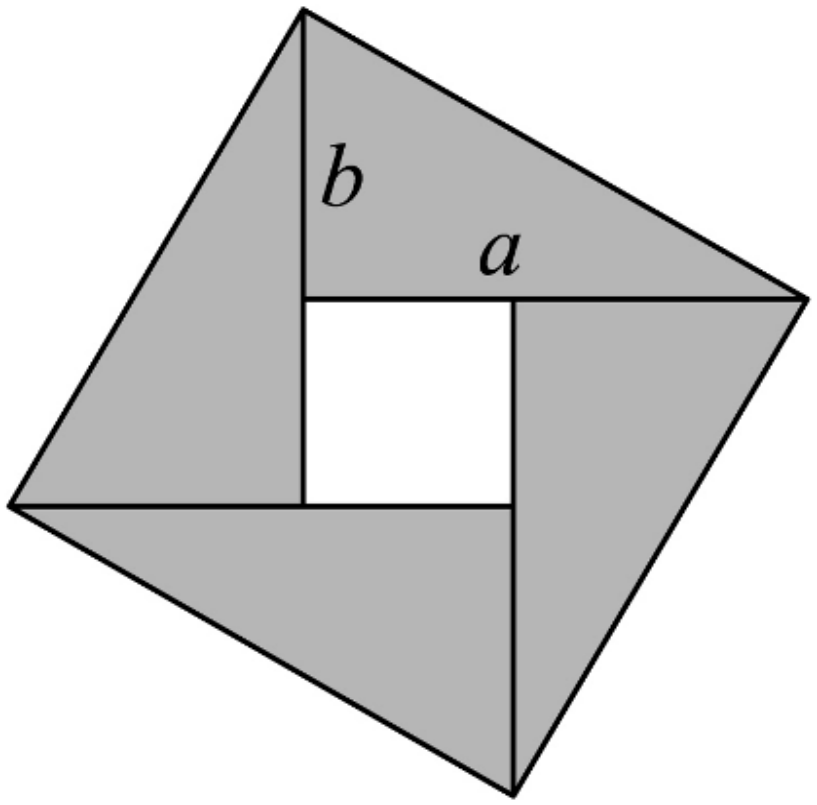
\includegraphics[width=0.20\textwidth]{figures/gao93_q16_zhaoshuang.png}
\end{center}

A. 如果 $a>b>0$，那么 $\sqrt a>\sqrt b$

B. 如果 $a>b>0$，那么 $a^2>b^2$

C. 对任意正实数 $a$ 和 $b$，有 $a^2+b^2\geqslant2ab$，当且仅当 $a=b$ 时等号成立

D. 对任意正实数 $a$ 和 $b$，有 $a^2+b^2\geqslant2ab$，当且仅当 $a=b$ 时等号成立% 原卷 C、D 两选项文字相同，照录

\ifanswer
\solbegin
\step{通过观察，可以发现这个图中的四个直角三角形是全等的，}
\step{设直角三角形的长直角边为 $a$，短直角边为 $b$，}
\step{如图，整个大正方形的面积大于等于这 $4$ 个直角三角形的面积和，}
\step{即 $a^2+b^2\geqslant4\times\left(\dfrac12ab\right)$，即 $a^2+b^2\geqslant2ab$，}
\step{当 $a=b$ 时，中间空白的正方形消失，即整个大正方形与 $4$ 个直角三角形重合；}
\step{其他选项通过该图无法证明. 故选 $C$.}
\solend
\fi

\end{enumerate}

\bigsec{三、解答题}

\begin{enumerate}
\setcounter{enumi}{16}

\item 已知 $x,y\in R$，比较 $x^2+y^2$ 与 $2(2x-y)-5$ 的大小.

\ansspace*[7]

\ifanswer
\solbegin
\step{因为 $x^2+y^2-2(2x-y)+5=(x-2)^2+(y+1)^2\geqslant0$，}
\step{所以 $x^2+y^2\geqslant2(2x-y)-5$.}
\solend
\fi

\item 设 $k\in\R$，求关于 $x$ 与 $y$ 的二元一次方程组 $\begin{cases}y=x+1\\ y=kx+3\end{cases}$ 的解集.

\ansspace*[9]

\ifanswer
\solbegin
\step{因为 $\begin{cases}y=x+1\\ y=kx+3\end{cases}$，两式相减，得到 $(k-1)x=-2$，}
\step{当 $k\neq1$ 时，$x=-\dfrac{2}{k-1}$，代入方程组中的第一式，得到 $y=\dfrac{k-3}{k-1}$，}
\step{此时，原方程组的解集为 $\left\{\left(-\dfrac{2}{k-1},\dfrac{k-3}{k-1}\right)\right\}$，}
\step{当 $k=1$ 时，方程 $(k-1)x=-2$ 无解，从而原方程组无解，其解集为空集.}
\step{综上，当 $k\neq1$ 时，解集为 $\left\{\left(-\dfrac{2}{k-1},\dfrac{k-3}{k-1}\right)\right\}$，}
\step{当 $k=1$ 时，解集为空集.}
\solend
\fi

\item 解下列不等式与方程组.

（1）解含绝对值的不等式：$\lvert x+1\rvert\geqslant3x$；

（2）求解不等式组 $\begin{cases}x^2-4x+3\geqslant0\\ \dfrac{x+3}{2x-1}\geqslant2\end{cases}$.

\ansspace*[10]

\ifanswer
\solbegin
\stepm{（1）}{当 $x\leqslant0$ 时，不等式显然成立，}
\step{当 $x>0$ 时，则 $(x+1)^2\geqslant9x^2$，得 $8x^2-2x-1\leqslant0$，}
\step{得 $(2x-1)(4x+1)\leqslant0$，解得 $-\dfrac14\leqslant x\leqslant\dfrac12$，由于 $x>0$，得 $0<x\leqslant\dfrac12$，}
\step{综上，不等式解集为 $\left\{x\left|x\leqslant\dfrac12\right.\right\}$.}
\stepm{（2）}{由 $x^2-4x+3\geqslant0$ 得 $(x-1)(x-3)\geqslant0$，所以 $x\leqslant1$ 或 $x\geqslant3$；}
\step{由 $\dfrac{x+3}{2x-1}\geqslant2$，得 $\dfrac{x+3}{2x-1}-2=\dfrac{-3x+5}{2x-1}\geqslant0$，即 $\dfrac{3x-5}{2x-1}\leqslant0$，}
\step{所以 $\begin{cases}(3x-5)(2x-1)\leqslant0\\ 2x-1\neq0\end{cases}$，解得 $\dfrac12<x\leqslant\dfrac53$，}
\step{所以不等式组的解集是 $\left\{x\left|\dfrac12<x\leqslant1\right.\right\}$.}
\solend
\fi

\item 已知关于 $x$ 的不等式 $2kx^2+kx-1<0$.

（1）若不等式的解集为 $\left(-\dfrac32,1\right)$，求实数 $k$ 的值；

（2）若不等式的解集为 $R$，求实数 $k$ 的取值范围.

\ansspace*[11]

\ifanswer
\solbegin
\stepm{（1）}{关于 $x$ 的不等式 $2kx^2+kx-1<0$ 的解集为 $\left(-\dfrac32,1\right)$，}
\step{所以 $-\dfrac32$ 和 $1$ 是方程 $2kx^2+kx-1=0$ 的两个实数根，}
\step{代入 $x=1$ 得 $2k+k-1=0$，解得 $k=\dfrac13$；}
\stepm{（2）}{若不等式 $2kx^2+kx-1<0$ 的解集为 $R$，}
\step{则 $k=0$ 时，不等式为 $-1<0$，满足题意；}
\step{$k\neq0$ 时，应满足 $\begin{cases}k<0\\ \Delta=k^2+8k<0\end{cases}$，解得 $-8<k<0$；}
\step{综上，实数 $k$ 的取值范围是 $-8<k\leqslant0$.}
\solend
\fi

\item 国家为了加强对烟酒生产的宏观管理，实行征收附加税政策，现知某种酒每瓶 $70$ 元，不征收附加税的时候，每年大约产销 $100$ 万瓶，若政府征收附加税，每销售 $100$ 元要征税 $R$ 元（叫做税率 $R\%$），则每年的销售将减少 $10R$ 万瓶.

（1）求出每年商店经营烟酒被征收的附加税税金 $S$（单位：万元）；

（2）若附加税税金 $S$ 不少于 $112$ 万元，且不大于 $168$ 万元，求 $R$ 的取值范围.

\ansspace*[12]

\ifanswer
\solbegin
\stepm{（1）}{由题意得 $S=70\times(100-10R)\times R\%(0\leqslant R\leqslant10)$（单位：万元）.}
\stepm{（2）}{由题意 $\begin{cases}70\times(100-10R)\times R\%\geqslant112\\ 70\times(100-10R)\times R\%\leqslant168\end{cases}$，解得 $2\leqslant R\leqslant4$ 或 $6\leqslant R\leqslant8$，}
\step{所以 $R$ 的取值范围是 $[2,4]\cup[6,8]$.}
\solend
\fi

\end{enumerate}

\end{document}
"
%
% 原始材料：微信公众号“魔都数学加油站”文章，连载“27学年高一93”；
% 原文标题“27学年高一93——2026-2027年上海市建平世纪高一上10月月考”；
% 原文链接：https://mp.weixin.qq.com/s/uqySZX3I8Q-QZ2J8MqmWiA。
% 正文为 7 张 PNG 页（`原图/高一93_建平世纪_10月月考/01..07.png`），均 4762×6735，按页序读取。
%
% 篇幅与题号：原卷自第 3 题起编号（第 1、2 题不在原文内）。填空题 3—12（10 题）、
% 选择题 13—16（4 题）、解答题 17—21（5 题），共 19 题。
%
% 讲评版：第 3、4 题只印【答案】（“$\{x\mid-1<x<1\}$”“$x$ 和 $y$ 不都是有理数”），本稿只给 \ans{}；
% 其余 17 题印【解析】，其中选择题答案在解析末句“故选 $D$／$D$／$C$／$C$”。
% 第 16 题题干右侧有一幅赵爽弦图（裁自第 4 页原图、去粉色水印后转灰度）。
%
% 副标题：原卷未印副标题。本稿按内容标作“集合与常用逻辑用语、不等式”。
%
% 原卷笔误/存疑（均照录未改，正文对应处另有 % 注）：
%   ① 第 3 题答案印作 $\{x\mid-1<x<1\}$（两端开），而 $\lvert x\rvert\leqslant1$ 的解集应为
%      $[-1,1]$（两端闭）；原卷照录，未改；
%   ② 第 16 题 C、D 两个选项**文字完全相同**（皆为“对任意正实数 $a$ 和 $b$，有
%      $a^2+b^2\geqslant2ab$，当且仅当 $a=b$ 时等号成立”），原卷重复排印；答案取 $C$，
%      本稿两个选项照录。
%
% 与原卷的排版差异：
%   ① 原卷每题下直接印【答案】/【解析】，本稿按全稿惯例将答案与解析置于答案版；
%   ② 原卷未印副标题，本稿补出；填空横线统一排 \blankline[4.4em]；
%   ③ 原卷数集记号排斜体 $R$，本稿按全稿惯例改用 $\R$；
%   ④ 第 17—21 题的子问用行内“（1）（2）（3）”段，解析中的子问标号用 \stepm；
%   ⑤ 解答题按惯例加 \ansspace；选择题括号排 \mbox{（\quad）}；
%   ⑥ 第 16 题的弦图原卷排在题干右侧、文字绕排，本稿改排为选项后的居中图。
%
% 行数核对：逐题数 \step/\stepm 条数，合计 71 条（Q3：0；Q4：0；Q5：2；Q6：3；Q7：2；
% Q8：2；Q9：4；Q10：1；Q11：3；Q12：9；Q13：5；Q14：3；Q15：5；Q16：6；Q17：2；
% Q18：6；Q19：8；Q20：7；Q21：3）。第 3、4 题只印答案，不计入 \step 账。
% 原卷解析的换行按语意合并，未逐行强拆。
%
\documentclass[a4paper,11pt]{article}
\usepackage{common}

\begin{document}

\examtitlest[7]{2026--2027 年建平世纪高一上 10 月月考}{集合与常用逻辑用语、不等式}

\bigsec{一、填空题}

\begin{enumerate}
\setcounter{enumi}{2}

\item 不等式 $\lvert x\rvert\leqslant1$ 的解集是\blankline[4.4em].

\ifanswer
\ans{$\{x\mid-1<x<1\}$}% 原卷答案两端开；|x|≤1 应为 [-1,1]，照录
\fi

\item “$x$ 和 $y$ 都是有理数”的否定形式是\blankline[4.4em].

\ifanswer
\ans{$x$ 和 $y$ 不都是有理数}
\fi

\item 已知等式 $2x^2+3x+5=2ax^2+a(3x+1)+c$ 恒成立，则 $a+c=\blankline[4.4em]$.

\ifanswer
\solbegin
\step{因为 $2x^2+3x+5=2ax^2+a(3x+1)+c$ 恒成立，}
\step{即 $2x^2+3x+5=2ax^2+3ax+(a+c)$ 恒成立，所以 $\begin{cases}2=2a\\ 3=3a\\ 5=a+c\end{cases}$，所以 $a+c=5$.}
\solend
\fi

\item 已知方程 $x^2+6x+m=0(m\in\R)$ 的两个根 $x_1$、$x_2$ 满足 $\lvert x_1-x_2\rvert=4$，则 $m$ 的值是\blankline[4.4em].

\ifanswer
\solbegin
\step{方程 $x^2+6x+m=0(m\in\R)$ 的两根为 $x_1$、$x_2$，所以 $x_1+x_2=-6$，$x_1x_2=m$，}
\step{又 $\lvert x_1-x_2\rvert=4$，则 $(x_1-x_2)^2=(x_1+x_2)^2-4x_1x_2=16$，}
\step{即 $(-6)^2-4m=16$，解得 $m=5$，检验得 $\Delta=6^2-4\times1\times5=16>0$，符合题意，所以 $m=5$.}
\solend
\fi

\item 已知 $\alpha:2m-6<x<m+5$，$\beta:-3<x<5$，若 $\alpha$ 是 $\beta$ 的必要条件，则实数 $m$ 的取值范围是\blankline[4.4em].

\ifanswer
\solbegin
\step{因为 $\alpha$ 是 $\beta$ 的必要条件，所以 $\begin{cases}2m-6\leqslant-3\\ m+5\geqslant5\\ 2m-6<m+5\end{cases}\Rightarrow0\leqslant m\leqslant\dfrac32$，}
\step{所以实数 $m$ 的取值范围是 $\left[0,\dfrac32\right]$.}
\solend
\fi

\item 已知 $-2\leqslant a\leqslant3$，$2\leqslant b\leqslant\dfrac72$，则 $a-2b$ 的取值范围为\blankline[4.4em].

\ifanswer
\solbegin
\step{因为 $-2\leqslant a\leqslant3$，$2\leqslant b\leqslant\dfrac72$，所以 $-7\leqslant-2b\leqslant-4$，所以 $-9\leqslant a-2b\leqslant-1$，}
\step{故 $a-2b$ 的取值范围为 $[-9,-1]$.}
\solend
\fi

\item 已知 $\lvert x+3\rvert+\lvert5-x\rvert>10$，则实数 $x$ 的取值范围为\blankline[4.4em].

\ifanswer
\solbegin
\step{当 $x<-3$ 时，则 $-x-3+5-x>10$，解得 $x<-4$，}
\step{当 $-3\leqslant x\leqslant5$ 时，则 $x+3+5-x=8<10$，原不等式不成立，}
\step{当 $x>5$ 时，则 $x+3+x-5>10$，解得 $x>6$，}
\step{综上所述，实数 $x$ 的取值范围为 $(-\infty,-4)\cup(6,+\infty)$.}
\solend
\fi

\item 已知集合 $A=\{(x,y)\mid y=x+1\}$，$B=\{(x,y)\mid y=-x+3\}$，则 $A\cap B=\blankline[4.4em]$.

\ifanswer
\solbegin
\step{联立 $\begin{cases}y=x+1\\ y=-x+3\end{cases}$，解得 $x=1$，$y=2$，故 $A\cap B=\{(1,2)\}$.}
\solend
\fi

\item 若关于 $x$ 的不等式组 $\begin{cases}\dfrac{x-1}{x-3}<0\\ x>a\end{cases}$ 的解集为空集，则实数 $a$ 的取值范围为\blankline[4.4em].

\ifanswer
\solbegin
\step{$\dfrac{x-1}{x-3}<0$ 等价于 $(x-1)(x-3)<0$，得 $1<x<3$，}
\step{因为 $\begin{cases}\dfrac{x-1}{x-3}<0\\ x>a\end{cases}$ 的解集为空集，}
\step{所以 $a\geqslant3$，故实数 $a$ 的取值范围为 $[3,+\infty)$.}
\solend
\fi

\item 已知由自然数组成的 $n-1$ 个元素的集合 $A=\{1,2,3,4,\cdots,n-1\}(n>1)$，非空集合 $B\subseteq A$，且对任意的 $a\in B$，都有 $n-a\in B$. 当 $n=9$ 时，则所有满足条件的集合 $B$ 的元素的和为\blankline[4.4em].

\ifanswer
\solbegin
\step{当 $n=9$ 时，$A=\{1,2,3,4,5,6,7,8\}$，}
\step{当 $B$ 中有两个元素时，集合 $B$ 可以为 $\{1,8\},\{2,7\},\{3,6\},\{4,5\}$，}
\step{元素总和为 $4\times9=36$；}
\step{当 $B$ 中有四个元素时，集合 $B$ 可以为 $\{1,8\},\{2,7\},\{3,6\},\{4,5\}$ 中任取两个的并集，}
\step{集合 $B$ 共有 $6$ 种情况，元素总和为 $6\times2\times9=108$；}
\step{当 $B$ 中有六个元素时，集合 $B$ 可以为 $\{1,8\},\{2,7\},\{3,6\},\{4,5\}$ 中任取三个的并集，}
\step{集合 $B$ 共有 $4$ 种情况，元素总和为 $4\times3\times9=12\times9=108$；}
\step{当 $B$ 中有八个元素时，$B=\{1,2,3,4,5,6,7,8\}$，元素之和为 $4\times9=36$，}
\step{所以所有满足条件的集合 $B$ 的元素总和为 $36+108+108+36=288$.}
\solend
\fi

\end{enumerate}

\bigsec{二、选择题}

\begin{enumerate}
\setcounter{enumi}{12}

\item 下列说法正确的是\mbox{（\quad）}

\keepwithprev
A. 若 $a>b$，则 $\dfrac1a<\dfrac1b$\qquad B. 若 $a>b,c>d$，则 $ac>bd$

C. 若 $a>b$，则 $ac^2>bc^2$\qquad D. 若 $ac^2>bc^2$，则 $a>b$

\ifanswer
\solbegin
\step{A：令 $a=2,b=-1$，此时 $\dfrac12>-1$，故 A 错误；}
\step{B：令 $a=2,b=-1,c=0,d=-2$，此时 $ac=0<bd=2$，故 B 错误；}
\step{C：由 $a>b$，当 $c=0$ 时，$ac^2=bc^2$，故 C 错误；}
\step{D：由 $ac^2>bc^2$，则 $c^2>0$，所以 $a>b$，故 D 正确.}
\step{故选 $D$.}
\solend
\fi

\item 不等式 $\dfrac{x-3}{x-1}\leqslant2$ 的解集是\mbox{（\quad）}

\keepwithprev
A. $(-\infty,1]$\qquad B. $[1,+\infty)$

C. $(-\infty,-1]\cup[1,+\infty)$\qquad D. $(-\infty,-1]\cup(1,+\infty)$

\ifanswer
\solbegin
\step{不等式 $\dfrac{x-3}{x-1}\leqslant2$ 可化为 $\dfrac{x-3}{x-1}-2\leqslant0$，即 $\dfrac{x-3-2(x-1)}{x-1}\leqslant0$，}
\step{化简得 $\dfrac{x+1}{x-1}\geqslant0$，等价于 $\begin{cases}(x+1)(x-1)\geqslant0\\ x\neq1\end{cases}$，解得 $x\leqslant-1$ 或 $x>1$，}
\step{所以不等式的解集为 $(-\infty,-1]\cup(1,+\infty)$. 故选 $D$.}
\solend
\fi

\item 已知集合 $M$ 和集合 $N$，那么 $M\cap N=N$ 的充要条件是\mbox{（\quad）}

\keepwithprev
A. $M\subseteq N$\qquad B. $N\subset M$\qquad C. $M\supseteq N$\qquad D. $M=N$

\ifanswer
\solbegin
\step{若 $M\subseteq N$，即集合 $M$ 是集合 $N$ 的子集，则 $M\cap N=M$，故 $A$ 错误；}
\step{若 $M=N$，则不能得到 $N\subset M$，故 $B$ 错误；}
\step{若 $M\cap N=N$，则 $M\supseteq N$，故 $C$ 正确；}
\step{当 $N$ 是 $M$ 真子集时，不能得到 $M=N$，故 $D$ 错误.}
\step{故选 $C$.}
\solend
\fi

\item 三国时期赵爽在《勾股方圆图注》中对勾股定理的证明可用现代数学表述为如图所示，我们教材中利用该图作为“（\quad）”的几何解释.

\begin{center}
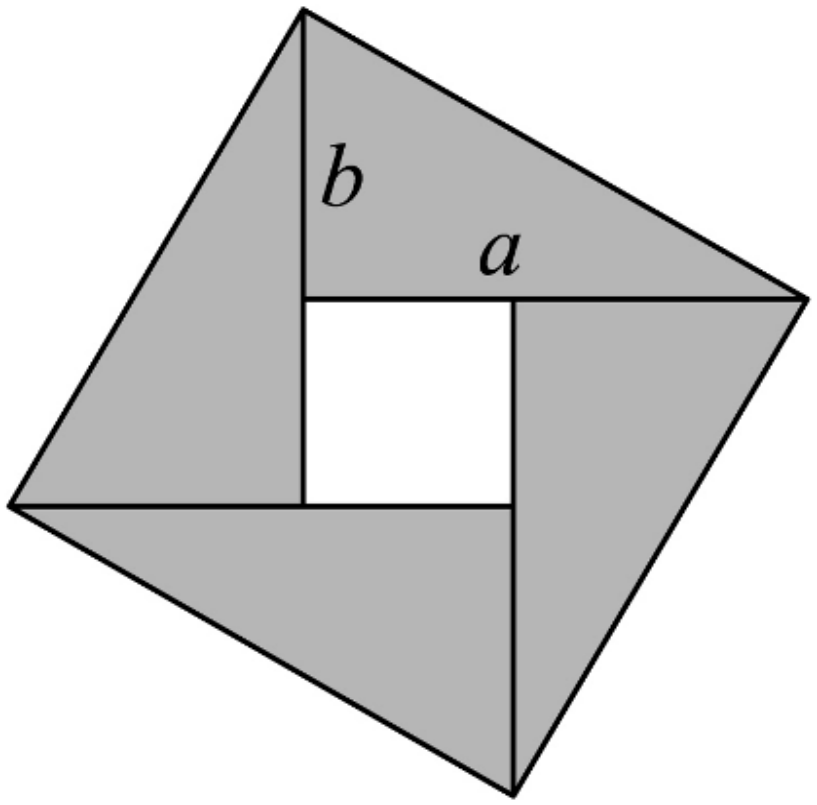
\includegraphics[width=0.20\textwidth]{figures/gao93_q16_zhaoshuang.png}
\end{center}

A. 如果 $a>b>0$，那么 $\sqrt a>\sqrt b$

B. 如果 $a>b>0$，那么 $a^2>b^2$

C. 对任意正实数 $a$ 和 $b$，有 $a^2+b^2\geqslant2ab$，当且仅当 $a=b$ 时等号成立

D. 对任意正实数 $a$ 和 $b$，有 $a^2+b^2\geqslant2ab$，当且仅当 $a=b$ 时等号成立% 原卷 C、D 两选项文字相同，照录

\ifanswer
\solbegin
\step{通过观察，可以发现这个图中的四个直角三角形是全等的，}
\step{设直角三角形的长直角边为 $a$，短直角边为 $b$，}
\step{如图，整个大正方形的面积大于等于这 $4$ 个直角三角形的面积和，}
\step{即 $a^2+b^2\geqslant4\times\left(\dfrac12ab\right)$，即 $a^2+b^2\geqslant2ab$，}
\step{当 $a=b$ 时，中间空白的正方形消失，即整个大正方形与 $4$ 个直角三角形重合；}
\step{其他选项通过该图无法证明. 故选 $C$.}
\solend
\fi

\end{enumerate}

\bigsec{三、解答题}

\begin{enumerate}
\setcounter{enumi}{16}

\item 已知 $x,y\in R$，比较 $x^2+y^2$ 与 $2(2x-y)-5$ 的大小.

\ansspace*[7]

\ifanswer
\solbegin
\step{因为 $x^2+y^2-2(2x-y)+5=(x-2)^2+(y+1)^2\geqslant0$，}
\step{所以 $x^2+y^2\geqslant2(2x-y)-5$.}
\solend
\fi

\item 设 $k\in\R$，求关于 $x$ 与 $y$ 的二元一次方程组 $\begin{cases}y=x+1\\ y=kx+3\end{cases}$ 的解集.

\ansspace*[9]

\ifanswer
\solbegin
\step{因为 $\begin{cases}y=x+1\\ y=kx+3\end{cases}$，两式相减，得到 $(k-1)x=-2$，}
\step{当 $k\neq1$ 时，$x=-\dfrac{2}{k-1}$，代入方程组中的第一式，得到 $y=\dfrac{k-3}{k-1}$，}
\step{此时，原方程组的解集为 $\left\{\left(-\dfrac{2}{k-1},\dfrac{k-3}{k-1}\right)\right\}$，}
\step{当 $k=1$ 时，方程 $(k-1)x=-2$ 无解，从而原方程组无解，其解集为空集.}
\step{综上，当 $k\neq1$ 时，解集为 $\left\{\left(-\dfrac{2}{k-1},\dfrac{k-3}{k-1}\right)\right\}$，}
\step{当 $k=1$ 时，解集为空集.}
\solend
\fi

\item 解下列不等式与方程组.

（1）解含绝对值的不等式：$\lvert x+1\rvert\geqslant3x$；

（2）求解不等式组 $\begin{cases}x^2-4x+3\geqslant0\\ \dfrac{x+3}{2x-1}\geqslant2\end{cases}$.

\ansspace*[10]

\ifanswer
\solbegin
\stepm{（1）}{当 $x\leqslant0$ 时，不等式显然成立，}
\step{当 $x>0$ 时，则 $(x+1)^2\geqslant9x^2$，得 $8x^2-2x-1\leqslant0$，}
\step{得 $(2x-1)(4x+1)\leqslant0$，解得 $-\dfrac14\leqslant x\leqslant\dfrac12$，由于 $x>0$，得 $0<x\leqslant\dfrac12$，}
\step{综上，不等式解集为 $\left\{x\left|x\leqslant\dfrac12\right.\right\}$.}
\stepm{（2）}{由 $x^2-4x+3\geqslant0$ 得 $(x-1)(x-3)\geqslant0$，所以 $x\leqslant1$ 或 $x\geqslant3$；}
\step{由 $\dfrac{x+3}{2x-1}\geqslant2$，得 $\dfrac{x+3}{2x-1}-2=\dfrac{-3x+5}{2x-1}\geqslant0$，即 $\dfrac{3x-5}{2x-1}\leqslant0$，}
\step{所以 $\begin{cases}(3x-5)(2x-1)\leqslant0\\ 2x-1\neq0\end{cases}$，解得 $\dfrac12<x\leqslant\dfrac53$，}
\step{所以不等式组的解集是 $\left\{x\left|\dfrac12<x\leqslant1\right.\right\}$.}
\solend
\fi

\item 已知关于 $x$ 的不等式 $2kx^2+kx-1<0$.

（1）若不等式的解集为 $\left(-\dfrac32,1\right)$，求实数 $k$ 的值；

（2）若不等式的解集为 $R$，求实数 $k$ 的取值范围.

\ansspace*[11]

\ifanswer
\solbegin
\stepm{（1）}{关于 $x$ 的不等式 $2kx^2+kx-1<0$ 的解集为 $\left(-\dfrac32,1\right)$，}
\step{所以 $-\dfrac32$ 和 $1$ 是方程 $2kx^2+kx-1=0$ 的两个实数根，}
\step{代入 $x=1$ 得 $2k+k-1=0$，解得 $k=\dfrac13$；}
\stepm{（2）}{若不等式 $2kx^2+kx-1<0$ 的解集为 $R$，}
\step{则 $k=0$ 时，不等式为 $-1<0$，满足题意；}
\step{$k\neq0$ 时，应满足 $\begin{cases}k<0\\ \Delta=k^2+8k<0\end{cases}$，解得 $-8<k<0$；}
\step{综上，实数 $k$ 的取值范围是 $-8<k\leqslant0$.}
\solend
\fi

\item 国家为了加强对烟酒生产的宏观管理，实行征收附加税政策，现知某种酒每瓶 $70$ 元，不征收附加税的时候，每年大约产销 $100$ 万瓶，若政府征收附加税，每销售 $100$ 元要征税 $R$ 元（叫做税率 $R\%$），则每年的销售将减少 $10R$ 万瓶.

（1）求出每年商店经营烟酒被征收的附加税税金 $S$（单位：万元）；

（2）若附加税税金 $S$ 不少于 $112$ 万元，且不大于 $168$ 万元，求 $R$ 的取值范围.

\ansspace*[12]

\ifanswer
\solbegin
\stepm{（1）}{由题意得 $S=70\times(100-10R)\times R\%(0\leqslant R\leqslant10)$（单位：万元）.}
\stepm{（2）}{由题意 $\begin{cases}70\times(100-10R)\times R\%\geqslant112\\ 70\times(100-10R)\times R\%\leqslant168\end{cases}$，解得 $2\leqslant R\leqslant4$ 或 $6\leqslant R\leqslant8$，}
\step{所以 $R$ 的取值范围是 $[2,4]\cup[6,8]$.}
\solend
\fi

\end{enumerate}

\end{document}
"
%
% 原始材料：微信公众号“魔都数学加油站”文章，连载“27学年高一93”；
% 原文标题“27学年高一93——2026-2027年上海市建平世纪高一上10月月考”；
% 原文链接：https://mp.weixin.qq.com/s/uqySZX3I8Q-QZ2J8MqmWiA。
% 正文为 7 张 PNG 页（`原图/高一93_建平世纪_10月月考/01..07.png`），均 4762×6735，按页序读取。
%
% 篇幅与题号：原卷自第 3 题起编号（第 1、2 题不在原文内）。填空题 3—12（10 题）、
% 选择题 13—16（4 题）、解答题 17—21（5 题），共 19 题。
%
% 讲评版：第 3、4 题只印【答案】（“$\{x\mid-1<x<1\}$”“$x$ 和 $y$ 不都是有理数”），本稿只给 \ans{}；
% 其余 17 题印【解析】，其中选择题答案在解析末句“故选 $D$／$D$／$C$／$C$”。
% 第 16 题题干右侧有一幅赵爽弦图（裁自第 4 页原图、去粉色水印后转灰度）。
%
% 副标题：原卷未印副标题。本稿按内容标作“集合与常用逻辑用语、不等式”。
%
% 原卷笔误/存疑（均照录未改，正文对应处另有 % 注）：
%   ① 第 3 题答案印作 $\{x\mid-1<x<1\}$（两端开），而 $\lvert x\rvert\leqslant1$ 的解集应为
%      $[-1,1]$（两端闭）；原卷照录，未改；
%   ② 第 16 题 C、D 两个选项**文字完全相同**（皆为“对任意正实数 $a$ 和 $b$，有
%      $a^2+b^2\geqslant2ab$，当且仅当 $a=b$ 时等号成立”），原卷重复排印；答案取 $C$，
%      本稿两个选项照录。
%
% 与原卷的排版差异：
%   ① 原卷每题下直接印【答案】/【解析】，本稿按全稿惯例将答案与解析置于答案版；
%   ② 原卷未印副标题，本稿补出；填空横线统一排 \blankline[4.4em]；
%   ③ 原卷数集记号排斜体 $R$，本稿按全稿惯例改用 $\R$；
%   ④ 第 17—21 题的子问用行内“（1）（2）（3）”段，解析中的子问标号用 \stepm；
%   ⑤ 解答题按惯例加 \ansspace；选择题括号排 \mbox{（\quad）}；
%   ⑥ 第 16 题的弦图原卷排在题干右侧、文字绕排，本稿改排为选项后的居中图。
%
% 行数核对：逐题数 \step/\stepm 条数，合计 71 条（Q3：0；Q4：0；Q5：2；Q6：3；Q7：2；
% Q8：2；Q9：4；Q10：1；Q11：3；Q12：9；Q13：5；Q14：3；Q15：5；Q16：6；Q17：2；
% Q18：6；Q19：8；Q20：7；Q21：3）。第 3、4 题只印答案，不计入 \step 账。
% 原卷解析的换行按语意合并，未逐行强拆。
%
\documentclass[a4paper,11pt]{article}
\usepackage{common}

\begin{document}

\examtitlest[7]{2026--2027 年建平世纪高一上 10 月月考}{集合与常用逻辑用语、不等式}

\bigsec{一、填空题}

\begin{enumerate}
\setcounter{enumi}{2}

\item 不等式 $\lvert x\rvert\leqslant1$ 的解集是\blankline[4.4em].

\ifanswer
\ans{$\{x\mid-1<x<1\}$}% 原卷答案两端开；|x|≤1 应为 [-1,1]，照录
\fi

\item “$x$ 和 $y$ 都是有理数”的否定形式是\blankline[4.4em].

\ifanswer
\ans{$x$ 和 $y$ 不都是有理数}
\fi

\item 已知等式 $2x^2+3x+5=2ax^2+a(3x+1)+c$ 恒成立，则 $a+c=\blankline[4.4em]$.

\ifanswer
\solbegin
\step{因为 $2x^2+3x+5=2ax^2+a(3x+1)+c$ 恒成立，}
\step{即 $2x^2+3x+5=2ax^2+3ax+(a+c)$ 恒成立，所以 $\begin{cases}2=2a\\ 3=3a\\ 5=a+c\end{cases}$，所以 $a+c=5$.}
\solend
\fi

\item 已知方程 $x^2+6x+m=0(m\in\R)$ 的两个根 $x_1$、$x_2$ 满足 $\lvert x_1-x_2\rvert=4$，则 $m$ 的值是\blankline[4.4em].

\ifanswer
\solbegin
\step{方程 $x^2+6x+m=0(m\in\R)$ 的两根为 $x_1$、$x_2$，所以 $x_1+x_2=-6$，$x_1x_2=m$，}
\step{又 $\lvert x_1-x_2\rvert=4$，则 $(x_1-x_2)^2=(x_1+x_2)^2-4x_1x_2=16$，}
\step{即 $(-6)^2-4m=16$，解得 $m=5$，检验得 $\Delta=6^2-4\times1\times5=16>0$，符合题意，所以 $m=5$.}
\solend
\fi

\item 已知 $\alpha:2m-6<x<m+5$，$\beta:-3<x<5$，若 $\alpha$ 是 $\beta$ 的必要条件，则实数 $m$ 的取值范围是\blankline[4.4em].

\ifanswer
\solbegin
\step{因为 $\alpha$ 是 $\beta$ 的必要条件，所以 $\begin{cases}2m-6\leqslant-3\\ m+5\geqslant5\\ 2m-6<m+5\end{cases}\Rightarrow0\leqslant m\leqslant\dfrac32$，}
\step{所以实数 $m$ 的取值范围是 $\left[0,\dfrac32\right]$.}
\solend
\fi

\item 已知 $-2\leqslant a\leqslant3$，$2\leqslant b\leqslant\dfrac72$，则 $a-2b$ 的取值范围为\blankline[4.4em].

\ifanswer
\solbegin
\step{因为 $-2\leqslant a\leqslant3$，$2\leqslant b\leqslant\dfrac72$，所以 $-7\leqslant-2b\leqslant-4$，所以 $-9\leqslant a-2b\leqslant-1$，}
\step{故 $a-2b$ 的取值范围为 $[-9,-1]$.}
\solend
\fi

\item 已知 $\lvert x+3\rvert+\lvert5-x\rvert>10$，则实数 $x$ 的取值范围为\blankline[4.4em].

\ifanswer
\solbegin
\step{当 $x<-3$ 时，则 $-x-3+5-x>10$，解得 $x<-4$，}
\step{当 $-3\leqslant x\leqslant5$ 时，则 $x+3+5-x=8<10$，原不等式不成立，}
\step{当 $x>5$ 时，则 $x+3+x-5>10$，解得 $x>6$，}
\step{综上所述，实数 $x$ 的取值范围为 $(-\infty,-4)\cup(6,+\infty)$.}
\solend
\fi

\item 已知集合 $A=\{(x,y)\mid y=x+1\}$，$B=\{(x,y)\mid y=-x+3\}$，则 $A\cap B=\blankline[4.4em]$.

\ifanswer
\solbegin
\step{联立 $\begin{cases}y=x+1\\ y=-x+3\end{cases}$，解得 $x=1$，$y=2$，故 $A\cap B=\{(1,2)\}$.}
\solend
\fi

\item 若关于 $x$ 的不等式组 $\begin{cases}\dfrac{x-1}{x-3}<0\\ x>a\end{cases}$ 的解集为空集，则实数 $a$ 的取值范围为\blankline[4.4em].

\ifanswer
\solbegin
\step{$\dfrac{x-1}{x-3}<0$ 等价于 $(x-1)(x-3)<0$，得 $1<x<3$，}
\step{因为 $\begin{cases}\dfrac{x-1}{x-3}<0\\ x>a\end{cases}$ 的解集为空集，}
\step{所以 $a\geqslant3$，故实数 $a$ 的取值范围为 $[3,+\infty)$.}
\solend
\fi

\item 已知由自然数组成的 $n-1$ 个元素的集合 $A=\{1,2,3,4,\cdots,n-1\}(n>1)$，非空集合 $B\subseteq A$，且对任意的 $a\in B$，都有 $n-a\in B$. 当 $n=9$ 时，则所有满足条件的集合 $B$ 的元素的和为\blankline[4.4em].

\ifanswer
\solbegin
\step{当 $n=9$ 时，$A=\{1,2,3,4,5,6,7,8\}$，}
\step{当 $B$ 中有两个元素时，集合 $B$ 可以为 $\{1,8\},\{2,7\},\{3,6\},\{4,5\}$，}
\step{元素总和为 $4\times9=36$；}
\step{当 $B$ 中有四个元素时，集合 $B$ 可以为 $\{1,8\},\{2,7\},\{3,6\},\{4,5\}$ 中任取两个的并集，}
\step{集合 $B$ 共有 $6$ 种情况，元素总和为 $6\times2\times9=108$；}
\step{当 $B$ 中有六个元素时，集合 $B$ 可以为 $\{1,8\},\{2,7\},\{3,6\},\{4,5\}$ 中任取三个的并集，}
\step{集合 $B$ 共有 $4$ 种情况，元素总和为 $4\times3\times9=12\times9=108$；}
\step{当 $B$ 中有八个元素时，$B=\{1,2,3,4,5,6,7,8\}$，元素之和为 $4\times9=36$，}
\step{所以所有满足条件的集合 $B$ 的元素总和为 $36+108+108+36=288$.}
\solend
\fi

\end{enumerate}

\bigsec{二、选择题}

\begin{enumerate}
\setcounter{enumi}{12}

\item 下列说法正确的是\mbox{（\quad）}

\keepwithprev
A. 若 $a>b$，则 $\dfrac1a<\dfrac1b$\qquad B. 若 $a>b,c>d$，则 $ac>bd$

C. 若 $a>b$，则 $ac^2>bc^2$\qquad D. 若 $ac^2>bc^2$，则 $a>b$

\ifanswer
\solbegin
\step{A：令 $a=2,b=-1$，此时 $\dfrac12>-1$，故 A 错误；}
\step{B：令 $a=2,b=-1,c=0,d=-2$，此时 $ac=0<bd=2$，故 B 错误；}
\step{C：由 $a>b$，当 $c=0$ 时，$ac^2=bc^2$，故 C 错误；}
\step{D：由 $ac^2>bc^2$，则 $c^2>0$，所以 $a>b$，故 D 正确.}
\step{故选 $D$.}
\solend
\fi

\item 不等式 $\dfrac{x-3}{x-1}\leqslant2$ 的解集是\mbox{（\quad）}

\keepwithprev
A. $(-\infty,1]$\qquad B. $[1,+\infty)$

C. $(-\infty,-1]\cup[1,+\infty)$\qquad D. $(-\infty,-1]\cup(1,+\infty)$

\ifanswer
\solbegin
\step{不等式 $\dfrac{x-3}{x-1}\leqslant2$ 可化为 $\dfrac{x-3}{x-1}-2\leqslant0$，即 $\dfrac{x-3-2(x-1)}{x-1}\leqslant0$，}
\step{化简得 $\dfrac{x+1}{x-1}\geqslant0$，等价于 $\begin{cases}(x+1)(x-1)\geqslant0\\ x\neq1\end{cases}$，解得 $x\leqslant-1$ 或 $x>1$，}
\step{所以不等式的解集为 $(-\infty,-1]\cup(1,+\infty)$. 故选 $D$.}
\solend
\fi

\item 已知集合 $M$ 和集合 $N$，那么 $M\cap N=N$ 的充要条件是\mbox{（\quad）}

\keepwithprev
A. $M\subseteq N$\qquad B. $N\subset M$\qquad C. $M\supseteq N$\qquad D. $M=N$

\ifanswer
\solbegin
\step{若 $M\subseteq N$，即集合 $M$ 是集合 $N$ 的子集，则 $M\cap N=M$，故 $A$ 错误；}
\step{若 $M=N$，则不能得到 $N\subset M$，故 $B$ 错误；}
\step{若 $M\cap N=N$，则 $M\supseteq N$，故 $C$ 正确；}
\step{当 $N$ 是 $M$ 真子集时，不能得到 $M=N$，故 $D$ 错误.}
\step{故选 $C$.}
\solend
\fi

\item 三国时期赵爽在《勾股方圆图注》中对勾股定理的证明可用现代数学表述为如图所示，我们教材中利用该图作为“（\quad）”的几何解释.

\begin{center}
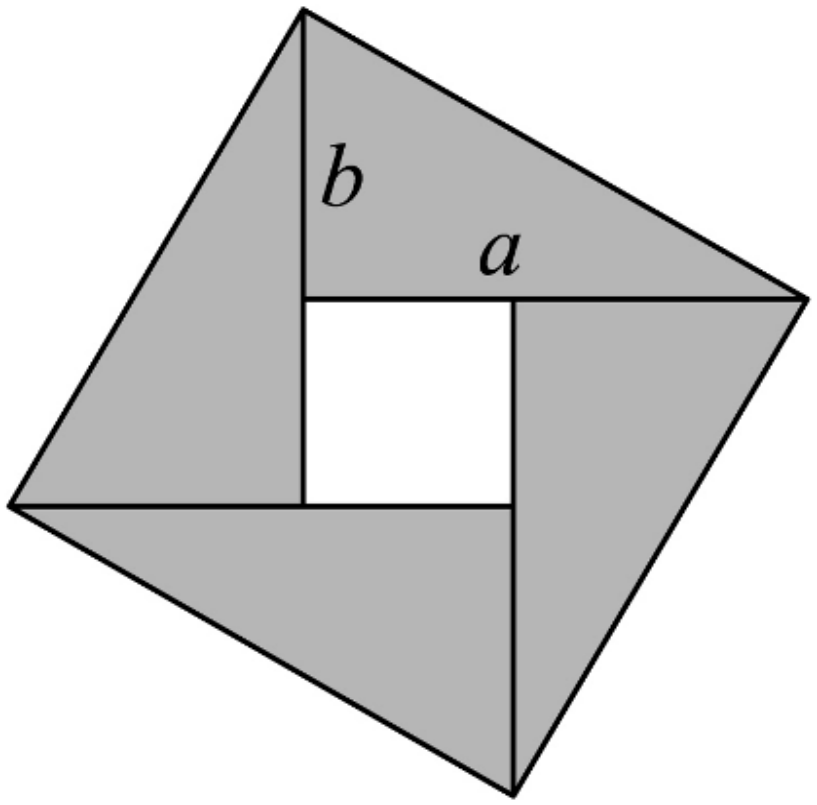
\includegraphics[width=0.20\textwidth]{figures/gao93_q16_zhaoshuang.png}
\end{center}

A. 如果 $a>b>0$，那么 $\sqrt a>\sqrt b$

B. 如果 $a>b>0$，那么 $a^2>b^2$

C. 对任意正实数 $a$ 和 $b$，有 $a^2+b^2\geqslant2ab$，当且仅当 $a=b$ 时等号成立

D. 对任意正实数 $a$ 和 $b$，有 $a^2+b^2\geqslant2ab$，当且仅当 $a=b$ 时等号成立% 原卷 C、D 两选项文字相同，照录

\ifanswer
\solbegin
\step{通过观察，可以发现这个图中的四个直角三角形是全等的，}
\step{设直角三角形的长直角边为 $a$，短直角边为 $b$，}
\step{如图，整个大正方形的面积大于等于这 $4$ 个直角三角形的面积和，}
\step{即 $a^2+b^2\geqslant4\times\left(\dfrac12ab\right)$，即 $a^2+b^2\geqslant2ab$，}
\step{当 $a=b$ 时，中间空白的正方形消失，即整个大正方形与 $4$ 个直角三角形重合；}
\step{其他选项通过该图无法证明. 故选 $C$.}
\solend
\fi

\end{enumerate}

\bigsec{三、解答题}

\begin{enumerate}
\setcounter{enumi}{16}

\item 已知 $x,y\in R$，比较 $x^2+y^2$ 与 $2(2x-y)-5$ 的大小.

\ansspace*[7]

\ifanswer
\solbegin
\step{因为 $x^2+y^2-2(2x-y)+5=(x-2)^2+(y+1)^2\geqslant0$，}
\step{所以 $x^2+y^2\geqslant2(2x-y)-5$.}
\solend
\fi

\item 设 $k\in\R$，求关于 $x$ 与 $y$ 的二元一次方程组 $\begin{cases}y=x+1\\ y=kx+3\end{cases}$ 的解集.

\ansspace*[9]

\ifanswer
\solbegin
\step{因为 $\begin{cases}y=x+1\\ y=kx+3\end{cases}$，两式相减，得到 $(k-1)x=-2$，}
\step{当 $k\neq1$ 时，$x=-\dfrac{2}{k-1}$，代入方程组中的第一式，得到 $y=\dfrac{k-3}{k-1}$，}
\step{此时，原方程组的解集为 $\left\{\left(-\dfrac{2}{k-1},\dfrac{k-3}{k-1}\right)\right\}$，}
\step{当 $k=1$ 时，方程 $(k-1)x=-2$ 无解，从而原方程组无解，其解集为空集.}
\step{综上，当 $k\neq1$ 时，解集为 $\left\{\left(-\dfrac{2}{k-1},\dfrac{k-3}{k-1}\right)\right\}$，}
\step{当 $k=1$ 时，解集为空集.}
\solend
\fi

\item 解下列不等式与方程组.

（1）解含绝对值的不等式：$\lvert x+1\rvert\geqslant3x$；

（2）求解不等式组 $\begin{cases}x^2-4x+3\geqslant0\\ \dfrac{x+3}{2x-1}\geqslant2\end{cases}$.

\ansspace*[10]

\ifanswer
\solbegin
\stepm{（1）}{当 $x\leqslant0$ 时，不等式显然成立，}
\step{当 $x>0$ 时，则 $(x+1)^2\geqslant9x^2$，得 $8x^2-2x-1\leqslant0$，}
\step{得 $(2x-1)(4x+1)\leqslant0$，解得 $-\dfrac14\leqslant x\leqslant\dfrac12$，由于 $x>0$，得 $0<x\leqslant\dfrac12$，}
\step{综上，不等式解集为 $\left\{x\left|x\leqslant\dfrac12\right.\right\}$.}
\stepm{（2）}{由 $x^2-4x+3\geqslant0$ 得 $(x-1)(x-3)\geqslant0$，所以 $x\leqslant1$ 或 $x\geqslant3$；}
\step{由 $\dfrac{x+3}{2x-1}\geqslant2$，得 $\dfrac{x+3}{2x-1}-2=\dfrac{-3x+5}{2x-1}\geqslant0$，即 $\dfrac{3x-5}{2x-1}\leqslant0$，}
\step{所以 $\begin{cases}(3x-5)(2x-1)\leqslant0\\ 2x-1\neq0\end{cases}$，解得 $\dfrac12<x\leqslant\dfrac53$，}
\step{所以不等式组的解集是 $\left\{x\left|\dfrac12<x\leqslant1\right.\right\}$.}
\solend
\fi

\item 已知关于 $x$ 的不等式 $2kx^2+kx-1<0$.

（1）若不等式的解集为 $\left(-\dfrac32,1\right)$，求实数 $k$ 的值；

（2）若不等式的解集为 $R$，求实数 $k$ 的取值范围.

\ansspace*[11]

\ifanswer
\solbegin
\stepm{（1）}{关于 $x$ 的不等式 $2kx^2+kx-1<0$ 的解集为 $\left(-\dfrac32,1\right)$，}
\step{所以 $-\dfrac32$ 和 $1$ 是方程 $2kx^2+kx-1=0$ 的两个实数根，}
\step{代入 $x=1$ 得 $2k+k-1=0$，解得 $k=\dfrac13$；}
\stepm{（2）}{若不等式 $2kx^2+kx-1<0$ 的解集为 $R$，}
\step{则 $k=0$ 时，不等式为 $-1<0$，满足题意；}
\step{$k\neq0$ 时，应满足 $\begin{cases}k<0\\ \Delta=k^2+8k<0\end{cases}$，解得 $-8<k<0$；}
\step{综上，实数 $k$ 的取值范围是 $-8<k\leqslant0$.}
\solend
\fi

\item 国家为了加强对烟酒生产的宏观管理，实行征收附加税政策，现知某种酒每瓶 $70$ 元，不征收附加税的时候，每年大约产销 $100$ 万瓶，若政府征收附加税，每销售 $100$ 元要征税 $R$ 元（叫做税率 $R\%$），则每年的销售将减少 $10R$ 万瓶.

（1）求出每年商店经营烟酒被征收的附加税税金 $S$（单位：万元）；

（2）若附加税税金 $S$ 不少于 $112$ 万元，且不大于 $168$ 万元，求 $R$ 的取值范围.

\ansspace*[12]

\ifanswer
\solbegin
\stepm{（1）}{由题意得 $S=70\times(100-10R)\times R\%(0\leqslant R\leqslant10)$（单位：万元）.}
\stepm{（2）}{由题意 $\begin{cases}70\times(100-10R)\times R\%\geqslant112\\ 70\times(100-10R)\times R\%\leqslant168\end{cases}$，解得 $2\leqslant R\leqslant4$ 或 $6\leqslant R\leqslant8$，}
\step{所以 $R$ 的取值范围是 $[2,4]\cup[6,8]$.}
\solend
\fi

\end{enumerate}

\end{document}
"
%
% 原始材料：微信公众号“魔都数学加油站”文章，连载“27学年高一93”；
% 原文标题“27学年高一93——2026-2027年上海市建平世纪高一上10月月考”；
% 原文链接：https://mp.weixin.qq.com/s/uqySZX3I8Q-QZ2J8MqmWiA。
% 正文为 7 张 PNG 页（`原图/高一93_建平世纪_10月月考/01..07.png`），均 4762×6735，按页序读取。
%
% 篇幅与题号：原卷自第 3 题起编号（第 1、2 题不在原文内）。填空题 3—12（10 题）、
% 选择题 13—16（4 题）、解答题 17—21（5 题），共 19 题。
%
% 讲评版：第 3、4 题只印【答案】（“$\{x\mid-1<x<1\}$”“$x$ 和 $y$ 不都是有理数”），本稿只给 \ans{}；
% 其余 17 题印【解析】，其中选择题答案在解析末句“故选 $D$／$D$／$C$／$C$”。
% 第 16 题题干右侧有一幅赵爽弦图（裁自第 4 页原图、去粉色水印后转灰度）。
%
% 副标题：原卷未印副标题。本稿按内容标作“集合与常用逻辑用语、不等式”。
%
% 原卷笔误/存疑（均照录未改，正文对应处另有 % 注）：
%   ① 第 3 题答案印作 $\{x\mid-1<x<1\}$（两端开），而 $\lvert x\rvert\leqslant1$ 的解集应为
%      $[-1,1]$（两端闭）；原卷照录，未改；
%   ② 第 16 题 C、D 两个选项**文字完全相同**（皆为“对任意正实数 $a$ 和 $b$，有
%      $a^2+b^2\geqslant2ab$，当且仅当 $a=b$ 时等号成立”），原卷重复排印；答案取 $C$，
%      本稿两个选项照录。
%
% 与原卷的排版差异：
%   ① 原卷每题下直接印【答案】/【解析】，本稿按全稿惯例将答案与解析置于答案版；
%   ② 原卷未印副标题，本稿补出；填空横线统一排 \blankline[4.4em]；
%   ③ 原卷数集记号排斜体 $R$，本稿按全稿惯例改用 $\R$；
%   ④ 第 17—21 题的子问用行内“（1）（2）（3）”段，解析中的子问标号用 \stepm；
%   ⑤ 解答题按惯例加 \ansspace；选择题括号排 \mbox{（\quad）}；
%   ⑥ 第 16 题的弦图原卷排在题干右侧、文字绕排，本稿改排为选项后的居中图。
%
% 行数核对：逐题数 \step/\stepm 条数，合计 71 条（Q3：0；Q4：0；Q5：2；Q6：3；Q7：2；
% Q8：2；Q9：4；Q10：1；Q11：3；Q12：9；Q13：5；Q14：3；Q15：5；Q16：6；Q17：2；
% Q18：6；Q19：8；Q20：7；Q21：3）。第 3、4 题只印答案，不计入 \step 账。
% 原卷解析的换行按语意合并，未逐行强拆。
%
\documentclass[a4paper,11pt]{article}
\usepackage{common}

\begin{document}

\examtitlest[7]{2026--2027 年建平世纪高一上 10 月月考}{集合与常用逻辑用语、不等式}

\bigsec{一、填空题}

\begin{enumerate}
\setcounter{enumi}{2}

\item 不等式 $\lvert x\rvert\leqslant1$ 的解集是\blankline[4.4em].

\ifanswer
\ans{$\{x\mid-1<x<1\}$}% 原卷答案两端开；|x|≤1 应为 [-1,1]，照录
\fi

\item “$x$ 和 $y$ 都是有理数”的否定形式是\blankline[4.4em].

\ifanswer
\ans{$x$ 和 $y$ 不都是有理数}
\fi

\item 已知等式 $2x^2+3x+5=2ax^2+a(3x+1)+c$ 恒成立，则 $a+c=\blankline[4.4em]$.

\ifanswer
\solbegin
\step{因为 $2x^2+3x+5=2ax^2+a(3x+1)+c$ 恒成立，}
\step{即 $2x^2+3x+5=2ax^2+3ax+(a+c)$ 恒成立，所以 $\begin{cases}2=2a\\ 3=3a\\ 5=a+c\end{cases}$，所以 $a+c=5$.}
\solend
\fi

\item 已知方程 $x^2+6x+m=0(m\in\R)$ 的两个根 $x_1$、$x_2$ 满足 $\lvert x_1-x_2\rvert=4$，则 $m$ 的值是\blankline[4.4em].

\ifanswer
\solbegin
\step{方程 $x^2+6x+m=0(m\in\R)$ 的两根为 $x_1$、$x_2$，所以 $x_1+x_2=-6$，$x_1x_2=m$，}
\step{又 $\lvert x_1-x_2\rvert=4$，则 $(x_1-x_2)^2=(x_1+x_2)^2-4x_1x_2=16$，}
\step{即 $(-6)^2-4m=16$，解得 $m=5$，检验得 $\Delta=6^2-4\times1\times5=16>0$，符合题意，所以 $m=5$.}
\solend
\fi

\item 已知 $\alpha:2m-6<x<m+5$，$\beta:-3<x<5$，若 $\alpha$ 是 $\beta$ 的必要条件，则实数 $m$ 的取值范围是\blankline[4.4em].

\ifanswer
\solbegin
\step{因为 $\alpha$ 是 $\beta$ 的必要条件，所以 $\begin{cases}2m-6\leqslant-3\\ m+5\geqslant5\\ 2m-6<m+5\end{cases}\Rightarrow0\leqslant m\leqslant\dfrac32$，}
\step{所以实数 $m$ 的取值范围是 $\left[0,\dfrac32\right]$.}
\solend
\fi

\item 已知 $-2\leqslant a\leqslant3$，$2\leqslant b\leqslant\dfrac72$，则 $a-2b$ 的取值范围为\blankline[4.4em].

\ifanswer
\solbegin
\step{因为 $-2\leqslant a\leqslant3$，$2\leqslant b\leqslant\dfrac72$，所以 $-7\leqslant-2b\leqslant-4$，所以 $-9\leqslant a-2b\leqslant-1$，}
\step{故 $a-2b$ 的取值范围为 $[-9,-1]$.}
\solend
\fi

\item 已知 $\lvert x+3\rvert+\lvert5-x\rvert>10$，则实数 $x$ 的取值范围为\blankline[4.4em].

\ifanswer
\solbegin
\step{当 $x<-3$ 时，则 $-x-3+5-x>10$，解得 $x<-4$，}
\step{当 $-3\leqslant x\leqslant5$ 时，则 $x+3+5-x=8<10$，原不等式不成立，}
\step{当 $x>5$ 时，则 $x+3+x-5>10$，解得 $x>6$，}
\step{综上所述，实数 $x$ 的取值范围为 $(-\infty,-4)\cup(6,+\infty)$.}
\solend
\fi

\item 已知集合 $A=\{(x,y)\mid y=x+1\}$，$B=\{(x,y)\mid y=-x+3\}$，则 $A\cap B=\blankline[4.4em]$.

\ifanswer
\solbegin
\step{联立 $\begin{cases}y=x+1\\ y=-x+3\end{cases}$，解得 $x=1$，$y=2$，故 $A\cap B=\{(1,2)\}$.}
\solend
\fi

\item 若关于 $x$ 的不等式组 $\begin{cases}\dfrac{x-1}{x-3}<0\\ x>a\end{cases}$ 的解集为空集，则实数 $a$ 的取值范围为\blankline[4.4em].

\ifanswer
\solbegin
\step{$\dfrac{x-1}{x-3}<0$ 等价于 $(x-1)(x-3)<0$，得 $1<x<3$，}
\step{因为 $\begin{cases}\dfrac{x-1}{x-3}<0\\ x>a\end{cases}$ 的解集为空集，}
\step{所以 $a\geqslant3$，故实数 $a$ 的取值范围为 $[3,+\infty)$.}
\solend
\fi

\item 已知由自然数组成的 $n-1$ 个元素的集合 $A=\{1,2,3,4,\cdots,n-1\}(n>1)$，非空集合 $B\subseteq A$，且对任意的 $a\in B$，都有 $n-a\in B$. 当 $n=9$ 时，则所有满足条件的集合 $B$ 的元素的和为\blankline[4.4em].

\ifanswer
\solbegin
\step{当 $n=9$ 时，$A=\{1,2,3,4,5,6,7,8\}$，}
\step{当 $B$ 中有两个元素时，集合 $B$ 可以为 $\{1,8\},\{2,7\},\{3,6\},\{4,5\}$，}
\step{元素总和为 $4\times9=36$；}
\step{当 $B$ 中有四个元素时，集合 $B$ 可以为 $\{1,8\},\{2,7\},\{3,6\},\{4,5\}$ 中任取两个的并集，}
\step{集合 $B$ 共有 $6$ 种情况，元素总和为 $6\times2\times9=108$；}
\step{当 $B$ 中有六个元素时，集合 $B$ 可以为 $\{1,8\},\{2,7\},\{3,6\},\{4,5\}$ 中任取三个的并集，}
\step{集合 $B$ 共有 $4$ 种情况，元素总和为 $4\times3\times9=12\times9=108$；}
\step{当 $B$ 中有八个元素时，$B=\{1,2,3,4,5,6,7,8\}$，元素之和为 $4\times9=36$，}
\step{所以所有满足条件的集合 $B$ 的元素总和为 $36+108+108+36=288$.}
\solend
\fi

\end{enumerate}

\bigsec{二、选择题}

\begin{enumerate}
\setcounter{enumi}{12}

\item 下列说法正确的是\mbox{（\quad）}

\keepwithprev
A. 若 $a>b$，则 $\dfrac1a<\dfrac1b$\qquad B. 若 $a>b,c>d$，则 $ac>bd$

C. 若 $a>b$，则 $ac^2>bc^2$\qquad D. 若 $ac^2>bc^2$，则 $a>b$

\ifanswer
\solbegin
\step{A：令 $a=2,b=-1$，此时 $\dfrac12>-1$，故 A 错误；}
\step{B：令 $a=2,b=-1,c=0,d=-2$，此时 $ac=0<bd=2$，故 B 错误；}
\step{C：由 $a>b$，当 $c=0$ 时，$ac^2=bc^2$，故 C 错误；}
\step{D：由 $ac^2>bc^2$，则 $c^2>0$，所以 $a>b$，故 D 正确.}
\step{故选 $D$.}
\solend
\fi

\item 不等式 $\dfrac{x-3}{x-1}\leqslant2$ 的解集是\mbox{（\quad）}

\keepwithprev
A. $(-\infty,1]$\qquad B. $[1,+\infty)$

C. $(-\infty,-1]\cup[1,+\infty)$\qquad D. $(-\infty,-1]\cup(1,+\infty)$

\ifanswer
\solbegin
\step{不等式 $\dfrac{x-3}{x-1}\leqslant2$ 可化为 $\dfrac{x-3}{x-1}-2\leqslant0$，即 $\dfrac{x-3-2(x-1)}{x-1}\leqslant0$，}
\step{化简得 $\dfrac{x+1}{x-1}\geqslant0$，等价于 $\begin{cases}(x+1)(x-1)\geqslant0\\ x\neq1\end{cases}$，解得 $x\leqslant-1$ 或 $x>1$，}
\step{所以不等式的解集为 $(-\infty,-1]\cup(1,+\infty)$. 故选 $D$.}
\solend
\fi

\item 已知集合 $M$ 和集合 $N$，那么 $M\cap N=N$ 的充要条件是\mbox{（\quad）}

\keepwithprev
A. $M\subseteq N$\qquad B. $N\subset M$\qquad C. $M\supseteq N$\qquad D. $M=N$

\ifanswer
\solbegin
\step{若 $M\subseteq N$，即集合 $M$ 是集合 $N$ 的子集，则 $M\cap N=M$，故 $A$ 错误；}
\step{若 $M=N$，则不能得到 $N\subset M$，故 $B$ 错误；}
\step{若 $M\cap N=N$，则 $M\supseteq N$，故 $C$ 正确；}
\step{当 $N$ 是 $M$ 真子集时，不能得到 $M=N$，故 $D$ 错误.}
\step{故选 $C$.}
\solend
\fi

\item 三国时期赵爽在《勾股方圆图注》中对勾股定理的证明可用现代数学表述为如图所示，我们教材中利用该图作为“（\quad）”的几何解释.

\begin{center}
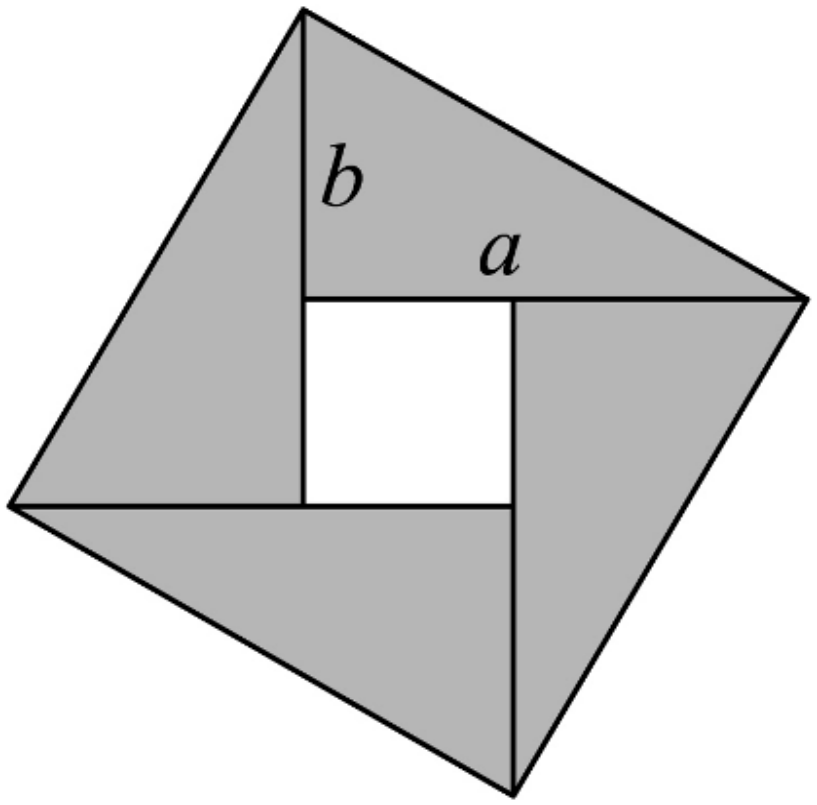
\includegraphics[width=0.20\textwidth]{figures/gao93_q16_zhaoshuang.png}
\end{center}

A. 如果 $a>b>0$，那么 $\sqrt a>\sqrt b$

B. 如果 $a>b>0$，那么 $a^2>b^2$

C. 对任意正实数 $a$ 和 $b$，有 $a^2+b^2\geqslant2ab$，当且仅当 $a=b$ 时等号成立

D. 对任意正实数 $a$ 和 $b$，有 $a^2+b^2\geqslant2ab$，当且仅当 $a=b$ 时等号成立% 原卷 C、D 两选项文字相同，照录

\ifanswer
\solbegin
\step{通过观察，可以发现这个图中的四个直角三角形是全等的，}
\step{设直角三角形的长直角边为 $a$，短直角边为 $b$，}
\step{如图，整个大正方形的面积大于等于这 $4$ 个直角三角形的面积和，}
\step{即 $a^2+b^2\geqslant4\times\left(\dfrac12ab\right)$，即 $a^2+b^2\geqslant2ab$，}
\step{当 $a=b$ 时，中间空白的正方形消失，即整个大正方形与 $4$ 个直角三角形重合；}
\step{其他选项通过该图无法证明. 故选 $C$.}
\solend
\fi

\end{enumerate}

\bigsec{三、解答题}

\begin{enumerate}
\setcounter{enumi}{16}

\item 已知 $x,y\in R$，比较 $x^2+y^2$ 与 $2(2x-y)-5$ 的大小.

\ansspace*[7]

\ifanswer
\solbegin
\step{因为 $x^2+y^2-2(2x-y)+5=(x-2)^2+(y+1)^2\geqslant0$，}
\step{所以 $x^2+y^2\geqslant2(2x-y)-5$.}
\solend
\fi

\item 设 $k\in\R$，求关于 $x$ 与 $y$ 的二元一次方程组 $\begin{cases}y=x+1\\ y=kx+3\end{cases}$ 的解集.

\ansspace*[9]

\ifanswer
\solbegin
\step{因为 $\begin{cases}y=x+1\\ y=kx+3\end{cases}$，两式相减，得到 $(k-1)x=-2$，}
\step{当 $k\neq1$ 时，$x=-\dfrac{2}{k-1}$，代入方程组中的第一式，得到 $y=\dfrac{k-3}{k-1}$，}
\step{此时，原方程组的解集为 $\left\{\left(-\dfrac{2}{k-1},\dfrac{k-3}{k-1}\right)\right\}$，}
\step{当 $k=1$ 时，方程 $(k-1)x=-2$ 无解，从而原方程组无解，其解集为空集.}
\step{综上，当 $k\neq1$ 时，解集为 $\left\{\left(-\dfrac{2}{k-1},\dfrac{k-3}{k-1}\right)\right\}$，}
\step{当 $k=1$ 时，解集为空集.}
\solend
\fi

\item 解下列不等式与方程组.

（1）解含绝对值的不等式：$\lvert x+1\rvert\geqslant3x$；

（2）求解不等式组 $\begin{cases}x^2-4x+3\geqslant0\\ \dfrac{x+3}{2x-1}\geqslant2\end{cases}$.

\ansspace*[10]

\ifanswer
\solbegin
\stepm{（1）}{当 $x\leqslant0$ 时，不等式显然成立，}
\step{当 $x>0$ 时，则 $(x+1)^2\geqslant9x^2$，得 $8x^2-2x-1\leqslant0$，}
\step{得 $(2x-1)(4x+1)\leqslant0$，解得 $-\dfrac14\leqslant x\leqslant\dfrac12$，由于 $x>0$，得 $0<x\leqslant\dfrac12$，}
\step{综上，不等式解集为 $\left\{x\left|x\leqslant\dfrac12\right.\right\}$.}
\stepm{（2）}{由 $x^2-4x+3\geqslant0$ 得 $(x-1)(x-3)\geqslant0$，所以 $x\leqslant1$ 或 $x\geqslant3$；}
\step{由 $\dfrac{x+3}{2x-1}\geqslant2$，得 $\dfrac{x+3}{2x-1}-2=\dfrac{-3x+5}{2x-1}\geqslant0$，即 $\dfrac{3x-5}{2x-1}\leqslant0$，}
\step{所以 $\begin{cases}(3x-5)(2x-1)\leqslant0\\ 2x-1\neq0\end{cases}$，解得 $\dfrac12<x\leqslant\dfrac53$，}
\step{所以不等式组的解集是 $\left\{x\left|\dfrac12<x\leqslant1\right.\right\}$.}
\solend
\fi

\item 已知关于 $x$ 的不等式 $2kx^2+kx-1<0$.

（1）若不等式的解集为 $\left(-\dfrac32,1\right)$，求实数 $k$ 的值；

（2）若不等式的解集为 $R$，求实数 $k$ 的取值范围.

\ansspace*[11]

\ifanswer
\solbegin
\stepm{（1）}{关于 $x$ 的不等式 $2kx^2+kx-1<0$ 的解集为 $\left(-\dfrac32,1\right)$，}
\step{所以 $-\dfrac32$ 和 $1$ 是方程 $2kx^2+kx-1=0$ 的两个实数根，}
\step{代入 $x=1$ 得 $2k+k-1=0$，解得 $k=\dfrac13$；}
\stepm{（2）}{若不等式 $2kx^2+kx-1<0$ 的解集为 $R$，}
\step{则 $k=0$ 时，不等式为 $-1<0$，满足题意；}
\step{$k\neq0$ 时，应满足 $\begin{cases}k<0\\ \Delta=k^2+8k<0\end{cases}$，解得 $-8<k<0$；}
\step{综上，实数 $k$ 的取值范围是 $-8<k\leqslant0$.}
\solend
\fi

\item 国家为了加强对烟酒生产的宏观管理，实行征收附加税政策，现知某种酒每瓶 $70$ 元，不征收附加税的时候，每年大约产销 $100$ 万瓶，若政府征收附加税，每销售 $100$ 元要征税 $R$ 元（叫做税率 $R\%$），则每年的销售将减少 $10R$ 万瓶.

（1）求出每年商店经营烟酒被征收的附加税税金 $S$（单位：万元）；

（2）若附加税税金 $S$ 不少于 $112$ 万元，且不大于 $168$ 万元，求 $R$ 的取值范围.

\ansspace*[12]

\ifanswer
\solbegin
\stepm{（1）}{由题意得 $S=70\times(100-10R)\times R\%(0\leqslant R\leqslant10)$（单位：万元）.}
\stepm{（2）}{由题意 $\begin{cases}70\times(100-10R)\times R\%\geqslant112\\ 70\times(100-10R)\times R\%\leqslant168\end{cases}$，解得 $2\leqslant R\leqslant4$ 或 $6\leqslant R\leqslant8$，}
\step{所以 $R$ 的取值范围是 $[2,4]\cup[6,8]$.}
\solend
\fi

\end{enumerate}

\end{document}
